%% Le lingue utilizzate, che verranno passate come opzioni al pacchetto babel. Come sempre, l'ultima indicata sar� quella primaria.
%% Se si utilizzano una o pi� lingue diverse da "italian" o "english", leggere le istruzioni in fondo.
\def\thudbabelopt{english,italian}
%% Valori ammessi per target: bach (tesi triennale), mst (tesi magistrale), phd (tesi di dottorato).
\documentclass[target=bach, hidelinks]{thud}[2019/02/22]

%% --- Informazioni sulla tesi ---
%% Per tutti i tipi di tesi
\title{Analisi e implementazione di Euristiche per il Traveling Salesman Problem}
\author{Brian Riccardi}
\course{Informatica}
\supervisor{Prof.\ Giuseppe Lancia}
% \date{2018-2019}
%% Altri campi disponibili: \reviewer, \tutor, \chair, \date (anno accademico, calcolato in automatico).
%% Con \supervisor, \cosupervisor, \reviewer e \tutor si possono indicare pi� nomi separati da \and.

%% --- Pacchetti consigliati ---
%% hyperref: Regola le impostazioni della creazione del PDF... pi� tante altre cose.
%% tocbibind: Inserisce nell'indice anche la lista delle figure, la bibliografia, ecc.

%% --- Stili di pagina disponibili (comando \pagestyle) ---
%% sfbig (predefinito): Apertura delle parti e dei capitoli col numero grande; titoli delle parti e dei capitoli e intestazioni di pagina in sans serif.
%% big: Come "sfbig", solo serif.
%% plain: Apertura delle parti e dei capitoli tradizionali di LaTeX; intestazioni di pagina come "big".

\raggedbottom
\usepackage{amssymb, amsmath, amsthm, mathrsfs}
\usepackage{algorithm}
\usepackage{algpseudocode}
\usepackage{subcaption}
\usepackage{float}
\usepackage[a-1b]{pdfx}
\usepackage[pdfa]{hyperref}

\newtheorem{definition}{Definizione}[section]
\newtheorem*{definition*}{Definizioni}
\newtheorem{observation}{Osservazione}[section]
\newtheorem{theorem}{Teorema}[section]
\newtheorem{case}{Caso}
% \newtheorem{proof}{Dimostrazione}[chapter]
\newcommand{\opt}[3]{\xrightarrow[#3]{#1,#2}}
\newcommand*{\pls}{\oplus}
\newcommand*{\mns}{\ominus}
\newcommand*{\taup}[2]{\tau^+\!(#1,#2)}
\newcommand*{\taum}[2]{\tau^-\!(#1,#2)}
\newcommand*{\norm}[1]{\lVert#1\rVert}
\algnewcommand\algorithmicforeach{\textbf{for each}}
\algdef{S}[FOR]{ForEach}[1]{\algorithmicforeach\ #1\ \algorithmicdo}



\begin{document}

%% Il frontespizio prima di tutto!
\maketitle

%% Dedica (opzionale)
% \begin{dedication}Al mio cane,\par per avermi ascoltato mentre ripassavo le lezioni.\end{dedication}

%% Ringraziamenti (opzionali)
% \acknowledgements
% Sed vel lorem a arcu faucibus aliquet eu semper tortor. Aliquam dolor lacus, semper vitae ligula sed, blandit iaculis leo. Nam pharetra lobortis leo nec auctor. Pellentesque habitant morbi tristique senectus et netus et malesuada fames ac turpis egestas. Fusce ac risus pulvinar, congue eros non, interdum metus. Mauris tincidunt neque et aliquam imperdiet. Aenean ac tellus id nibh pellentesque pulvinar ut eu lacus. Proin tempor facilisis tortor, et hendrerit purus commodo laoreet. Quisque sed augue id ligula consectetur adipiscing. Vestibulum libero metus, lacinia ac vestibulum eu, varius non arcu. Nam et gravida velit.

%% Sommario (opzionale)
% \abstract
% Nunc ac dignissim ipsum, quis pulvinar elit. Mauris congue nec leo ornare lobortis. Nulla hendrerit pretium diam nec lobortis. Nullam aliquam laoreet nisl, sit amet facilisis lectus accumsan ut. Duis et elit hendrerit metus venenatis condimentum. Integer id eros molestie, interdum leo sit amet, aliquet metus. Integer fermentum tristique magna, vel luctus neque rhoncus vel. Ut hendrerit et quam et semper. Mauris egestas, odio sed aliquet luctus, magna orci euismod odio, vitae lacinia tellus tellus non lectus. Aliquam urna neque, porta et mattis aliquam, congue sit amet lorem. In ultrices augue sit amet ante vehicula, vitae rhoncus turpis auctor. Donec porta scelerisque eros, at mollis enim imperdiet ut. 

%% Indice
\tableofcontents

%% Lista delle tabelle (se presenti)
%\listoftables

%% Lista delle figure (se presenti)
% \listoffigures

%% Corpo principale del documento
\mainmatter

% Introduzione
\chapter*{Introduzione}

Il Problema del Commesso Viaggiatore consiste nella ricerca del Circuito Hamiltoniano
di costo minimo in un grafo pesato. Formalmente, dato un grafo $G=(V,E)$ e una funzione di peso
$w: E \rightarrow \mathbb{N}$ siamo interessati ad una permutazione dei vertici del grafo
$(v_{i_1}, v_{i_2}, \dots, v_{i_{|V|}})$ che minimizzi la quantità
$$W = w(v_{i_{|V|}}, v_{i_1}) \;+ \displaystyle\sum_{j=1}^{|V|-1}{w(v_{i_j}, v_{i_{j+1}})}$$

Nell'ambito della Ricerca Operativa e dell'Ottimizzazione
Combinatoria, l'importanza del TSP (dall'inglese \textit{Traveling Salesman Problem}) deriva dal 
fatto di poterlo utilizzare per descrivere un ricco insieme di \textit{real world problems} riguardo, 
ad esempio, Cristallografia, \textit{Vehicle routing}, \textit{Scheduling}, Robotica, ecc...

Dal punto di vista teorico, la versione decisionale di TSP è notoriamente NP-Completa e ciò lo
rende, nella pratica, intrattabile anche per piccole istanze del problema.
Dalla necessità di risolvere il TSP e dall'impossibilità (assumendo $P\neq{}NP$) di poterlo
fare efficientemente per una qualsiasi istanza del problema, nasce il concetto di ``Euristica'', ovvero una tecnica che ha
lo scopo di trovare in un tempo ragionevole un'approssimazione sufficientemente buona della soluzione esatta.
\ \\
Nell'ambito del TSP possiamo dividere le euristiche in tre classi:
\begin{itemize}
    \item Tour construction: l'algoritmo costruisce il circuito aggiungendo, passo dopo passo, un nuovo
            vertice a seconda di una strategia più o meno elaborata
    %
    \item Tour improvement: a partire da un circuito arbitrario, l'algoritmo esegue delle ``mosse'' che hanno
            lo scopo di migliorarlo
    %
    \item Composite: vengono combinate le tecniche di costruzione e di miglioramento
\end{itemize}

In questa tesi studieremo il Commesso Viaggiatore Simmetrico (STSP), ovvero assumeremo
che il grafo sia non diretto, completo e con funzione di peso simmetrica. Presenteremo delle euristiche
appartenenti ad ognuna delle classi e ne analizzeremo le performance sia dal punto di vista dell'efficienza
in tempo, sia dal punto di vista dell'efficacia nel senso della bontà della soluzione trovata rispetto all'ottimo.
Gli algoritmi scelti sono Nearest Neighbor, Nearest Insertion, Christofides, 3-OPT (in tre versioni) e 
Lin-Kernighan-Helsgaun: per quanto riguarda Christofides e Lin-Kernighan-Helsgaun si è deciso di implementare 
una versione più semplice degli algoritmi in letteratura; possiamo quindi dire che le euristiche implementate 
siano solamente ispirate a quelle descritte in \cite{CHR}, \cite{LKH}; per quanto riguarda 3-OPT, 
si è scelto di implementare la versione descritta in \cite{3opt}.

I test sono stati effettuati su un insieme di grafi selezionati da TSPLIB\cite{tsplib} e su un insieme di grafi generati
casualmente. Le misurazioni sono state effettuate seguendo le procedure descritte in \cite{Poli}. Tutti i programmi sono 
stati scritti in \texttt{C++}.


% % STSP teoria e pratica
\chapter{Il Commesso Viaggiatore}

Il Problema del Commesso Viaggiatore può essere formulato, informalmente, in questo modo:\\
\ \\
``Un commerciante deve visitare $n$ città in modo tale da visitarle tutte una e una sola volta, 
ritornando al punto di partenza. Ogni coppia di città $(i,j)$ è collegata da una strada e ogni strada, 
per essere percorsa, necessita il pagamento di un pedaggio. Il commerciante, essendo molto avido, vuole 
trovare il percorso che gli assicuri di spendere il meno possibile.''
\ \\
\ \\
Nonostante la facilità con cui venga espresso, il Commesso Viaggiatore è tutt'altro che semplice
da risolvere. È un problema di Ottimizzazione Combinatoria noto da decenni e, date le sue potenzialmente 
infinite applicazioni pratiche, è ancora oggi uno dei problemi più studiati. Dal punto di vista formale, 
il TSP (dall'inglese \textit{Traveling Salesman Problem}) consiste nella ricerca del Circuito Hamiltoniano di 
costo minimo in un grafo pesato. È possibile dare diverse formulazioni equivalenti al problema: di seguito
ne diamo due.

\begin{definition}[\textbf{TSP su grafi}]
    Sia $G=(V,E)$ un grafo di $n$ vertici completo e pesato con funzione di peso $w:E \rightarrow \mathbb{N}$.
    Vogliamo determinare una permutazione dei vertici $(v_1,v_2,\dots,v_n)$ tale che
    $$w(v_n,v_1) + \displaystyle\sum_{i=1}^{n-1}{w(v_i,v_{i+1})}$$
    sia minima.
\end{definition}

\begin{definition}[\textbf{TSP su matrici}]
    Sia $n \in \mathbb{N}_+$ e $C=(c_{i,j})$ una matrice $n\times{}n$ a valori in $\mathbb{N}$ tale che 
    $c_{i,i}=0$ per ogni $i\in\{1,2,\dots,n\}$. Determinare una permutazione $(i_1,i_2,\dots,i_n)$
    di $(1,2,\dots,n)$ tale che
    $$c_{i_n,i_1} + \displaystyle\sum_{j=1}^{n-1}{c_{i_j,i_{j+1}}}$$
    sia minima.
\end{definition}

Le due definizioni sono banalmente equivalenti e ne verrà utilizzata una piuttosto che l'altra in base 
al contesto. Inoltre, diamo alcune definizioni ``classiche'' e convenzioni.

\begin{definition*}\ \\
    (1) Un tour è una permutazione dei vertici.\\
    (2) Costo e peso verranno utilizzati come sinonimi.\\
    (3) Il Commesso Viaggiatore Simmetrico (STSP) consiste nell'ulteriore ipotesi che la matrice $C$ sia simmetrica.\\
    (4) Per istanza geometrica si intende che $w$ soddisfa la disuguaglianza triangolare.\\
    (5) Per istanza euclidea si intende che $w$ è la funzione di distanza euclidea.
\end{definition*}
\ \\

La relazione che TSP sembra avere con il problema del Circuito Hamiltoniano (HAM-CYCLE) sottintende una 
difficoltà computazionale quantomeno simile. Definiamo innanzitutto il linguaggio che stiamo considerando.
\begin{definition}[\textbf{TSP} come linguaggio formale]
    \begin{align*}
    \textbf{TSP} =\{\langle G,w,k\rangle \;:\; & G = (V,E) \text{ è un grafo completo},\\
                                            & w: E \rightarrow \mathbb{R} \text{ è una funzione di costo},\\
                                            & k \in \mathbb{N},\\
                                            & G \text{ possiede un tour hamiltoniano di costo } \leq k\}
    \end{align*}
\end{definition}

\begin{theorem}
    \textbf{TSP} è NP-Completo.
\end{theorem}

\begin{proof}
    La dimostrazione viene fatta separando l'appartenenza ad NP dalla hardness.
    \begin{description}
        \item[\textbf{TSP $\in$ NP:}] consideriamo un'istanza di \textbf{TSP} e una soluzione.
                La verifica della soluzione può essere svolta in tempo polinomiale: si controlla che ogni 
                vertice appartenga alla soluzione e si controlla che la somma dei pesi degli archi sia al più $k$.
                Per \textit{Guess\&Verify} \textbf{TSP} è in NP.

        \item[\textbf{TSP $\in$ NP-hard:}] mostriamo che \textbf{HAM-CYCLE} $\preceq$ \textbf{TSP}.\\
                Sia $G=(V,E)$ un'instanza di \textbf{HAM-CYCLE}. Costruiamo $G'$, completo e pesato con funzione 
                $$w(i,j) = \begin{cases}
                            0 & \text{se } (i,j) \in E\\
                            1 & \text{se } (i,j) \notin E
                            \end{cases}$$
                Consideriamo quindi l'istanza $\langle G',w,0\rangle $ di \textbf{ TSP}. Si ha quindi che 
                se $\langle G\rangle \in \textbf{HAM-CYCLE}$ allora esiste un circuito hamiltoniano in G, ma 
                per costruzione $G'$ ammette un circuito hamiltoniano di costo $0$, quindi 
                $\langle G',w,0\rangle \in \textbf{TSP}$.\\
                Al contrario, se $\langle G',w,0\rangle \in \textbf{TSP}$ allora $G'$ ammette un circuito 
                hamiltoniano di costo $0$ e, per $w$, ogni arco del circuito ha costo $0$. Ma allora ogni 
                arco del circuito è in $E$ e quindi anche $G$ ammette un circuito hamiltoniano, quindi 
                $\langle G\rangle \in \textbf{HAM-CYCLE}$.
    \end{description}
\end{proof}

% % Euristiche
\chapter{Euristiche per il TSP}

Dalla \textit{Hardness} di TSP si evince che una sua risoluzione esatta, per ogni istanza del problema,
sia computazionalmente intrattabile anche per grafi di modeste dimensioni. L'importanza dei risvolti 
applicativi, tuttavia, ci costringe a non abbandonare completamente il suo studio e anzi ci spinge
ad indagare più a fondo alla ricerca di tecniche per aggirare il vincolo computazionale. Vi sono infatti
almeno tre strade che possiamo percorrere: se l'istanza è piccola allora un approccio \textit{bruteforce}
è ancora utilizzabile; è possibile tentare di risolvere casi particolari, (\textit{e.g.} un'istanza 
euclidea che ammette una \textit{collana}\cite{Neck}); è possibile accettare soluzioni \textit{quasi-ottime}. 
Quest'ultimo è l'approccio di tipo euristico e, generalmente, soluzioni vicine all'ottimalità sono più che sufficienti. 
Occorre quindi definire chiaramente quello che intendiamo quando parliamo di soluzioni ``quasi-ottime''.

\begin{definition}[\textbf{$\rho{}$-approssimazione}]
    Sia $\mathcal{P}$ un problema di minimizzazione, $\mathcal{A}$ un'euristica per
    $\mathcal{P}$ e $\rho{}:\mathbb{N}\rightarrow{}\mathbb{R}$. Diremo che
    $\mathcal{A}$ è $\rho$-approssimato se per ogni istanza $x \in \mathcal{P}$ di dimensione $n$ con soluzione
    esatta \textbf{OPT} si ha $\mathcal{A}(n) \leq \rho{}(n)\textbf{OPT}$. Diremo inoltre che $\rho$
    è il rapporto di approssimazione di $\mathcal{A}$.

\end{definition}
\ \\
\ \\
Nel caso del TSP possiamo suddividere le euristiche in tre categorie.

\section{Tour construction}

Nelle euristiche di tipo ``tour construction'' il circuito viene costruito incrementalmente e l'algoritmo
termina appena il tour così creato è valido. Di seguito elenchiamo diversi esempi di euristiche basate
sul tour construction.
\ \\

\subsection{Strip (\texttt{STRIP})}

Questa euristica viene applicata su istanze \textit{geometriche} di STSP. L'idea è quella
di cercare il minimo rettangolo che contiene tutti i punti del problema, suddividerlo in $\sqrt{\frac{N}{3}}$
\textit{strips} verticali e costruire il tour immaginando di percorrere ogni strip verticalmente, alternando il
verso di percorrenza ad ogni nuova strip. Il tour verrà quindi chiuso collegando l'ultimo punto con il primo.
La ricerca del rettangolo minimo può essere svolta linearmente scandendo l'insieme dei punti e memorizzandone
le coordinate estremali (min/max ascissa e min/max ordinata). La suddivisione dei punti nelle strisce può
essere ancora svolta linearmente. La scansione ordinata dei punti nella strip può essere simulata
ordinando preventivamente i punti per ordinata scegliendo un sorting in senso crescente o decrescente
a secondo di quale strip si consideri. I vantaggi principali di questa euristica sono senza dubbio la semplicità
concettuale e implementativa, nonché la velocità di esecuzione. Tuttavia, è facile notare come \texttt{STRIP}
abbia un rapporto di approssimazione $\rho(n) \in \Omega(\sqrt{n})$: si pensi infatti ad un'instanza in cui i punti
siano ai limiti delle strip. Per punti uniformemente distribuiti nel quadrato unitario, il
tour prodotto è in media non più lungo di $0.93\sqrt{n}$\cite{STRIP}.
\ \\

\subsection{Nearest Neighbor (\texttt{NN})}

L'idea è quella di avere, ad ogni passo, un tour parziale da estendere
aggiungendo un vertice non ancora presente che sia a distanza minima dal vertice aggiunto al passo precedente.

\begin{algorithm}[H]
\caption{}
\begin{algorithmic}[1]
\Function{NearestNeighbor}{$G=(V,E), w$}
    \State $n \gets |V|$
    \State $v \gets \texttt{RandomIn}(V)$
    \State $T \gets \{v\}$
    \State $F \gets V \setminus T$
    \For{$i \gets 2,\; i \leq n,\; i \gets i+1$}
        \State $\texttt{candidates} \gets \varnothing$
        \State $\texttt{bestCost} \gets \infty$
        \ForEach{$u \in F$}
            \State $c \gets w(v,u)$
            \If{$c < \texttt{bestCost}$}
                \State $\texttt{candidates} \gets \{u\}$
                \State $\texttt{bestCost} \gets c$
            \ElsIf{$c = \texttt{bestCost}$}
                \State $\texttt{candidates} \gets \texttt{candidates} \cup \{u\}$
            \EndIf
        \EndFor
        \State $v \gets \texttt{RandomIn}(\texttt{candidates})$
        \State $T \gets T \cup \{v\}$
        \State $F \gets F \setminus \{v\}$
    \EndFor
    \State
    \State \Return $T$
\EndFunction
\end{algorithmic}
\end{algorithm}

% \begin{enumerate}
%     \item Si scelga $v_1 \in V$ e si inizializzi $i := 2$.
    
%     \item Sia $T_{i-1} = \{v_1, \dots, v_{i-1}\}$. Si scelga $u \in argmin\big\{w(v_{i-1}, x) : x
%             \in V \setminus T_{i-1}\big\}$.

%     \item Si definisca $v_i := u$ e si incrementi $i := i+1$.
    
%     \item Se $i \leq n$ si ritorni al passo $2$.
    
%     \item Il tour trovato è $(v_1, v_2, \dots, v_n)$

% \end{enumerate}
% Al passo $2$, nel caso vi fosserò più alternative per $u$, se ne scelga una casualmente.\\
Assumendo la disuguaglianza triangolare, \texttt{NN} ha un rapporto di approssimazione
$\rho(n) = \frac{1+{\lceil\log{n}\rceil}}{2}$ \cite{STSP}.

\subsection{Nearest Insertion (\texttt{NI})}

Viene scelto un vertice iniziale e ad ogni passo
viene aggiunto il vertice libero più vicino al tour nella posizione che minimizzi l'incremento di costo.

\begin{algorithm}[H]
\caption{}
\begin{algorithmic}[1]
\Function{NearestInsertion}{$G=(V,E), w$}
    \State $n \gets |V|$
    \State $v \gets \texttt{RandomIn}(V)$
    \State $d \gets \texttt{new Array}(w(v))$ \Comment For each vertex $u$, $d(u)$ is the minimum distance from $T$
    \State $T \gets \{v\}$
    \State $F \gets V \setminus T$
    \For{$i \gets 2, i \leq n, i \gets i+1$}
        \State $\texttt{candidates} \gets \varnothing$
        \State $\texttt{bestCost} \gets \infty$
        \ForEach{$u \in F$}
            \State $c \gets d(u)$
            \If{$c < \texttt{bestCost}$}
                \State $\texttt{candidates} \gets \{u\}$
                \State $\texttt{bestCost} \gets c$
            \ElsIf{$c = \texttt{bestCost}$}
                \State $\texttt{candidates} \gets \texttt{candidates} \cup \{u\}$
            \EndIf
        \EndFor
        \State
        \State $v \gets \texttt{RandomIn}(\texttt{candidates})$
        \State $\texttt{NearestInsert}(v, T, i-1, w)$
        \State $F \gets F \setminus \{v\}$
        \State
        \ForEach{$u \in F$}
            \State $d(u) \gets \min\{d(u), w(v,u)\}$
        \EndFor
    \EndFor
    \State
    \State \Return $T$
\EndFunction
\end{algorithmic}
\end{algorithm}

\begin{algorithm}[H]
\caption{}
\begin{algorithmic}[1]
\Function{NearestInsert}{$v, T, m, w$} \Comment Insert $v$ in the ``best'' position with respect to \texttt{NI}
    \State $p \gets m$
    \State $\texttt{bestCost} \gets \texttt{costToInsert}(t_m, v, t_1,w)$
    \For{$i \gets 1, i < m, i \gets i+1$}
        \State $c \gets \texttt{costToInsert}(t_i,v,t_{i+1})$
        \If{$c < \texttt{bestCost}$}
            \State $\texttt{bestCost} \gets c$
            \State $p \gets i$
        \EndIf
    \EndFor
    \State
    \State $\texttt{insertIn}(v, T, p)$
\EndFunction
\State
\Function{costToInsert}{$x,v,y,w$} \Comment Cost of inserting $v$ between $x$ and $y$
    \State \Return  $w(x,v)+w(v,y)-w(x,y)$
\EndFunction
\end{algorithmic}
\end{algorithm}

% Formalmente:
% \begin{enumerate}
%     \item Si scelga $v_1 \in V$, si definisca $j_{1,1} := v_1$ e si inizializzi $i := 2$
    
%     \item Sia $T_{i-1} = \{v_1, \dots, v_{i-1}\}$. Si scelga $u \in argmin\big\{\min\{w(x, y) : y \in T_{i-1}\}
%             : x \in V \setminus T_{i-1}\big\}$.

%     \item Si definisca $v_i := u$.
    
%     \item Si scelga $p \in argmin\big\{w(j_{i-1, x}, v_i) + w(v_i, j_{i-1, x+1}) - 
%                                         w(j_{i-1, x}, j_{i-1, x+1}) : x \in \{1, \dots, i-1\}\big\}$.

%     \item Si definiscano $j_{i, t}   := j_{i-1, t}$ per $t \leq p$.\\
%           Si definisca   $j_{i, p+1} := v_i$.\\
%           Si definiscano $j_{i, t+1} := j_{i-1, t}$ per $t > p$.

%     \item Si incrementi $i := i+1$.
    
%     \item Se $i \leq n$ si ritorni al passo 2.
    
%     \item Il tour trovato è $(j_{n,1}, j_{n,2}, \dots, j_{n,n})$
    
% \end{enumerate}
% Ai passi $2$ e $4$, se ci fossero più possibilità, se ne scelga una casualmente. Il significato delle
% etichette $j_{x,y} = z$ è ``al passo $x$, $z$ si trova in posizione $y$''.\\
Assumendo la disuguaglianza triangolare, \texttt{NI} ha un rapporto di approssimazione 
$\rho(n) = \big(2-\frac{2}{n}\big)$\cite{STSP}.
\ \\

\subsection{Christofides (\texttt{CHR})}

L'algoritmo di Christofides costruisce il tour da un circuito euleriano
su un particolare multigrafo costruito da $G$.\\

\begin{algorithm}[H]
\caption{}
\begin{algorithmic}[1]
\Function{Christofides}{$G=(V,E), w$}
    \State $\texttt{Tree} \gets \texttt{Prim}(G,w)$
    \State $\mathcal{O} \gets \texttt{getOdds}(\texttt{Tree}, V, n)$
    \State $\mathcal{M} \gets \texttt{minWeightMatching}(\mathcal{O},w)$
    \State $\mathcal{G} \gets \texttt{new multigraph}(\mathcal{M}, \texttt{Tree})$
    \State $\mathcal{E} \gets \texttt{findEulerTour}(\mathcal{G})$
    \State $T \gets \texttt{shortcut}(\mathcal{E})$ \Comment Delete occurrences after the first
    \State
    \State \Return $T$
\EndFunction
\end{algorithmic}
\end{algorithm}

\begin{algorithm}[H]
\caption{}
\begin{algorithmic}[1]
\Function{Prim}{$G=(V,E), w$}
    \State $n \gets |V|$
    \State $v \gets \texttt{RandomIn}(V)$
    \State $d \gets \texttt{new Array}(w(v))$
    \State $p \gets \texttt{new Array}(n, v)$
    \State $T \gets \{v\}$
    \State $F \gets V \setminus T$
    \State
    \For{$i \gets 2, i \leq n, i \gets i+1$}
        \State $\texttt{bestCost} \gets \infty$
        \ForEach{$u \in F$}
            \State $c \gets d(u)$
            \If{$c < \texttt{bestCost}$}
                \State $v \gets u$
                \State $\texttt{bestCost} \gets c$
            \EndIf
        \EndFor
        \State
        \State $T \gets T \cup \big\{ \{p(v),v\} \big\}$
        \State $F \gets F \setminus \{v\}$
        \ForEach{$u \in F$}
            \State $c \gets w(v,u)$
            \If{$c < d(u)$}
                \State $d(u) \gets c$
                \State $p(u) \gets v$
            \EndIf
        \EndFor
    \EndFor
    \State
    \State \Return $T$
\EndFunction
\end{algorithmic}
\end{algorithm}

\begin{algorithm}[H]
\caption{}
\begin{algorithmic}[1]
\Function{getOdds}{$\texttt{Tree}, V, n$}
    \State $deg \gets \texttt{new Array}(n,0)$
    \ForEach{$\{u,v\} \in \texttt{Tree}$}
        \State $deg(u) \gets deg(u)+1$
        \State $deg(v) \gets deg(v)+1$
    \EndFor
    \State
    \State $\mathcal{O} \gets \varnothing$
    \ForEach{$v \in V$}
        \If{$deg(v) \equiv_{2} 1$}
            \State $\mathcal{O} \gets \mathcal{O} \cup \{v\}$
        \EndIf
    \EndFor
    \State
    \State \Return $\mathcal{O}$
\EndFunction
\end{algorithmic}
\end{algorithm}
\ \\
Il minimum weight perfect matching dei vertici di $\mathcal{O}$ esiste sempre in 
virtù del seguente 
\begin{theorem}
    In ogni albero $T$ vi è sempre un numero pari di vertici di grado dispari.
\end{theorem}
\begin{proof}
    Sia $T$ un albero di $n$ vertici e $n-1$ archi. Denotiamo con $p_i$ il grado dell'$i$-esimo 
    vertice di grado pari e con $d_i$ il grado dell'$i$-esimo vertice di grado dispari. È noto che 
    la somma dei gradi di un grafo non diretto qualsiasi sia il doppio del numero degli archi 
    (\textit{handshake lemma}). Supponiamo per assurdo che vi siano $2m+1$ vertici di grado dispari, allora
    \begin{align*}
        2(n-1)  &= \displaystyle\sum_{i=1}^{n}{deg(v_i)} = p_1+p_2+\dots+p_k + d_1+d_2+\dots+d_{2m+1} \\
                &= 2t + (2a_1+1) + (2a_2+1) + \dots + (2a_{2m+1}+1) \\
                &= 2t + 2(a_1+a_2+\dots+a_{2m+1}) + 2m+1 \\
                &= 2(t + a_1+a_2+\dots+a_{2m+1}+m)+1 \\
                &= 2q+1
    \end{align*}
    Il membro di sinistra è pari, il membro di destra è dispari: assurdo.
\end{proof}
\ \\
Un circuito euleriano in $\mathcal{G}$ esiste sempre in virtù del seguente
\begin{theorem}
    Il multigrafo $\mathcal{G}$ ha ogni vertice di grado pari.
\end{theorem}
\begin{proof}
    Banalmente, il multigrafo viene costruito aggiungendo gli archi del matching all'MST. Questi 
    sono incidenti a tutti e soli i vertici di grado dispari. Inoltre, ogni vertice di grado dispari 
    ha esattamente un arco del matching incidente.
\end{proof}
Il Teorema 2.1.2 assicura che $\mathcal{G}$ soddisfi la condizione necessaria e sufficiente per l'esistenza 
di un circuito euleriano.
\ \\

Assumendo la disuguaglianza triangolare, \texttt{CHR} assicura un rapporto di approssimazione \textbf{costante}
$\rho(n) = 1.5$\cite{CHR}, il migliore tra gli algoritmi polinomiali conosciuti.
\ \\

\section{Tour improvement}

Un algoritmo di tipo ``tour improvement'' prende in input un tour iniziale $x_0 \in \mathcal{X}$ e, 
attraverso degli scambi, produce un tour valido migliore del precedente. Questa tecnica è di tipo 
\textit{Local Search}: ad ogni passo vengono esaminati un insieme di ``vicini'' $\mathcal{N}_{x} \in \mathscr{P}(\mathcal{X})$ 
(raggiungibili con gli scambi), viene assegnato loro un punteggio tramite $w : \mathcal{X} \rightarrow \mathbb{N}$ 
e ne viene selezionato uno per il passo successivo, fino a raggiungere una condizione di terminazione. 
Più formalmente, lo schema di Local Search per il TSP può essere formulato nel modo seguente:

\begin{algorithm}[H]
\caption{}
\begin{algorithmic}[1]
\Function{LocalSearchTSP}{$\mathcal{X},\; w:\mathcal{X}\rightarrow \mathbb{N},\; \mathcal{N}:\mathcal{X}\rightarrow \mathscr{P}(\mathcal{X})$}
    \State $s \gets \texttt{choose}(\mathcal{X})$
    \State $\Delta \gets w(s)$
    \While{$\Delta > 0$}
        \State $G \gets \big\{y \in \mathcal{N}(s) : w(y) < w(s)\big\}$
        \State $x \gets \texttt{selectNext}(G)$
        \State $\Delta \gets w(s)-w(x)$
        \State $s \gets x$
    \EndWhile
    \State \Return $s$
\EndFunction
\end{algorithmic}
\end{algorithm}

Dove \texttt{choose} e \texttt{selectNext} dipendono dalle scelte fatte durante la stesura del modello. 
Una scelta molto comune per \texttt{choose} è la scelta causuale; per \texttt{selectNext} si possono utilizzare 
approcci di tipo \textit{best-improvement} (dove viene scelto $y$ che minimizzi $w(\mathcal{N}_s$)), \textit{first-improvement} 
(dove viene scelto il primo $y$ che abbia costo minore di $s$) o \textit{ad-hoc}. Al termine 
della procedura si raggiungerà un minimo locale $s$ dello spazio delle soluzioni $\mathcal{X}$.

% \begin{enumerate}
%     \item Sia $\mathcal{X}$ l'insieme dei tour validi, $w: \mathcal{X} \rightarrow \mathbb{N}$ la funzione
%             che associa ad ogni tour un costo (\textit{e.g. la somma dei pesi degli archi}) e 
%             $\mathcal{N}: \mathcal{X} \rightarrow \mathcal{P}(\mathcal{X})$ la funzione che associa ad ogni
%             tour valido un insieme di ``vicini''.

%     \item Si scelga $x_0 \in \mathcal{X}$, si definisca $s := x_0$ e si inizializzi $i := 1$.
    
%     \item Si scelga $x_i \in \big\{y \in \mathcal{N}(s) : w(y) < w(s)\big\}$.
    
%     \item Se $x_i$ esiste, si ridefinisca $s := x_i$, si incrementi $i := i+1$ e si ritorni al punto $3$.
    
%     \item La soluzione approssimata è $s$.
    
% \end{enumerate}
\ \\

Come si evince dallo schema, la parte cruciale del Local Search è la scelta di $\mathcal{N}$. Vedremo, nella prossima
sottosezione, alcuni esempi per scegliere il vicinato.

\subsection{k-OPT e 3-OPT migliorato}

Senza perdita di generalità, considereremo sempre un tour $T = (0, 1, \dots, n-1)$. Inoltre, avendo a che fare 
con un'entità ciclica, faremo spesso uso di aritmetica modulare; definiamo quindi 
$$\pls: V\times\mathbb{N} \rightarrow V \text{ tale che } x\pls{}t\; := \;(x+t)\!\!\!\!\mod{}n $$
$$\mns: V\times\mathbb{N} \rightarrow V \text{ tale che } x\mns{}t\; := \;(x-t)\!\!\!\!\mod{}n $$

e definiamo le ``distanze'' tra gli elementi del tour come 
$$d^+: V^2 \rightarrow \mathbb{N} \text{ tale che } d^+(a, b) := argmin\{t \in \mathbb{N} : a\pls{}t=b\}$$
$$d^-: V^2 \rightarrow \mathbb{N} \text{ tale che } d^-(a, b) := argmin\{t \in \mathbb{N} : a\mns{}t=b\}$$
$$d: V^2 \rightarrow \mathbb{N} \text{ tale che } d(a, b) := min\{d^+(a, b), d^-(a, b)\}$$
\ \\

\begin{definition}[\textbf{Mossa k-OPT}]
Sia $k \in \mathbb{N}$ e $T$ un tour. Una mossa k-OPT consiste nella rimozione di un insieme $R$ di $k$ archi
di $T$ e l'inserimento di un insieme $I$ di $k$ archi in modo tale che $T' := (T\setminus{}R)\cup{}I$ sia ancora
un tour valido. Scriveremo quindi $T \opt{I}{R}{k} T'$ e identificheremo la mossa con la tripla $(R,I,k)$.
\end{definition}

\begin{definition}[\textbf{Selezione}]
    Una \textbf{selezione} per una mossa k-OPT è una $k$-pla $S = (i_1,i_2,\dots,i_k)$ che identifica 
    $R(S) = \big\{\{i_j,i_j\pls{}1\} : j \in \{1,2,\dots,k\}\big\}$. Diremo che la selezione è
    \textbf{completa} se $d(i_j, i_h)~\ge~2 \text{ per ogni } j\neq{}h$.
\end{definition}

\begin{definition}[\textbf{Reinserimento}]
    Sia data una selezione $S$, diremo che $I \subseteq E$ con $|I|=k$ è un \textbf{reinserimento} per $S$ se
    e solo se $(R(S),I,k)$ è una mossa k-OPT. Diremo inoltre che $I$ è \textbf{pura} se $I\cap{}R(S)=\varnothing$,
    \textbf{degenere} altrimenti.
\end{definition}

Un'euristica k-OPT è una Local Search dove, per ogni $x \in \mathcal{X}$, definiamo
$$\mathcal{N}_k(x) = \Big\{y : \exists{(I, R)}\Big(x \opt{I}{R}{k} y\Big) \Big\} \setminus \{x\}$$

Sebbene la ricerca della mossa k-OPT \textit{best-improving} abbia complessità polinomiale $\Theta(n^k)$,
da un punto di vista pratico tale ricerca diventa intrattabile già per valori di $k \ge 3$.
In \cite{3opt} viene descritta una procedura efficiente per l'esplorazione di $\mathcal{N}_3$ nel caso
in cui si considerino solo selezioni complete e reinserimenti puri (che vengono chiamate mosse ``vere'' e saranno
le uniche considerate da qui in avanti); tale procedura sembra avere, in media, una complessità inferiore 
alla cubica. Prima di proseguire, diamo alcune definizioni e fissiamo la notazione. Definiamo
$$\tau^+: V^2 \rightarrow \mathbb{Z} \text{ tale che } \taup{a}{b} := w(a,a\pls{}1) - w(a,b\pls{}1)$$
$$\tau^-: V^2 \rightarrow \mathbb{Z} \text{ tale che } \taum{a}{b} := w(a,a\mns{}1) - w(a,b\mns{}1)$$
$$\mathcal{S} = \{S : S \text{ è completa }\}$$
$$\mathcal{S}_{ab} = \big\{ (x,y) : \exists(v_1, v_2, v_3) \in \mathcal{S} \text{ tale che } v_a=x \wedge v_b=y \big\}$$
\ \\
Una mossa 3-OPT è caratterizzata dal \textit{removal set} $R(S)$ di $3$ archi che vengono rimossi dal tour e dal
\textit{reinsertion set} $I$ di $3$ archi che vengono aggiunti per costruire un nuovo tour. Vi sono però
diversi modi per ristabilire un tour, data la selezione $S$. Innanzitutto, notiamo che una volta rimossi
gli archi della selezione, il tour viene scomposto in tre segmenti che possono essere etichettati con $1,2,3$.
Supponendo di iniziare sempre il nuovo tour percorrendo il segmento $1$ in senso orario, la scelta di $I$ 
determina univocamente il verso di percorrenza degli altri segmenti. In particolare, possiamo identificare
uno \textbf{schema di reinserimenti} come una permutazione con segno di $\{2,3\}$: ad esempio, lo schema
$\langle+3,-2\rangle$ indica che il nuovo tour verrà costruito dalla procedura:

\begin{algorithm}
\caption{$3$-OPT with $\langle +3,-2 \rangle$ scheme}
\begin{algorithmic}[1]
\Function{Execute}{$T,i_1,i_2,i_3$}
    \State $S_1 \gets T[i_3 \pls 1 \dots i_1]$
    \State $S_2 \gets T[i_1 \pls 1 \dots i_2]$
    \State $S_3 \gets T[i_2 \pls 1 \dots i_3]$
    \State $S_2 \gets \texttt{reverse}(S_2)$
    \State
    \State $T' \gets S_1 \cup \{i_1, i_2 \pls 1\} \cup S_3 \cup \{i_3, i_2\} \cup S_2 \cup \{i_1 \pls 1, i_3\}$
    \State \Return $T'$
\EndFunction
\end{algorithmic}
\end{algorithm}
\noindent
È semplice notare come gli schemi di reinserimenti puri siano solo:
$\langle+3,+2\rangle, \langle-2,-3\rangle, \langle+3,-2\rangle, \langle-3,+2\rangle$.\\

\begin{figure}[H]
    \centering
    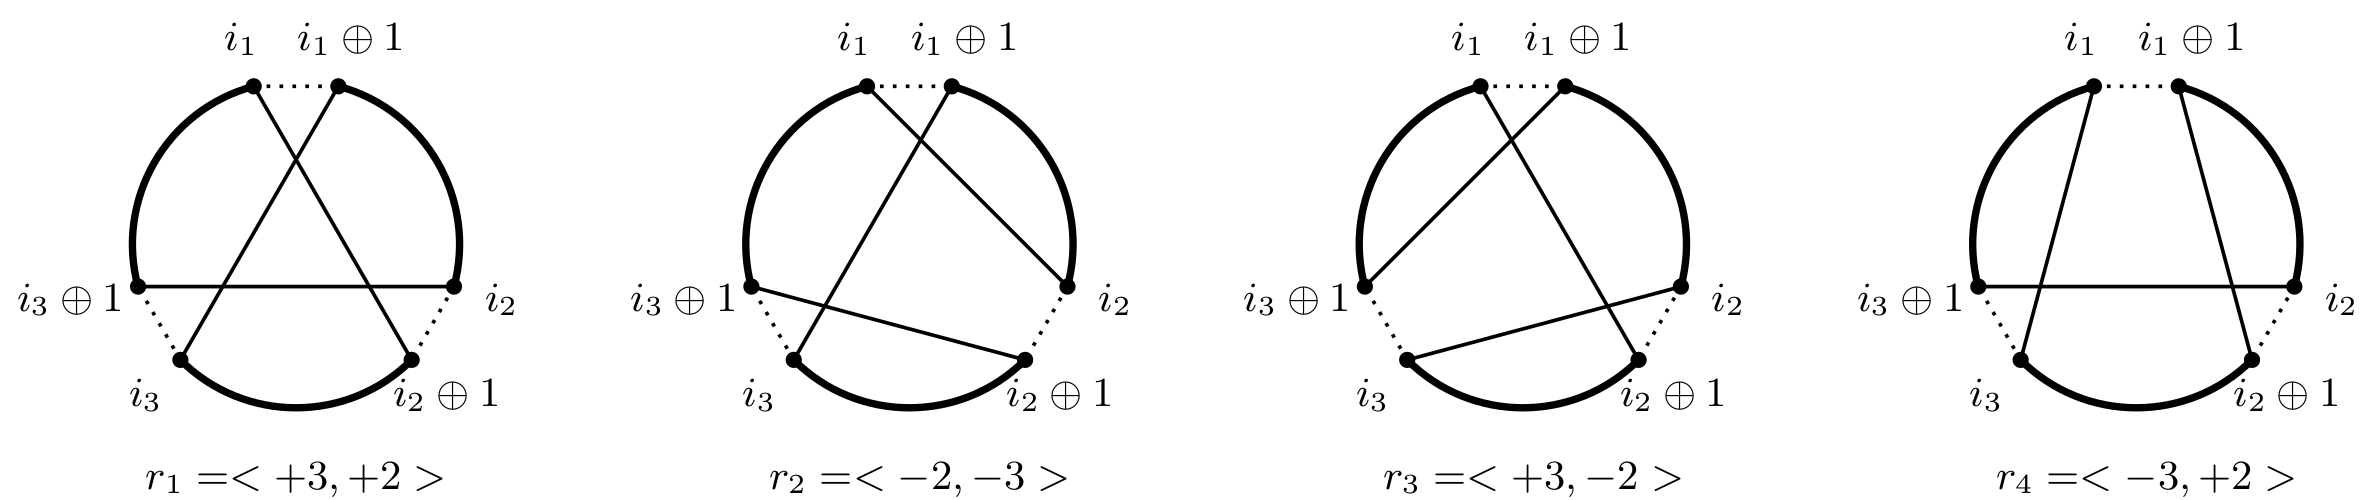
\includegraphics[width=400pt]{img/reinsertionSchemes.png}
    \caption{Una rappresentazione grafica degli schemi di reinserimenti. \textit{Fonte immagine \cite{3opt}}.}
\end{figure}

Consideriamo una selezione $S = (i_1, i_2, i_3)$, uno schema di reinserimenti $r$ e i rispettivi insiemi
$R(S)$ e $I(r)$. Allora, il guadagno della mossa $(R(S), I(r), 3)$ è $$\Delta{}(R, I) = w(R) - w(I)$$
In particolare, è possibile scomporre $\Delta$ come somma di tre funzioni di due parametri ciascuna:
$$\Delta{}(i_1,i_2,i_3) = f_1(i_1, i_2) + f_2(i_2, i_3) + f_3(i_1, i_3)$$

\newpage
Più precisamente, manipolando $\Delta$ per ogni schema di reinserimenti, si ottengono:


\begin{alignat*}{5}
    \langle+3,+2\rangle:& \qquad &f_1(x,y) &= \taup{x}{y} \qquad &f_2(x,y) &= \taup{x}{y} \qquad &f_3(x,y) &= \taup{y}{x} \\
    \langle-2,-3\rangle:& \qquad &f_1(x,y) &= \taup{x}{y\mns{}1} \qquad &f_2(x,y) &= \taum{x\pls{}1}{y\pls{}2} \qquad &f_3(x,y) &= \taup{y}{x} \\
    \langle+3,-2\rangle:& \qquad &f_1(x,y) &= \taup{x}{y} \qquad &f_2(x,y) &= \taup{x}{y\mns{}1} \qquad &f_3(x,y) &= \taum{y\pls{}1}{x\pls{}2} \\
    \langle-3,+2\rangle:& \qquad &f_1(x,y) &= \taum{x\pls{}1}{y\pls{}2} \qquad &f_2(x,y) &= \taup{x}{y} \qquad &f_3(x,y) &= \taup{y}{x\mns{}1} \\
\end{alignat*}
Dove $$dom(f_1) = \mathcal{S}_{12}, \qquad dom(f_2) = \mathcal{S}_{23}, \qquad dom(f_3) = \mathcal{S}_{13}$$

Fatte queste premesse, ci occuperemo ora di presentare l'idea descritta in \cite{3opt}.
L'assunzione che viene fatta è quella di supporre l'esistenza di un oracolo che, date due etichette $(a,b)$,
restituisca in tempo costante una coppia $(x,y) \in \mathcal{S}_{ab}$ che sia in una mossa 
\textit{best-improving}. In questo modo è necessaria
una scansione di costo lineare per trovare il ``terzo'' vertice della selezione che massimizzi $\Delta$.
L'obbiettivo è ora quello di simulare in modo efficiente l'oracolo: in particolare vogliamo restituire coppie
che appartengano ``molto probabilmente'' a una mossa \textit{best-improving}. Per fare ciò, l'osservazione chiave
è la seguente:
\begin{observation}[]
    Supponiamo di cercare la mossa \textit{best-improving}, di avere un ``campione''\\
    $S^*=(\overline{i_1}, \overline{i_2}, \overline{i_3})$ di costo $V = \Delta(S^*)$ e un
    candidato $S~=~(i_1,i_2,i_3)$. Allora, $\Delta(S) > \Delta(S^*)$ se e solo se
    $$\Bigg(f_1(i_1,i_2) > \frac{V}{3}\Bigg) \vee \Bigg(f_2(i_2,i_3) > \frac{V}{3}\Bigg) \vee \Bigg(f_3(i_1,i_3) > \frac{V}{3}\Bigg)$$
\end{observation}

Da questa semplice osservazione nasce l'idea di effettuare una ricerca in tre fasi: ad ogni fase 
$j \in \{1,2,3\}$ vengono enumerate le coppie che soddisfano il $j$-esimo disgiunto, dalla ``più promettente''
alla ``meno promettente'', terminando la fase appena la condizione non è più soddisfatta. La ricerca ``ordinata''
viene effettuata attraverso delle \textit{MaxHeap} e il valore $V$ viene aggiornato ogniqualvolta venga trovato
un nuovo ``campione''. Ad ogni passo, viene selezionata la coppia in cima alla heap e tramite una scansione
lineare si ricerca il terzo indice. Grazie alla combinazione tra l'organizzazione tramite heap e l'aggiornamento
online di $V$ si dimostra empiricamente che, in media, le selezioni considerate sono molte meno di $\Theta(n^3)$.
La procedura può essere descritta in questo modo:

\begin{algorithm}[H]
\caption{}
\begin{algorithmic}[1]
\Function{Modified3Opt}{$T, w$}
    \State $S^* \gets \varnothing,\quad r^* \gets \varnothing,\quad V \gets 0$
    \ForEach{$r \in Schemes$}
        \For{$j \gets 1,\; j \leq 3,\; j \gets j+1$}
            \State $H \gets \texttt{makeHeapWithBound}(V, j)$ \Comment Only pairs with gain $>\frac{V}{3}$
            \While{$|H|>0 \;\wedge\; \texttt{topPriority}(H) > \frac{V}{3}$}
                \State $\{x,y\} \gets \texttt{popElement}(H)$
                \State $z \gets \texttt{getZ}(x,y,j)$
                \State $\texttt{gain} \gets \texttt{getGain}(x,y,z,j)$
                \If{$V < \texttt{gain}$} \Comment Update gain information, best selection and best scheme
                    \State $V \gets \texttt{gain}$
                    \State $S^* \gets \{x,y,z\}$
                    \State $r^* \gets r$
                \EndIf
            \EndWhile
        \EndFor
    \EndFor
    \State $\texttt{apply}(T, S^*, r^*)$
\EndFunction
\end{algorithmic}
\end{algorithm}

% \begin{enumerate}
%     \item Si inizializzino $i:=1$, $j:=1$, $V:=0$, $S^*=\varnothing$, $r^*:=\varnothing$.
%     \item Si fissi lo schema $r:=r_i$.
%     \item Si costruisca la heap $H_j$ sulle coppie di $dom(f_j)$ che soddisfano la condizione $j$
%             dell'osservazione 2.1 e si inizializzi $V':=0$, $S:=\varnothing$.
%     \item Se $H_j$ non è vuota, si prenda la coppia $(x,y)$ in cima alla heap, e si scansionino
%             gli indici validi alla ricerca di $z$ che massimizzi $\Delta$ e si calcoli tale valore,
%             salvandolo in $V'$ e si imposti $S$ come la selezione data da $x,y,z$. Altrimenti si vada al
%             punto $6$.
%     \item Se $V'>V$ allora $V:=V'$, $S^*:=S$ e $r^*:=r$.
%     \item Se $j<3$ allora si incrementi $j:=j+1$ e si vada al punto $3$.
%     \item Se $i<4$ allora si incrementi $i:=i+1$ si vada al punto $2$.
%     \item Se $S^*\neq\varnothing$ si applichi la mossa $(R(S^*), I(r^*), 3)$.
% \end{enumerate}

\subsection{Lin-Kernighan}

Abbiamo considerato, nella sezione precedente, un approccio di tipo $k$-OPT: ad ogni passo,
un tour viene migliorato applicando $k$ rimozioni e $k$ reinserimenti (possibilmente non disgiunti).
Gli algoritmi di tipo $k$-OPT si basano sul concetto di:
\begin{definition}{\textbf{$k$-ottimalità}}
    Un tour viene definito $k$-ottimo se è impossibile ottenere un tour di costo minore
    applicando una mossa $k$-OPT.
\end{definition}

Dalla definizione è evidente che un tour $k$-ottimo sia anche $k'$-ottimo per $1\leq{}k'\leq{}k$ e che
un tour è ottimo se e solo se è $n$-ottimo. Da queste osservazioni si evince che, generalmente, più
$k$ è elevato e migliore sarà la precisione dell'algoritmo. Sfortunatamente, il numero di mosse 
$k$-OPT esplode al crescere di $k$ ed è quindi necessario scegliere un $k$ non troppo elevato. Un ulteriore
svantaggio è il fatto di dover specificare in anticipo il valore di $k$ anche se non è noto a priori il 
migliore compromesso tra il tempo di esecuzione e la bontà dell'approssimazione per un fissato $k$ su un 
preciso grafo.

L'idea di Lin e Kernighan è stata quella di effettuare ``online'' la scelta di $k$: ad ogni step, 
l'algoritmo esamina una mossa $k$-OPT per valori crescenti di $k$ finché non viene raggiunta una condizione 
di terminazione. Più precisamente, ad ogni step l'algoritmo cerca di trovare due insiemi di archi 
$X = \{x_1,\dots,x_k\}$ e $Y = \{y_1,\dots,y_k\}$ tali che il tour ottenuto eliminando gli archi 
di $X$ e aggiungendo gli archi di $Y$ sia ancora valido. I due insiemi vengono costruiti elemento per elemento.
Inizialmente $X$ e $Y$ sono vuoti; al passo $i$ vengono aggiunti $x_i$ e $y_i$ rispettivamente a $X$ e $Y$.
\ \\

Prima di proseguire dimostriamo questo semplice fatto:
\begin{theorem}
    Sia $(a_1, a_2, \dots, a_m)$ una sequenza di interi tale che $a_1+a_2+\dots+a_m > 0$. Allora, esiste
    una permutazione ciclica $\sigma$ tale che, per ogni $1\leq{}i\leq{}m$, $a_{\sigma(1)}+\dots+a_{\sigma(i)} > 0$.
\end{theorem}

\begin{proof}{\textit{(Per induzione su $m\ge$1)}}\\
    \textbf{Base:} se $m=1$, $\sigma$ è la permutazione identica $id_1$.\\
    \textbf{Step:} sia $m>1$ e si considerino i seguenti casi:
    \begin{itemize}
        \item se $a_1+\dots+a_{m-1}>0$ allora, per ipotesi induttiva, esiste una
                permutazione ciclica $\tau$ tale che $a_{\tau(1)}+\dots+a_{\tau(i)} > 0$ per
                ogni $1\leq{}i\leq{m-1}$. Ma allora $\sigma = \tau{}\circ{}id_m$.

        \item altrimenti, sappiamo che $|a_1+\dots+a_{m-1}| < a_m$, sia quindi $\tau=(2,3,\dots,m,1)$, ovvero
                la sequenza $(a_m,a_1,a_2,\dots,a_{m-1})$. Ma allora tale sequenza ricade nel caso precedente,
                per cui esiste una permutazione $\sigma'$ che soddisfa il teorema. Da cui $\sigma=\sigma'\circ\tau$.
    \end{itemize}
\end{proof}
\ \\

Per rendere efficiente la costruzione di $X$ e $Y$, gli archi che vengono scelti devono rispettare alcuni criteri:
\begin{description}
    \item[1. Scambio sequenziale:] $x_i, y_i, x_{i+1}$ devono condividere un vertice; più precisamente, vale 
                $x_i=(t_{2i-1}, t_{2i}), \\y_i=(t_{2i}, t_{2i+1}),\;\; x_{i+1}=(t_{2i+1},t_{2i+2})$ dove $t_i$ indica
                l'$i$-esimo vertice del tour dopo che è stato effettuato lo scambio $X, Y$.

    \item[2. Fattibilità:] viene richiesto che $x_i=(t_{2i-1}, t_{2i})$ venga scelto in modo tale che se
                viene scelto $y_i = (t_{2i}, t_1)$, il tour risultante sia valido. In questo modo viene 
                garantita la possibilità di chiudere il tour in ogni momento, riducendo così il tempo di 
                esecuzione e semplificando il codice. 

    \item[3. Guadagno positivo:] detti $g_i = w(x_i)-w(y_i)$ e $G_i = \displaystyle\sum_{i=1}^{i}{g_i}$, viene 
                richiesto $G_i>0$ per ogni $i$. Questo criterio pone una condizione di terminazione molto 
                efficace nella pratica e, sebbene sembri troppo restrittivo, non lo è affatto in virtù del 
                Teorema 2.2.1.

    \item[4. Disgiuntività:] viene richiesto che, ad ogni passo, $X\cap{}Y\neq\varnothing$; il criterio 
                semplifica ulteriormente il codice e fornisce un'altra condizione di terminazione. 
\end{description}

L'algoritmo (semplificato) viene quindi schematizzato come segue:

\begin{algorithm}[H]
\caption{}
\begin{enumerate}
    \item Si generi un tour $T$ casualmente.
    \item Si inizializzi $i:=1$. Si Scelga $t_1$.
    \item Si scelga $x_1=(t_1,t_2) \in T$.
    \item Si scelga $y_1=(t_2, t_3) \notin T$ tale che $G_1>0$. Se ciò non è possibile, si proceda al passo $12$.
    \item Sia $i:=i+1$.
    \item Si scelga $x_i=(t_{2i-1}, t_{2i}) \in T$ tale che:\\
            (a) Se $t_{2i}$ viene connesso a $t_1$, il risultato deve essere un tour valido $T'$;\\
            (b) $x_i\neq{}y_s$ per ogni $s<i$;\\
          Se $w(T') < w(T)$ si salvi $T:=T'$ e si ritorni al passo $2$.
    \item Si scelga $y_i=(t_{2i}, t_{2i+1}) \notin T$ tale che:\\
            (a) $G_i>0$;\\
            (b) $y_i\neq{}x_s$ per ogni $s\leq{}i$;\\
            (c) $x_{i+1}$ esiste;\\
          Se tale $y_i$ esiste, si ritorni al passo $5$.
    \item Se c'è un'alternativa non provata per $y_2$, si imposti $i:=2$ e si ritorni al passo $7$.
    \item Se c'è un'alternativa non provata per $x_2$, si imposti $i:=2$ e si ritorni al passo $6$.
    \item Se c'è un'alternativa non provata per $y_1$, si imposti $i:=1$ e si ritorni al passo $4$.
    \item Se c'è un'alternativa non provata per $x_1$, si imposti $i:=1$ e si ritorni al passo $3$.
    \item Se c'è un'alternativa non provata per $t_1$, si ritorni al passo $2$.
    \item Stop.
\end{enumerate}
\end{algorithm}

Ai passi $6$ e $7$, l'algoritmo controlla se le scelte per $x_i$ e $y_i$ soddisfino i criteri;
l'algoritmo originale, tuttavia, permette di indagare più a fondo le scelte che possono essere fatte
per $i=2$: per alcuni casi è infatti possibile non rispettare, temporaneamente, il criterio di
\textbf{fattibilità} per ottenere successivamente un tour valido. Lo schema descritto è più semplice anche
per quanto riguarda il passo $6$: $T$ viene rimpiazzato da $T'$ appena quest'ultimo ha un costo inferiore;
l'algoritmo originale, invece, continua ad aggiungere potenziali scambi con lo scopo di trovare un tour 
ancora più vantaggioso, rimpiazzando $T$ con il tour con costo migliore trovato. Questa scelta, tuttavia,
non produce tour migliori, non migliora il tempo di esecuzione e complica notevolmente il codice\cite{LKH}.\\

Per migliorare le prestazioni dell'algoritmo sono stati aggiunte altre regole con lo scopo di 
\textit{limitare} e \textit{indirizzare} la scelta dei possibili archi da rimuovere o aggiungere:
\begin{enumerate}
    \setcounter{enumi}{4}
    \item[\textbf{5.}] La ricerca di un arco $y_i=(t_{2i},t_{2i+1})$ viene limitata ai $5$ archi di costo minore
            adiacen ti a $t_{2i}$.
    \item[\textbf{6.}] Per $i\geq{}4$ non possono essere rimossi archi che appartengono a tutti i $2-5$
            tour migliori.
    \item[\textbf{7.}] La ricerca viene interrotta se il tour corrente è lo stesso di quello trovato all'interazione
            precedente.
    \item[\textbf{8.}] Se vi sono più scelte per $y_i (i\geq{}2)$, viene data una priorità $w(x_{i+1})-w(y_i)$.
    \item[\textbf{9.}] Se vi sono due alternative per $x_4$, viene data priorità a quella con costo maggiore.
\end{enumerate}

Come ultima euristica, al termine degli step ``sequenziali'', vengono effettuate mosse $4$-OPT non sequenziali
con lo scopo di ottenere ulteriori miglioramenti.

\section{Euristiche composite e la variante di Helsgaun dell'algoritmo Lin-Kernighan}

Come ultima classe di euristiche vengono presentate le cosiddette \textit{composite} che cercano di ``combinare''
i vantaggi di entrambe le altre classi. A titolo di esempio verrà descritto l'algoritmo Lin-Kernighan-Helsgaun.\\

In \cite{LKH} viene presentata un'implementazione efficace ispirata all'algoritmo di Lin e Kernighan.
Sebbene la procedura si basi sempre sull'idea di applicare mosse $k$-OPT determinando $k$ ``al volo'', la 
variante presentata da Helsgaun applica alcune modifiche riguardo alla scelta dei ``vicini'' da esaminare:
se in \cite{LK} vengono esaminati i cinque archi incidenti meno costosi (regola $5$), nel nuovo algoritmo
è centrale il concetto di \textit{insieme dei candidati} che migliora notevolmente la regola $5$. Inoltre,
se in \cite{LK} le ``mosse base'' (ovvero la \textit{profondità} con cui l'algoritmo esamina le scelte che
non rispettano il criterio di \textbf{fattibilità}) sono $2/3$-OPT, nel nuovo algoritmo vengono estese a mosse 
$5$-OPT.

\subsection{Insieme dei candidati e $\alpha$-nearness}

Prima di proseguire, diamo le seguenti definizioni.
\begin{definition}[\textbf{$1$-Tree}]
    Sia $G$ un grafo e $T$ uno Spanning Tree su $G\setminus{}\{1\}$. Siano inoltre $e_1, e_2$ due archi 
    di $G$ incidenti in $1$. Diremo allora che $T_1 := T\cup{}\{e_1, e_2\}$ è un $1$-Tree per $G$.\\
    Diremo inoltre che $T_1$ è un \textbf{$1$-Tree Minimo} (\textit{Minimum $1$-Tree} oppure M$1$T) se non 
    esiste un altro $1$-Tree di peso minore.
\end{definition}

\begin{observation}
    Un tour ottimo è un $1$-Tree Minimo tra quelli in cui ogni vertice ha grado $2$.
\end{observation}

\begin{observation}
    Se un $1$-Tree Minimo è un tour, allora è un tour ottimo.
\end{observation}
\ \\
È quindi possibile riformulare il TSP come:
\begin{definition}[\textbf{TSP su 1-Tree}]
    Sia $G$ un grafo pesato e completo. Determinare un $1$-Tree Minimo di $G$ tra quelli che hanno ogni vertice 
    di grado $2$.
\end{definition}

\begin{figure}[H]
    \centering
    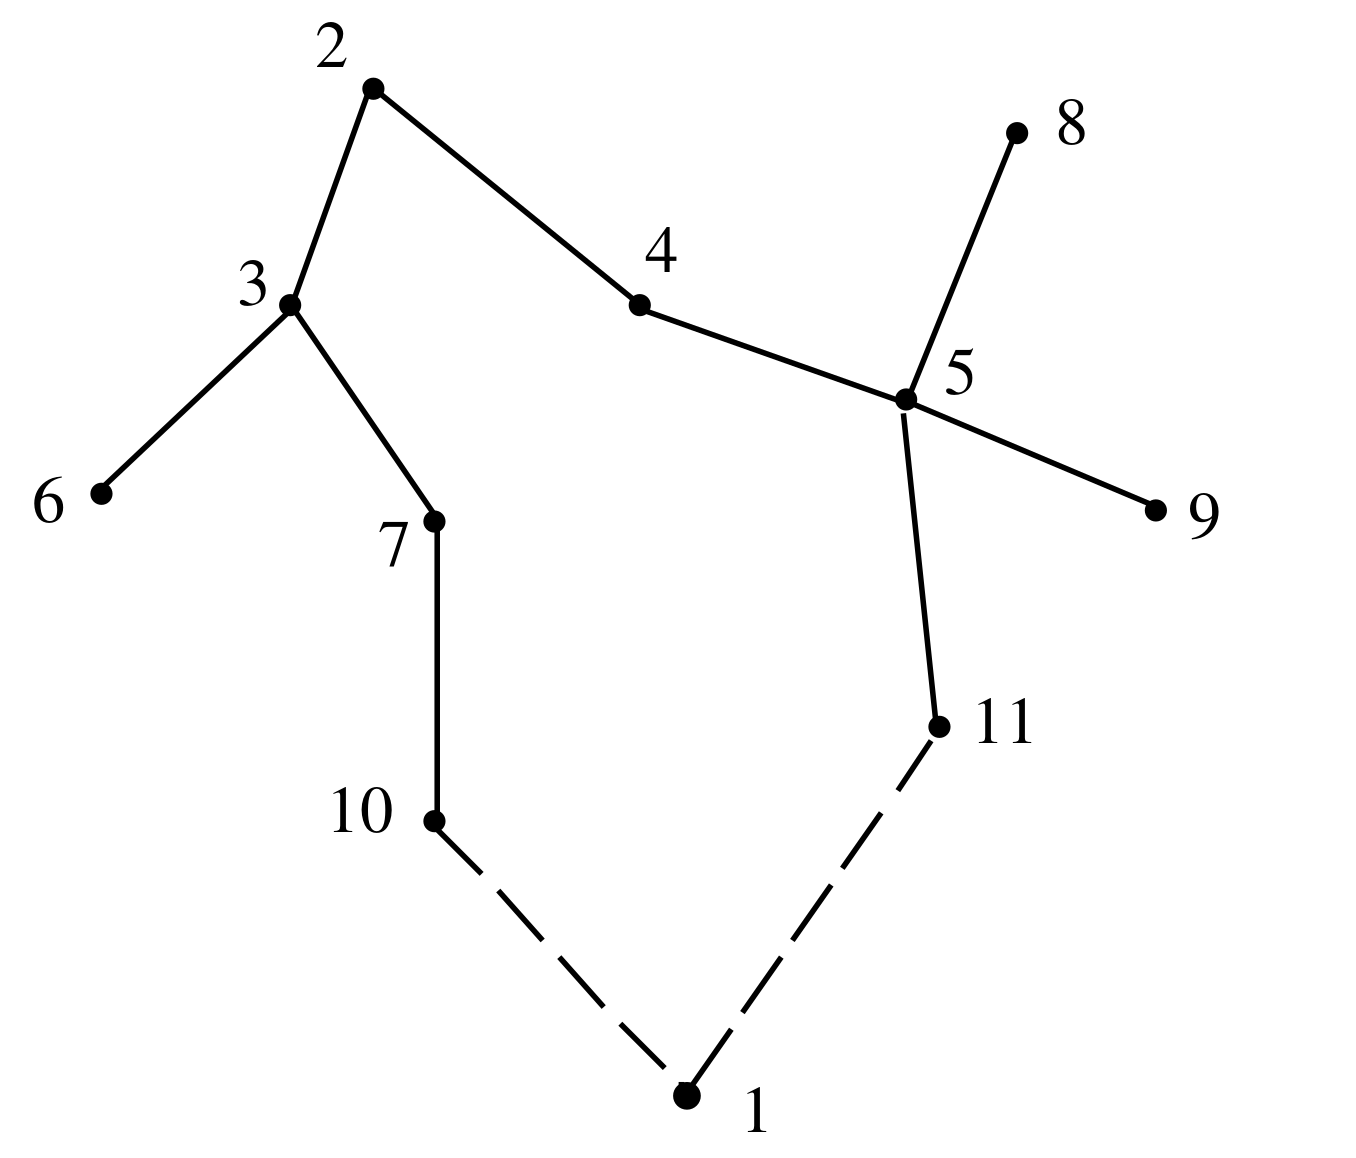
\includegraphics[width=250pt]{img/1Tree.png}
    \caption{Un $1$-Tree. \textit{Fonte immagine \cite{LKH}}}
\end{figure}

Come già accennato, nel nuovo algoritmo è fondamentale il ruolo di \textit{insieme dei candidati} che 
estende e migliora la regola $5$ di \cite{LK}. Tale regola si basa sull'idea (troppo restrittiva) che la 
probabilità che un arco appartenga al tour ottimo cresca al diminuire del costo dello stesso. Una misura migliore 
sembra essere, invece, l'appartenenza o meno a un Minimum $1$-Tree: risulta infatti che, in media, un arco 
appartente ad un M$1$T abbia probabilità $0.7\sim0.8$ di appartenere a un tour ottimo \cite{LKH}. L'idea è quindi quella di 
costruire l'insieme dei candidati a partire da una misura di ``vicinanza'' a un M$1$T.

\begin{definition}[\textbf{$\alpha$-nearness}]
    Sia $T_1$ un Minimum $1$-Tree di peso $w(T_1)$ e sia $T_1^+(i, j)$ il Minimum $1$-Tree di $G$ che contiene 
    l'arco $(i, j)$. Definiamo quindi la $\alpha$-nearness di (i, j) come
    $$\alpha(i, j) := w(T_1^+(i,j)) - w(T_1)$$
\end{definition}
\ \\
Esaminiamo due semplici proprietà di $\alpha$.
\begin{theorem}\ \\
    (1) $\alpha(i,j) \geq 0$ per ogni arco $(i, j)$.\\
    (2) Se $(i, j)$ appartiene a qualche M$1$T, allora $\alpha(i,j)=0$.
\end{theorem}

\begin{proof}\ \\
    (1) $\alpha(i,j) = w(T_1^+(i,j))-w(T_1) \geq w(T_1)-w(T_1) = 0$.\\
    (2) $\alpha(i,j) = w(T_1^+(i,j))-w(T_1) = w(T_1)-w(T_1) = 0$.
\end{proof}
\ \\
La prima difficoltà si presenta nel calcolo della $\alpha$-nearness per ogni arco del grafo: dalla definizione 
sembra necessario, ogni volta, aggiungere l'arco $(i,j)$ a un M$1$T ed eliminare l'ipotetico ciclo che si 
verrebbe a formare nel caso in cui $(i.j)$ non sia già presente in $T_1$. Tale operazione ha costo $\mathcal{O}(n)$ 
per ogni arco del grafo, per un costo totale di $\mathcal{O}(n^3)$ per computare tutte le $\alpha$. L'osservazione 
chiave è la seguente.

\begin{observation}
    Sia $\beta(i,j)$ il costo dell'arco da rimuovere (\textit{i.e. il più costoso}) se, all'inserimento di $(i,j)$,
    si forma un ciclo. Ne segue che $\alpha(i,j)=w(i,j)-\beta(i,j)$. Si considerino quindi $i$ e $(j_1,j_2)$ 
    tale che $j_1$ si trovi nel ciclo formatosi all'aggiunta dell'arco $(i,j_2)$. Allora 
    $$\beta(i,j_2) = \max\{\beta(i,j_1), w(j_1,j_2)\}$$
\end{observation}
\ \\
Da questa osservazione è possibile calcolare, in tempo ottimale $\Theta(n^2)$, le $\alpha$ di tutti gli archi del 
grafo. L'algoritmo sfrutta la programmazione dinamica e assume che i vertici siano ordinati topologicamente rispetto 
alla relazione ``discendente'' venutasi a creare durante la costruzione dell'M$1$T (ad esempio con Prim).

\begin{algorithm}[H]
\caption{}
\begin{algorithmic}
\Require{$dad(i)=j \;\Longrightarrow\; i<j$}
\Function{ComputeBeta}{$ $}
    \State $\beta \gets \texttt{new Matrix}(n, n)$
    \For{$i \gets 2,\; i < n,\; i \gets i+1$}
        \State $\beta[i][i] \gets -\infty$
        \For{$j \gets i+1,\; j \leq n,\; j \gets j+1$}
            \State $\beta[i][j] \gets \max\big\{\beta[i][dad(j)],\; w(j, dad(j))\big\}$
            \State $\beta[j][i] \gets \beta[i][j]$
        \EndFor
    \EndFor
\EndFunction
\end{algorithmic}
\end{algorithm}

Sebbene l'algoritmo necessiti di spazio quadratico per la matrice $\beta$, è possibile modificarlo 
in modo da richiedere solo spazio lineare e riuscire in ogni caso a calcolare tutti gli $\alpha$ \cite{LKH}.
Tale pseudocodice viene omesso.

\ \\
Nonostante gli $\alpha$ siano migliori rispetto al semplice costo per definire la regola $5$, è possibile 
migliorare ulteriormente il loro effetto applicando delle trasformazioni ai pesi degli archi del grafo.
\begin{observation}
    Ogni tour è un $1$-Tree, quindi $w(T_1)$ è una limitazione inferiore al costo del tour ottimo.
\end{observation}
\begin{observation}
    Se il peso di tutti gli archi adiacenti a $v_i$ viene incrementato dello stesso valore $\pi_i$, un 
    tour che era precedentemente ottimo lo è ancora. Inoltre, se $T_{\pi}$ è un M$1$T sul grafo perturbato 
    $G_{\pi}$, vale $$w(T_{\pi}) - 2\displaystyle\sum_{i=1}^{n}{\pi_i} \leq w(T_{OPT})$$.
\end{observation}
\begin{observation}
    Dalle osservazioni precedenti si ottiene che il valore $f(\pi) = w(T_{\pi}) - 2\displaystyle\sum_{i=1}^{n}{\pi_i}$ 
    è ancora una limitazione inferiore al tour ottimo per $G$.
\end{observation}
\ \\
L'attenzione viene quindi spostata sulla ricerca della perturbazione $\pi$ che massimizzi $f(\pi)$. Tale 
massimizzazione è nota come limitazione di Held-Karp.

La strategia per stimare la perturbazione ottima è nota come ``ottimizzazione del subgradiente'' e l'idea 
è quella di, iterativamente, considerare il subgradiente di $f$ ed effettuare un ``passo'' nel suo verso. 
Si può dimostrare che, in questo caso, un subgradiente per $f$ è $v := deg - \mathbf{2}$, dove $deg$ è il 
vettore dei gradi dei vertici in $T_{\pi}$ e $\mathbf{2}$ è un vettore di soli $2$. L'idea è quella di rendere 
più corti gli archi incidenti a vertici di grado $1$, più lunghi quelli incidenti a vertici di grado maggiore 
di $2$ e di non cambiare quelli incidenti a vertici di grado esattamente $2$: in questo modo, si costringe 
$T_{\pi}$ ad ``alleggerire'' i vertici con troppi archi adiacenti e ad ``appesantire'' i vertici di grado $1$,
nella speranza di ottenere un tour. Infatti, in virtù dell'osservazione 2.3.2, se $T_{\pi}$ è un tour allora è 
un tour ottimo.

La procedura iterativa viene così schematizzata:

\begin{algorithm}[H]
\caption{}
\begin{algorithmic}[1]
\Function{ascent}{$ $}
    \State $\pi \gets \mathbf{0}$
    \State $F \gets -\infty$
    \State $k \gets 0$
    \Repeat
        \State $T_{\pi} \gets \texttt{getMin1Tree}(\pi)$
        \State $f \gets w(T_{\pi})$
        \For{$i \gets 1,\; i \leq n,\; i \gets k+1$}
            \State $f \gets f - 2\pi[i]$
        \EndFor
        \State $F \gets \max\{F, f\}$
        \State $v \gets deg(T_{\pi}) - \mathbf{2}$
        \If{$\norm{v} = 0$}
            \State \Return $F$
        \EndIf
        \State $t \gets \texttt{getStepSize}(k)$
        \State $\pi \gets \pi + tv$
        \State $k \gets k+1$
    \Until{$\texttt{exitCondition} = \texttt{True}$}
    \State \Return $F$
\EndFunction
\end{algorithmic}
\end{algorithm}
% 
% \begin{enumerate}
%     \item Sia $k:=0$, $\pi_0:=\mathbf{0}$ e $F = -\infty$.
%     \item Si costruisca un M$1$T $T_{\pi_k}$.
%     \item Si calcoli $f(\pi_k) = w(T_{\pi_k}) - 2\displaystyle\sum_{i=1}^{n}{\pi_k(i)}$.
%     \item Sia $F := \max\{F, f(\pi_k)\}$.
%     \item Sia $v_k := deg_k - \mathbf{2}$, dove $deg_k$ contiene i gradi dei vertici di $T_{\pi_k}$.
%     \item Se $\norm{v_k} = 0$, allora $T_{\pi_k}$ è un tour ottimo. Stop.
%     \item Se viene raggiunta una condizione di terminazione, stop.
%     \item Si scelga la dimensione del passo $t_k$.
%     \item Si consideri $\pi_{k+1} := \pi_k + t_kv_k$.
%     \item Si incrementi $k := k+1$ e si ritorni al passo $2$.
% \end{enumerate}
\ \\
La convergenza del metodo alla limitazione di Held-Karp è assicurata se $\displaystyle\lim_{k\to\infty}{t_k}=0$ e 
$\displaystyle\sum_{k=0}^{\infty}{t_k} = \infty$~\cite{subgr}. Tuttavia, anche se la convergenza è assicurata
(\textit{ad esempio per $t_k:=\frac{t_0}{k}$}), è necessario che sia veloce. Vi sono molteplici strategie che 
sono efficaci nella pratica, tuttavia dipendono dal grafo che si sta considerando. Helsgaun propone la 
seguente:
\begin{itemize}
    \item La dimensione del passo rimane costante per ogni ``periodo''.
    \item Quando un periodo termina, viene dimezzato.
    \item La lunghezza del primo periodo viene impostata a $\frac{n}{2}$.
    \item $t_0 := 1$ e, durante il primo periodo, viene raddoppiato ad ogni step fintantoché $F$ non 
            viene incrementato.
    \item Se l'ultimo step di un periodo incrementa $F$, allora viene raddoppiato.
    \item L'algoritmo termina se $v_k = \mathbf{0}$ oppure il periodo o il passo diventano 0.
\end{itemize}

Una volta trovata la perturbazione $\pi$ viene calcolato il nuovo valore di ``vicinanza migliorata'' che 
denoteremo con $\alpha_{\pi}$.

\subsection{La scelta del tour iniziale}

L'algoritmo Lin-Kernighan applica molteplici scambi sullo stesso problema, utilizzando ad ogni 
iterazione un tour generato casualmente. Helsgaun, invece, sfrutta un'euristica di tipo 
``tour construction'':
\begin{algorithm}[H]
\caption{}
\begin{enumerate}
    \item Si scelga un vertice $i$ casualmente.
    \item Si scelga un vertice $j$, non ancora scelto, nel modo seguente:
    \begin{enumerate}
        \item Se possibile, si scelga $j$ tale che:
        \begin{enumerate}
            \item $(i,j)$ è un ``candidato''
            \item $\alpha(i,j)=0$
            \item $(i,j)$ appartiene al migliore tour trovato fin'ora
        \end{enumerate}
        \item Altrimenti, si scelga $j$ tale che $(i,j)$ sia un ``candidato''.
        \item Altrimenti, si scelga $j$ casualmente.
    \end{enumerate}
    \item Sia $i:=j$, se vi sono ancora vertici da scegliere, si ritorni al passo $2$.
\end{enumerate}
\end{algorithm}

% Implementazione e testing
\chapter{Implementazione e testing}

A seguito di una trattazione teorica è seguita un'attività sperimentale atta a confrontare le euristiche 
studiate. La sperimentazione si è ispirata alla competizione ``DIMACS Implementation Challenge'' svoltasi 
nel $2000$, durante la quale sono state messe a confronto diverse euristiche sviluppate e implementate da 
ricercatori di ogni parte del mondo \cite{STSP}. Gli algoritmi sono stati testati sia su una serie di grafi 
generati casualmente, sia su una serie di grafi presenti in TSPLIB \cite{tsplib}.

\section{Scelte implementative}

L'implementazione delle euristiche e dei programmi di misurazione è stata svolta nel linguaggio \texttt{C++}: la 
scelta è dovuta alla flessibilità con cui il linguaggio permette l'astrazione pur mantenendo elevate prestazioni.
Di seguito verranno descritte, per ogni euristica, le strutture dati utilizzate e le scelte effettuate.

\subsection{Strutture dati comuni e ridefinizioni di tipo}

Le entità principali del problema sono il ``Tour'' e il ``Grafo''. Per quanto riguarda il Tour è stato 
deciso di utilizzare la classe \texttt{std::vector}, fornito dalla libreria standard del 
linguaggio. Il vantaggio principale di \texttt{std::vector} è il fatto di rappresentare un array 
ridimensionabile che fornisce sia l'accesso diretto ad un elemento (tramite indice), sia il ``push'' 
di un elemento in coda ad esso, entrambi con complessità $\mathcal{O}(1)$\footnote{Più precisamente, il 
\texttt{push\_back} ha complessità costante \textit{ammortizzata}: \texttt{std::vector} possiede una 
``capacità'' iniziale (un buffer interno allocato dinamicamente) e ogniqualvolta che un elemento deve essere 
``pushato'' ma il buffer è pieno, \texttt{std::vector} alloca un nuovo buffer di dimensione doppia; è facile 
notare come l'inserimento di $n$ elementi abbia quindi complessità $\mathcal{O}(n).$}. Queste performance sono 
quindi adatte per la gestione dei tour negli algoritmi ``tour construction''. Il Grafo in input,
invece, è stato rappresentato come matrice dei costi.

È stato fatto uso estensivo della keyword \texttt{typedef} per rendere più espressivo il codice: in questo modo,
semplici \texttt{double}, \texttt{int} o \texttt{std::vector<int>} vengono utilizzati come \texttt{Cost}, 
\texttt{Vertex} o \texttt{Tour}.

\subsection{Nearest Neighbor e Nearest Insertion}

È stato deciso di mantenere la semplicità concettuale delle due euristiche anche nell'implementazione: 
ad ogni passo vengono scansionati tutti i vertici alla ricerca del ``migliore'' libero, 
per poi aggiungerlo al tour parziale a seconda della politica di inserimento. Solo per quanto riguarda 
Nearest Insertion si è deciso di utilizzare una struttura dati di supporto, adatta agli inserimenti in 
posizioni arbitrarie della stessa: \texttt{std::list<>}. Anche in questo caso la classe viene 
offerta dalla libreria standard e rappresenta una lista concatenata. Il \texttt{typedef} utilizzato è 
\texttt{TourList}.

\subsection{Christofides}

L'algoritmo di Christofides richiede la costruzione di un Minimum Spanning Tree e di un Minimum Weight 
Matching. Per quanto riguarda l'MST si è deciso di utilizzare l'algoritmo di Prim, che è stato implementato 
senza l'uso di strutture dati particolari: la scelta è dovuta al fatto che, dovendo considerare solo grafi 
completi, l'utilizzo di Code con Priorità o algoritmi alternativi non avrebbe garantito prestazioni migliori. 
La costruzione del Minimum Weight Matching è stata invece semplificata: la strategia utilizzata è di tipo 
\textit{greedy} nel senso che vengono scansionati gli archi in ordine crescente di peso e viene scelto 
il primo incidente a due vertici non ancora aggiunti al matching. Infine, la ricerca del circuito 
euleriano è stata svolta ricorsivamente, modificando il classico algoritmo \textit{Depth First Search}: 
l'esistenza del circuito è assicurata dal Teorema 2.1.2 quindi è sufficiente visitare in profondità ogni arco non ancora 
visitato; dovendo effettuare inserimenti di vertici in posizioni arbitrarie del circuito che si sta 
costruendo, si è deciso di sfruttare \texttt{TourList}. Inoltre, avendo rappresentato gli archi non 
diretti del grafo come una coppia di archi diretti nei due versi opposti, sono state associate delle 
etichette in modo da riuscire a ricavarne una dall'altra. In questo modo è possibile ``visitare'' entrambi 
i versi di un arco che si sta per percorrere.\\

\begin{figure}[H]
    \centering
    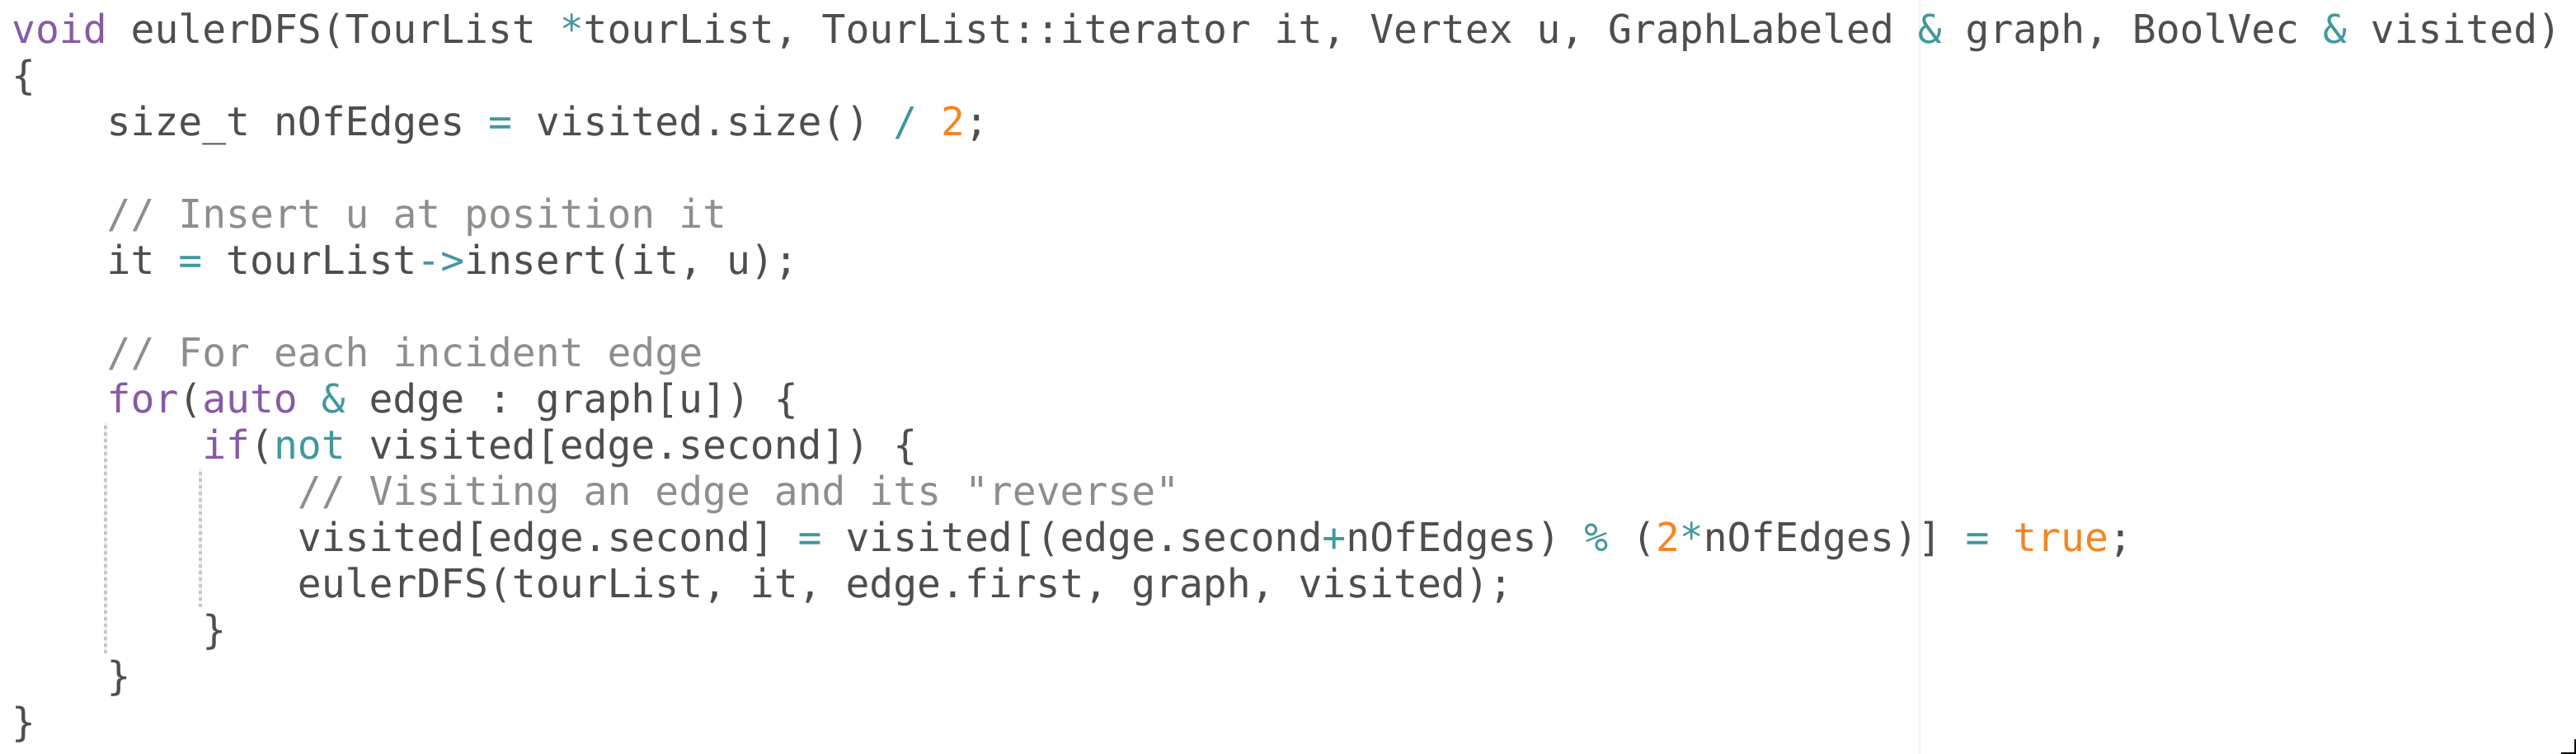
\includegraphics[width=450pt]{img/eulerDFS.png}
    \caption{Il codice per la ricerca del circuito euleriano.}
\end{figure}

\subsection{3-OPT}

L'implementazione scelta è quella descritta in \cite{3opt}. Si è mantenuta la scelta di utilizzare 
\texttt{std::vector} per rappresentare un Tour. Le MaxHeap, invece, sono state implementate sfruttando 
la classe \texttt{std::priority\_queue} fornita dalla libreria standard: è stato, tuttavia, definito il 
tipo di dato \texttt{HeapElement} dotato di operatore di confronto, così da rendere agevole l'utilizzo 
della coda. L'applicazione della mossa 3-OPT trovata viene fatta seguendo la costruzione a ``segmenti'' 
definita dallo \textit{schemda di reinserimento}: per evitare situazioni limite (segmenti che sono a cavallo 
tra inizio e fine del tour) è stato deciso di raddoppiare il circuito, così da ``simulare'', attraverso il 
\texttt{vector}, la ciclicità. È stata utilizzata la funzione \texttt{std::reverse()} per capovolgere i 
segmenti che vengono percorsi in senso antiorario: il tour viene quindi costruito accodando i diversi 
segmenti con l'orientamento definito dallo schema.
\ \\

\begin{figure}[H]
    \centering
    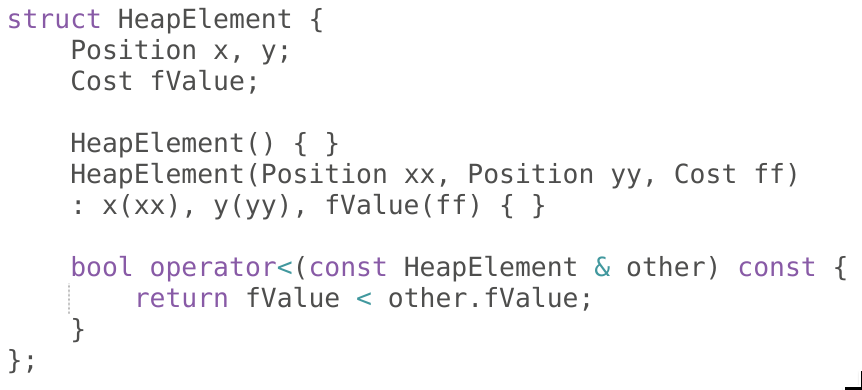
\includegraphics[width=250pt]{img/HeapElement.png}
    \caption{Il tipo di dato HeapElement.}
\end{figure}
\ \\
Sono state sviluppate tre varianti di 3-OPT:
\begin{description}
    \item[\texttt{random3opt}:] il tour iniziale viene generato casualmente.
    \item[\texttt{christofides3opt}:] il tour iniziale viene generato con l'algoritmo \texttt{CHR}.
    \item[\texttt{reiterated3opt}:] inizialmente il tour viene generato con \texttt{CHR}; quando viene 
            trovato un minimo locale, il tour viene ``perturbato'' scambiando casualmente alcuni vertici.
            La procedura quindi viene eseguita a partire da questo tour perturbato; la scelta di quanti 
            vertici scambiare e di quante volte reiterare viene decisa parametricamente: in particolare,
            viene mantenuto un parametro \texttt{maxIteration} che viene incrementato ogni volta che 
            viene prodotto un minimo locale migliore dei precedenti e la procedura termina quando vengono 
            eseguite \texttt{maxIteration} iterazioni.   
\end{description}

\subsection{Lin-Kernighan-Helsgaun (\texttt{LKH})}

A causa della complessità implementativa di questo algoritmo è stato deciso di seguire l'approccio 
descritto in \cite{LKH}: il tour viene rappresentato come una lista concatenata di elementi di tipo 
\texttt{LKHNode}. Come nel caso di Christofides, si è deciso di semplificare l'algoritmo rispetto a quello 
ufficiale: il tour iniziale non viene generato con l'euristica costruttiva di 
Helsgaun ma con \texttt{CHR}; questa scelta viene giustificata in \cite{LKH}. Un'altra scelta 
discordante con l'algoritmo di Helsgaun è nelle ``mosse base'': in \cite{LKH} vengono utilizzate mosse 
sequenziali 5-OPT; si è deciso invece di utilizzare mosse sequenziali 3-OPT per favorire la leggibilità 
del codice pur mantenendo la struttura originale dell'algoritmo. 

La procedura, come descritta da Helsgaun, costruisce gli \textit{insiemi dei candidati} 
basandosi sulla nozione di $\alpha$-nearness migliorata. Questa viene calcolata da un 
M$1$T del grafo perturbato, massimizzando $\pi$ con il metodo del subgradiente (nel codice, \texttt{ascent}).
\ \\

\begin{figure}[H]
    \centering
    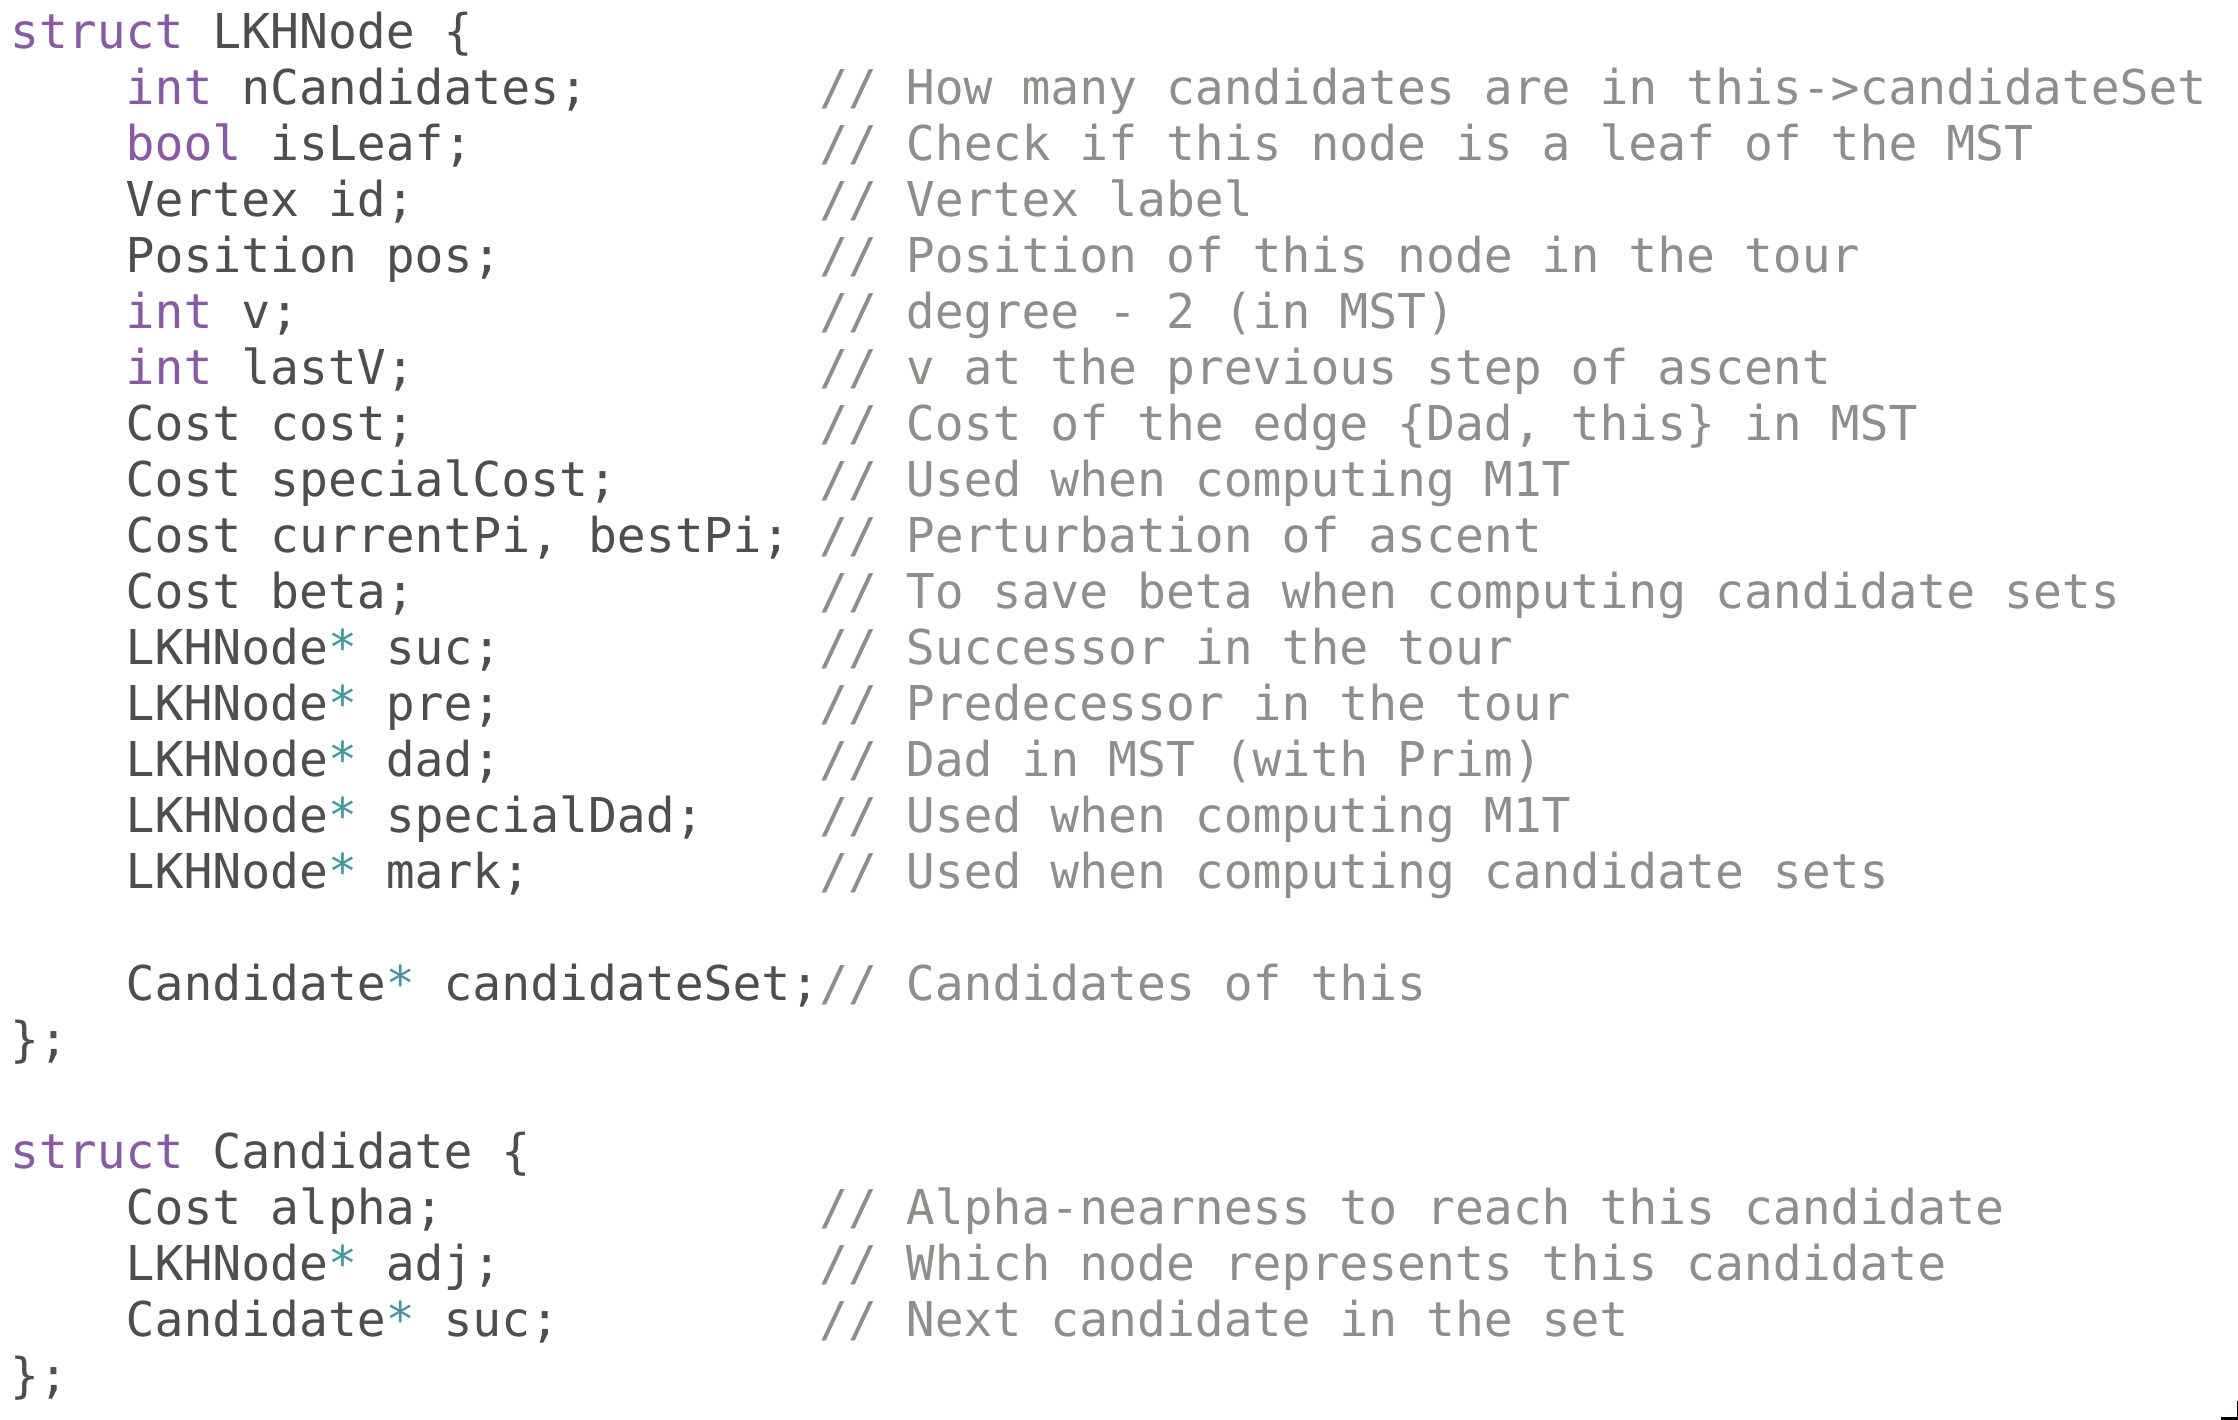
\includegraphics[width=350pt]{img/LKHNode.png}
    \caption{Tipi di dato \texttt{LKHNode} e \texttt{Candidate}.}
\end{figure}


Una volta generati i candidati vengono effettuate \texttt{maxRuns} iterazioni: ad ogni iterazione viene generato 
un tour con \texttt{CHR} e per \texttt{maxTrials} iterazioni viene eseguito \texttt{linKernighan} su tale tour. Al termine 
di ogni ``trial'', se si è trovato un tour migliore dei precedenti, i candidati vengono modificati inserendo 
gli archi del tour migliorato. Al termine di ogni ``run'', viene salvato il migliore dei tour rispetto alle run 
precedenti.

\begin{figure}[H]
    \centering
    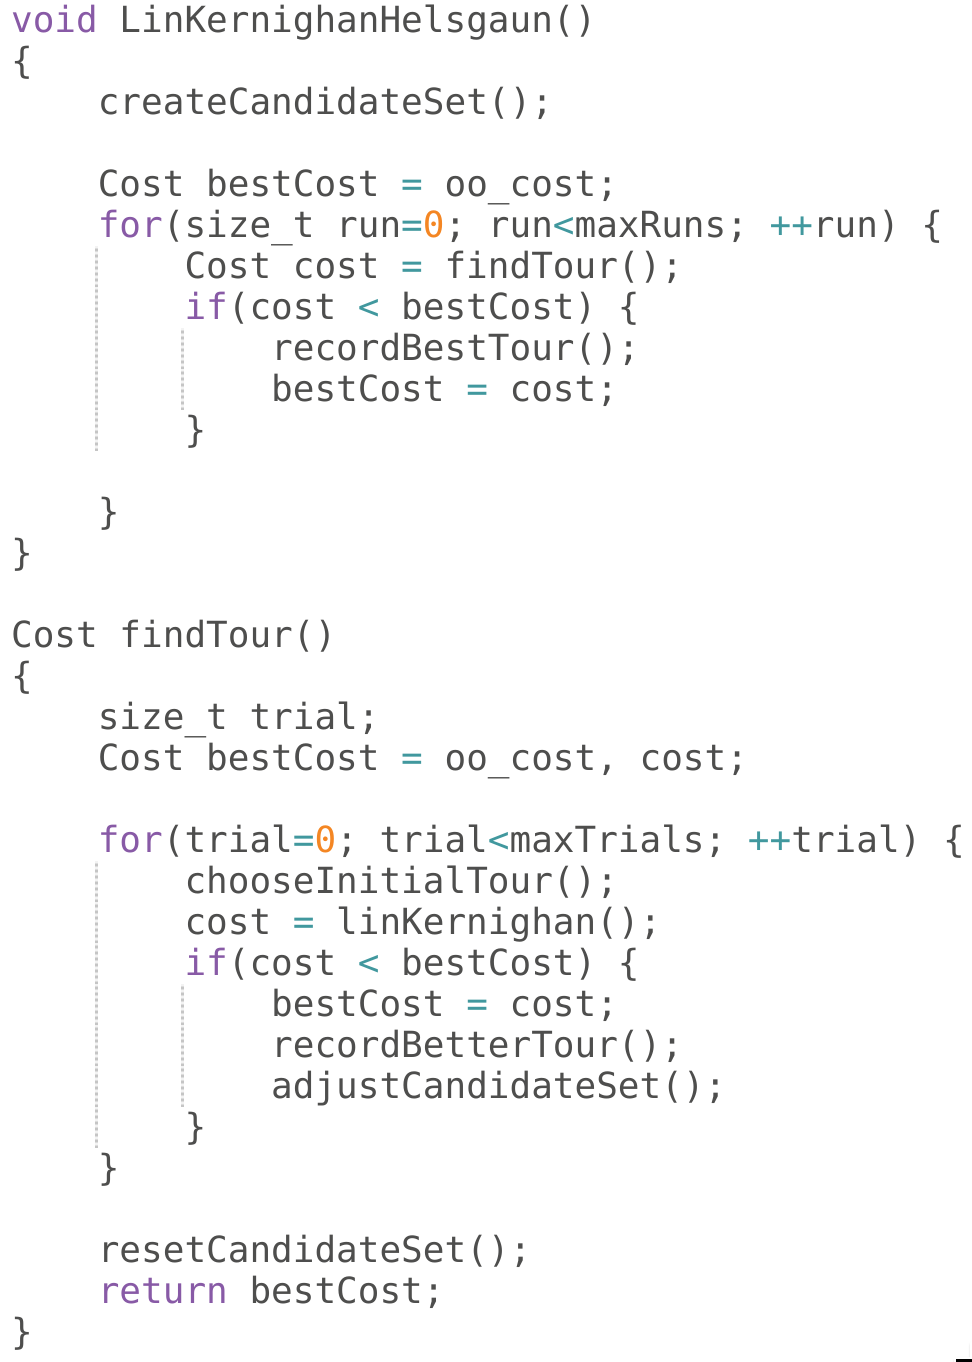
\includegraphics[width=225pt]{img/LKHProcedure.png}
    \caption{Lo ``scheletro'' della procedura.}
\end{figure}

Ogni volta che viene trovata una mossa 2-OPT o 3-OPT che porti ad un tour meno pesante, questa viene applicata.
Se, invece, non esistono tali mosse, viene applicata la mossa 3-OPT più vantaggiosa e la procedura si ripete 
cercando di ``rompere'' l'ultimo arco aggiunto dalla 3-OPT della mossa precedente; viene inoltre mantenuta 
una pila delle mosse effettuate: se si ottiene un miglioramento del tour, tale pila viene svuotata; altrimenti, 
la pila viene utilizzata per ripristinare il tour precedente (quello che potremmo definire un ``undo'').

Sono state poi analizzate le mosse 3-OPT sequenziali e si è ricavata una procedura per scomporre tali mosse in 
al più tre 2-OPT sequenziali, così da semplificare ulteriormente il codice.

\begin{figure}[H]
    \centering
    \begin{subfigure}{\linewidth}
        \centering
        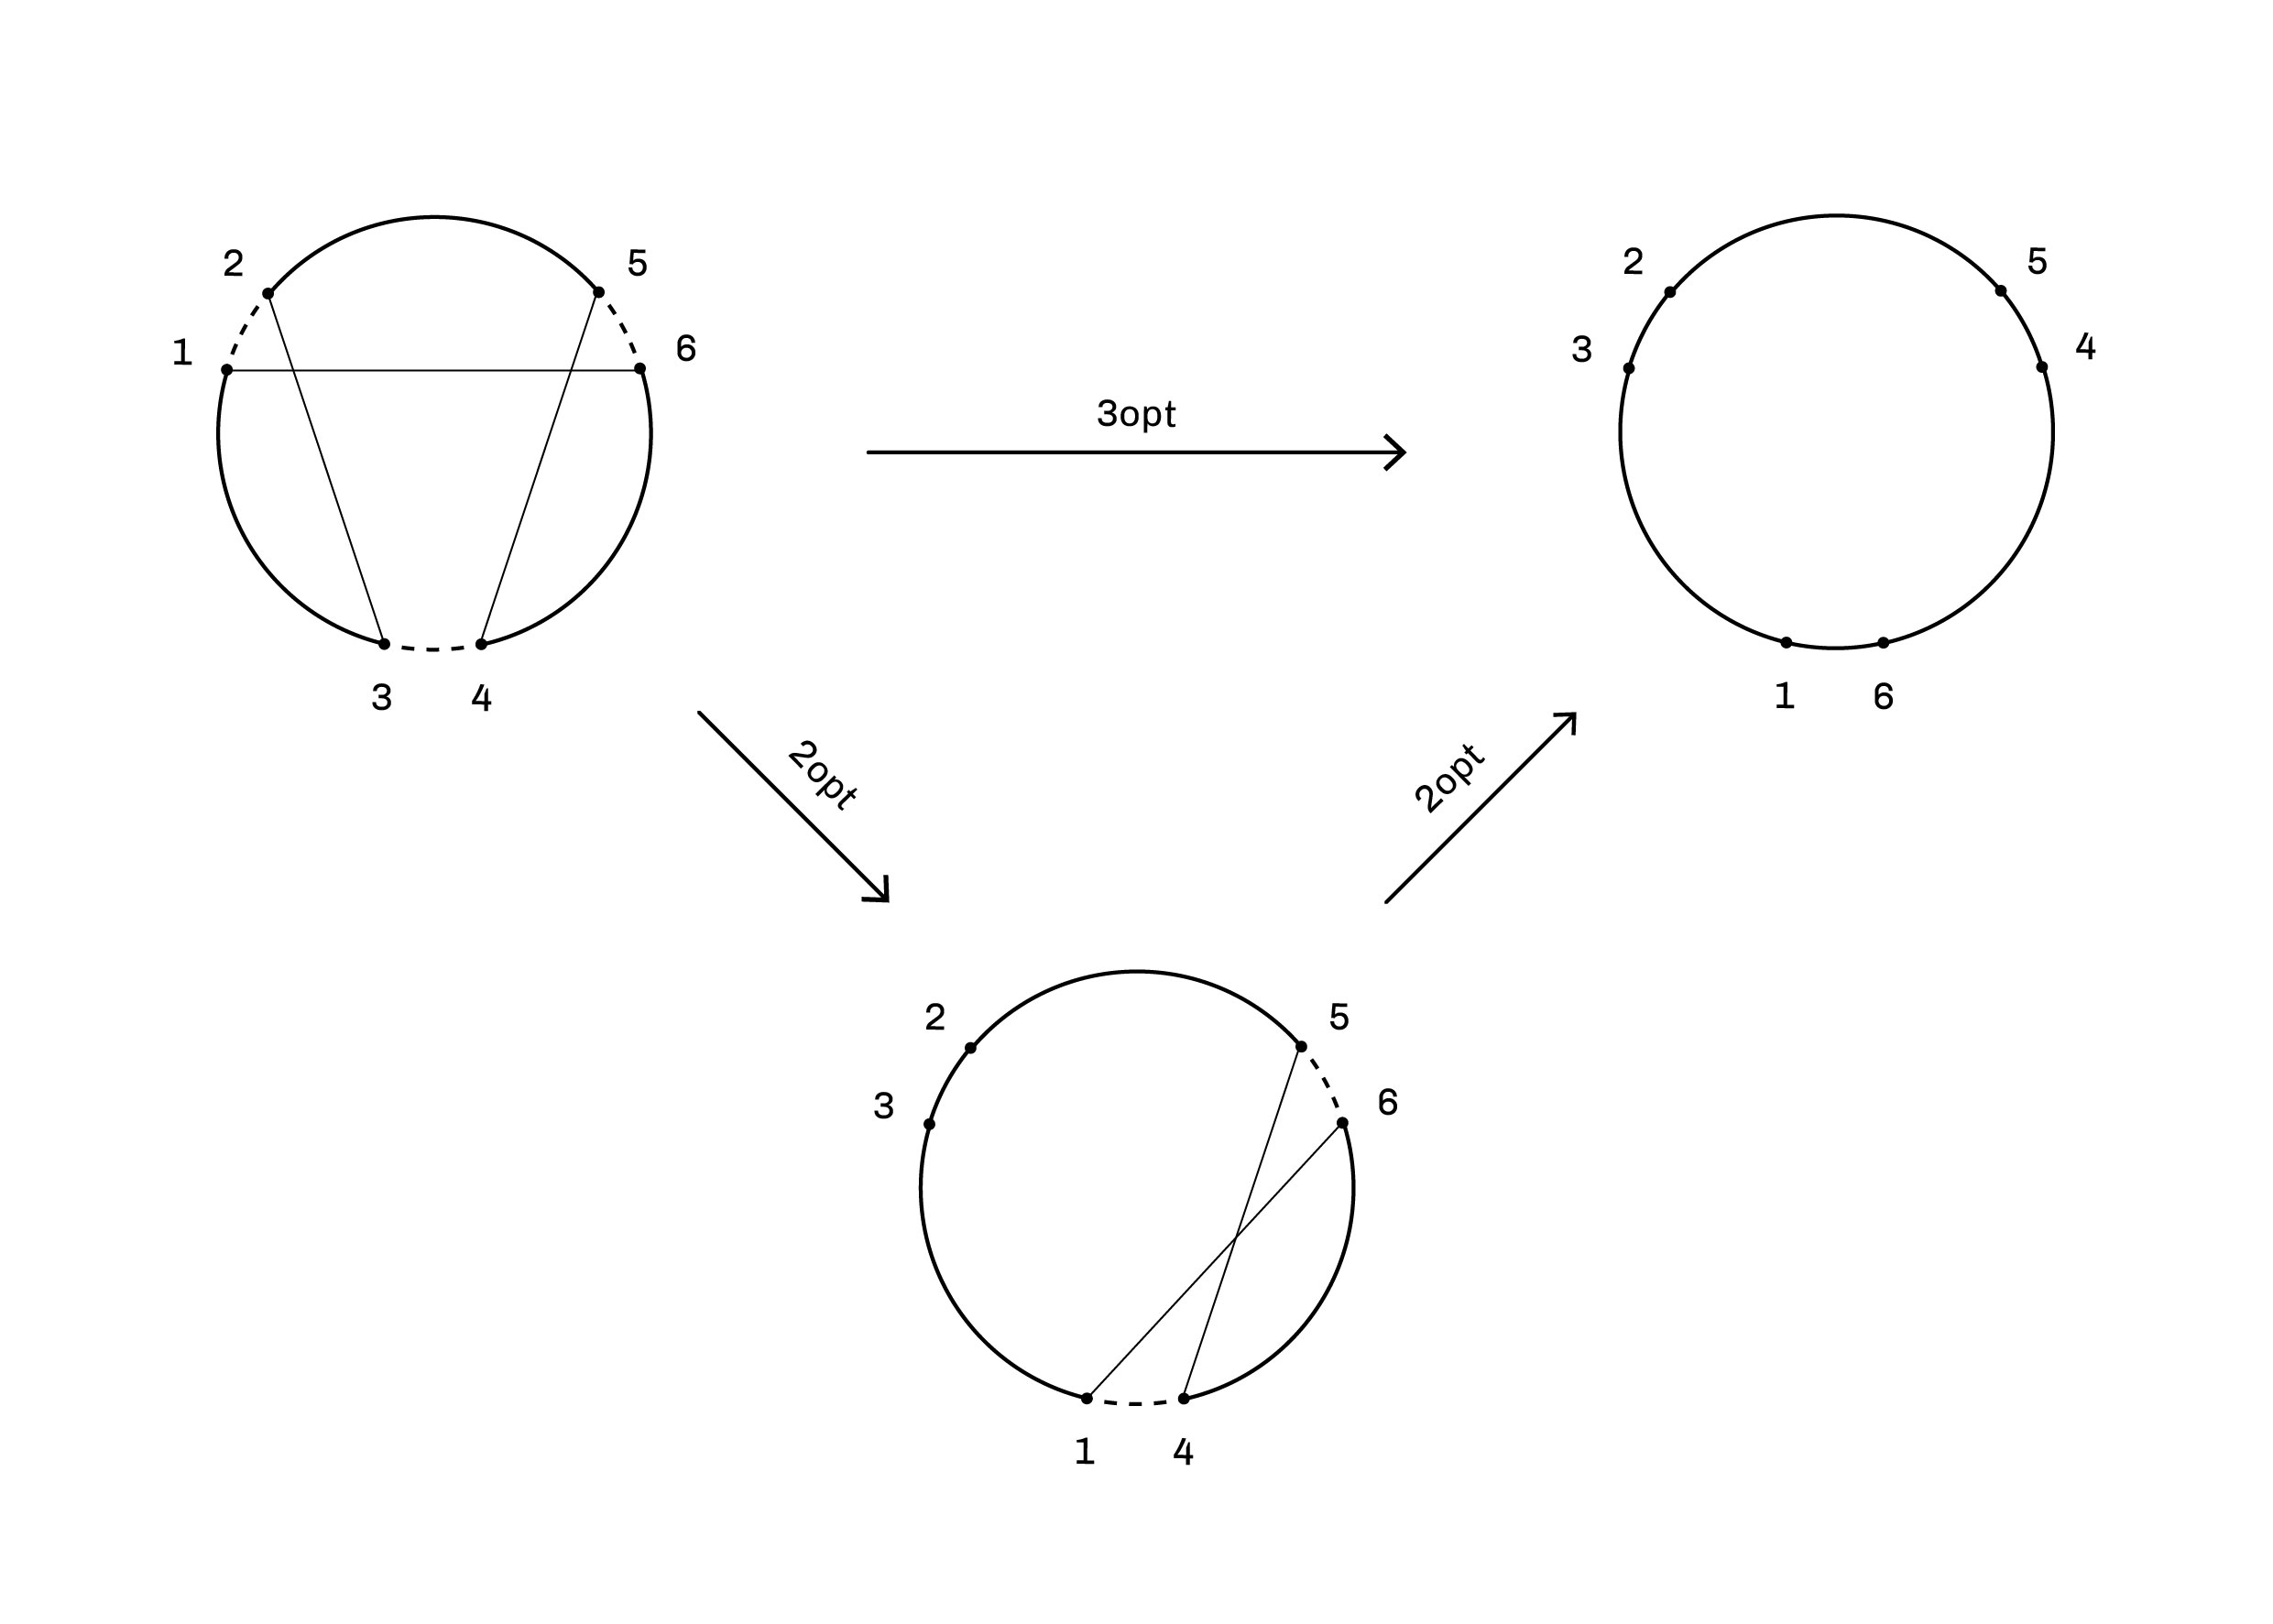
\includegraphics[width=340pt]{img/schemaH.jpg}
        \caption{}
    \end{subfigure}
    \begin{subfigure}{\linewidth}
        \centering
        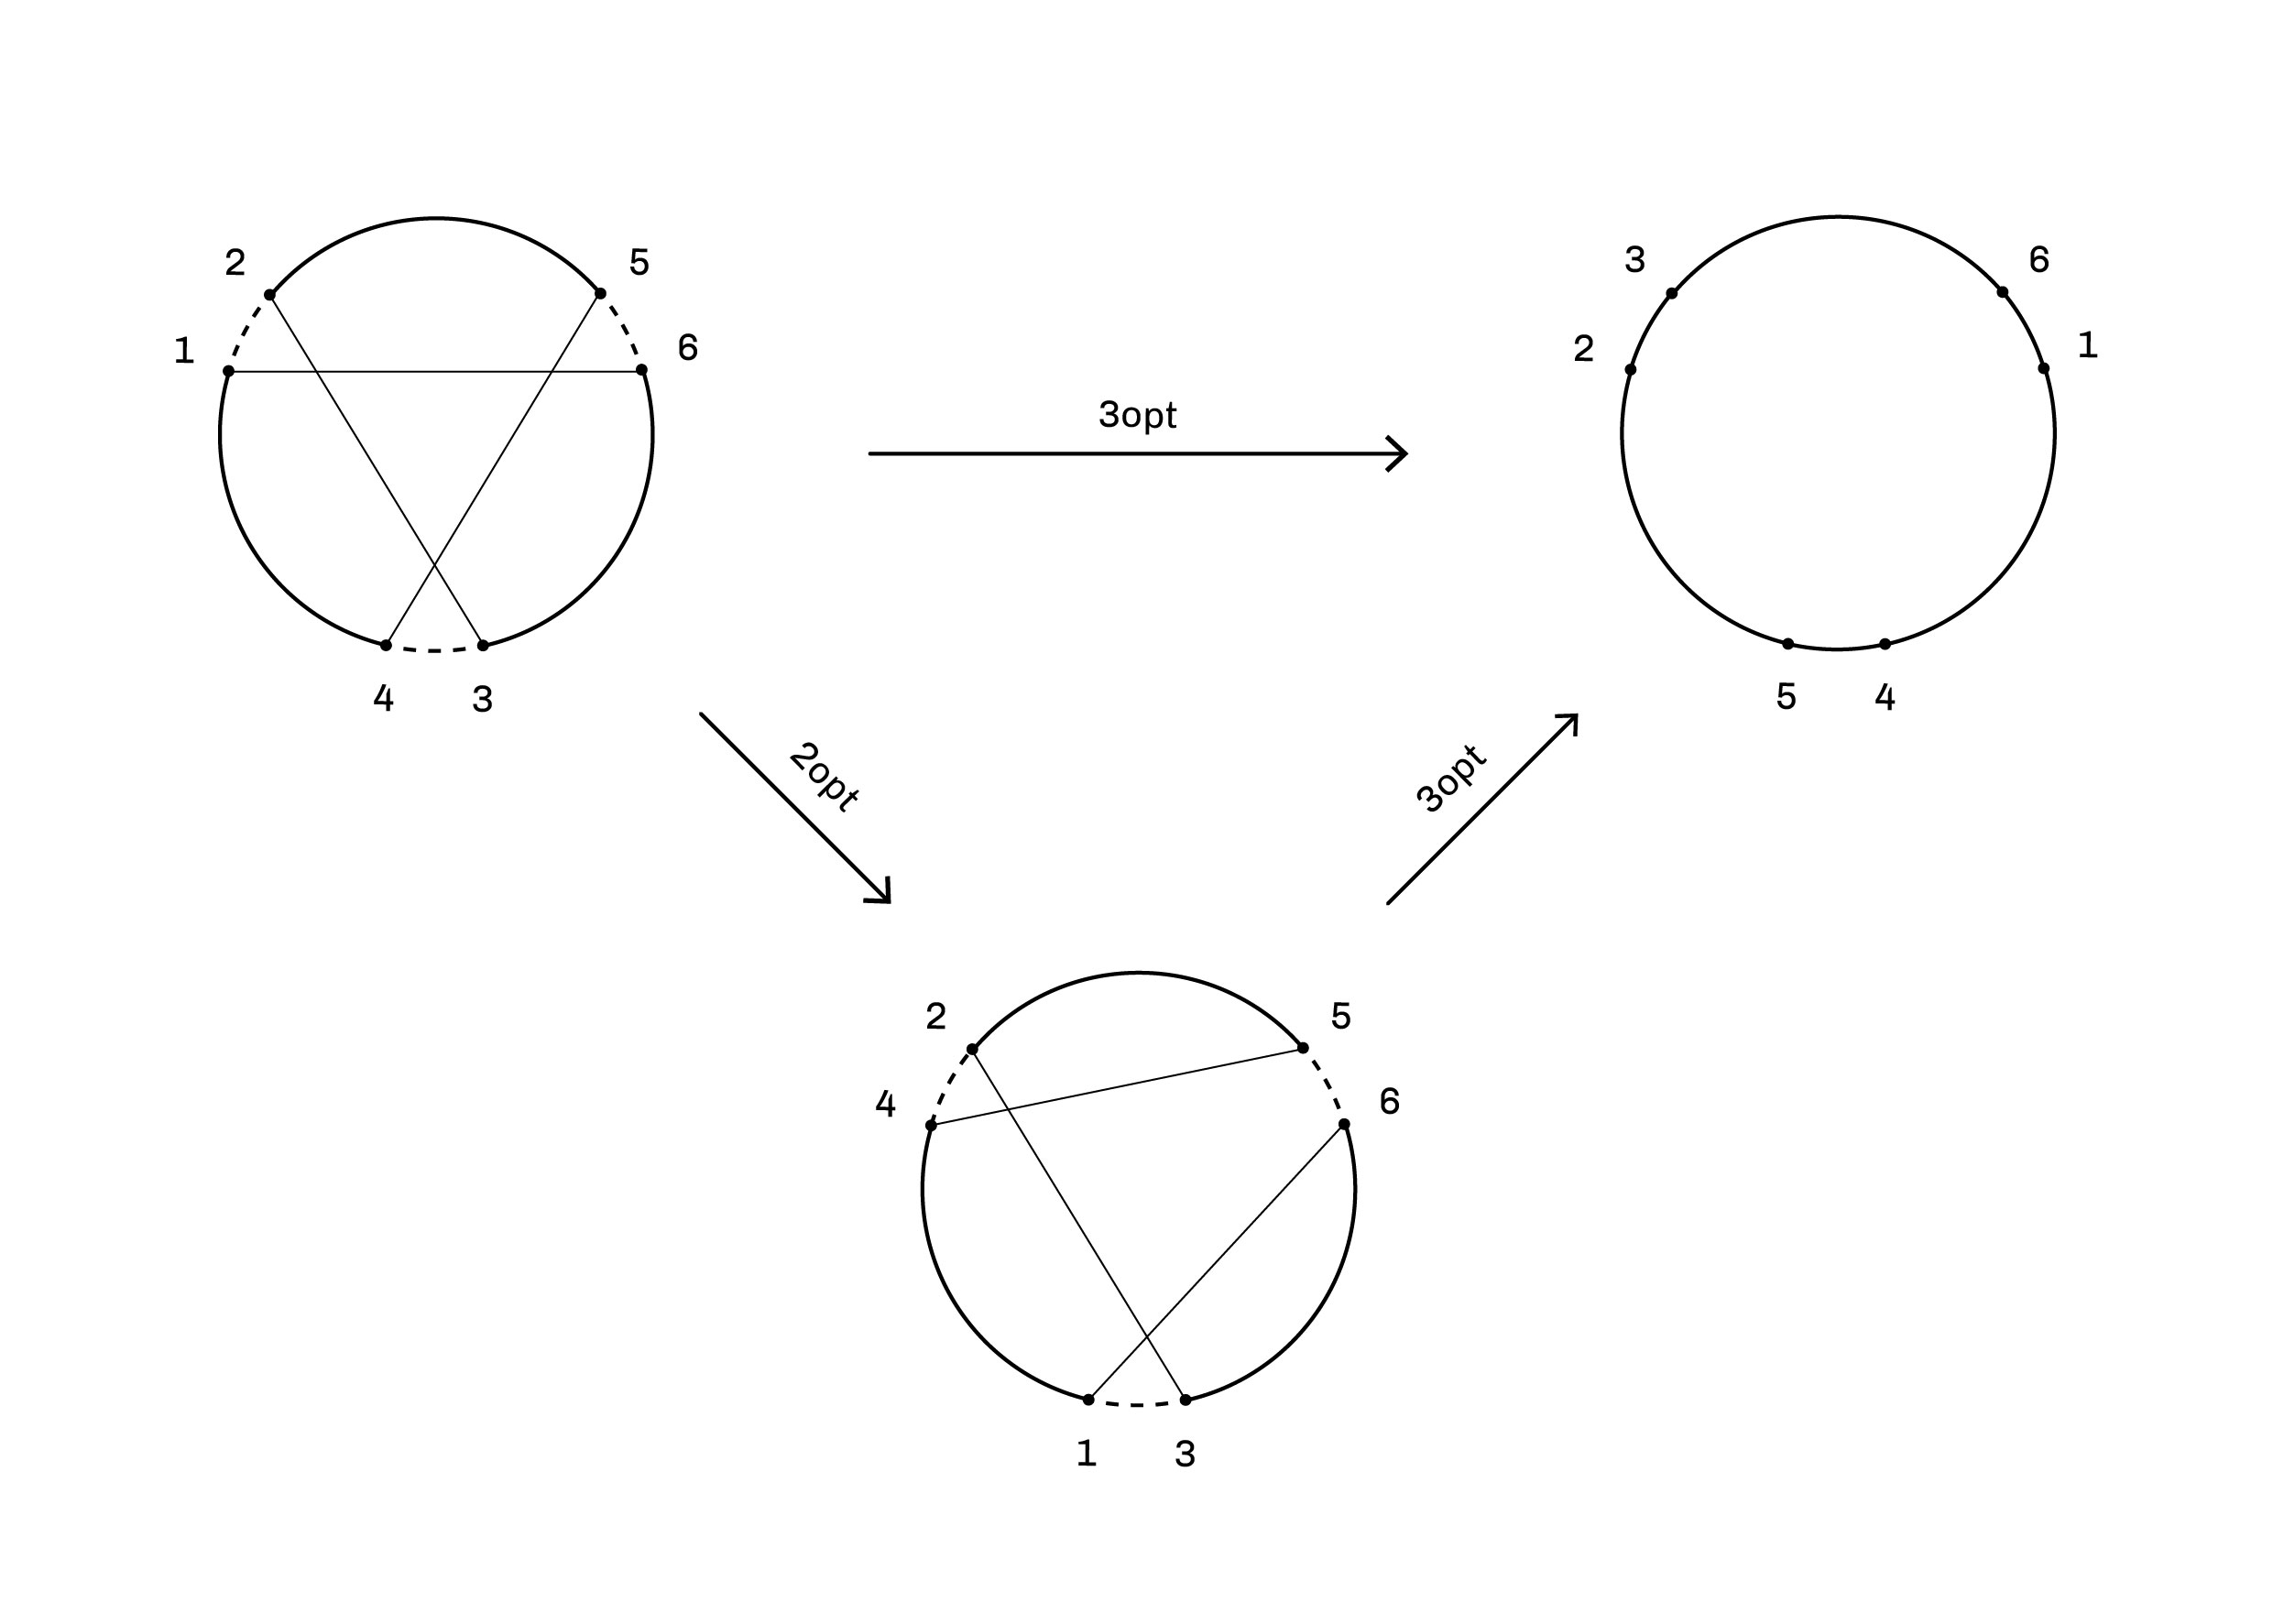
\includegraphics[width=340pt]{img/schemaXX.jpg}
        \caption{}
    \end{subfigure}
    \caption{Vengono descritte le trasformazioni che permettono di effettuare una 3-OPT come combinazione 
            di 2-OPT. Vi sono quattro tipi di 3-OPT sequenziali che emergono dall'algoritmo. Tre di 
            questi sono simmetrici per rotazione al caso (a): questo può essere simulato con due 2-OPT. 
            Notiamo poi che il quarto tipo, il caso (b), è riconducibile al caso (a) mediante un'applicazione di 2-OPT.}
\end{figure}

\section{Soggetto della misura}

Durante la fase sperimentale ci siamo focalizzati su due aspetti fondamentali di un'euristica: tempo di esecuzione 
e rapporto (empirico) di approssimazione. Sono stati utilizzati due tipi di di campione: 
\begin{itemize}
    \item Un insieme di grafi completi di $n \in \{100, 200, 300, 500, 1000, 2000, 3000, 5000\}$ nodi, con pesi 
            distribuiti uniformemente nell'intervallo $\big[1,n^2\big]\cap \mathbb{N}$.
    
    \item Un insieme di grafi presenti in \texttt{TSPLIB}; sono stati scelti \texttt{a280}, 
            \texttt{pr439}, \texttt{u1060}, \texttt{vm1748}, \texttt{pr2392}.
\end{itemize}

Inoltre, per \texttt{3-OPT} con reiterazione sono stati studiati tempo di esecuzione e qualità dell'approssimazione al variare 
di \texttt{maxExchanges}, mentre per \texttt{LKH} sono stati studiati tempo di esecuzione e qualità dell'approssimazione 
al variare di \texttt{maxCandidates}. Entrambi gli studi sono stati svolti su un campione di cinque grafi generati 
casualmente di $n=1000$ nodi.

La qualità dell'approssimazione è l'errore relativo del costo del tour trovato dall'euristica rispetto al costo ottimo,
$$\epsilon = \frac{C_{eur}-C_{opt}}{C_{opt}}$$

Per le istanze scelte di \texttt{TSPLIB} l'ottimo è noto; per i grafi generati casualmente si è cercato di approssimare 
l'ottimo con la bound di Held-Karp calcolata attraverso \texttt{ascent}. Sfortunatamente, la differenza percentuale tra 
le bound approssimate e i costi dei tour superavano, in alcuni casi, i $5000$ punti: l'ipotesi è che la distribuzione 
uniforme dei costi degli archi abbia sensibilmente abbassato la bound di Held-Karp rispetto al tour ottimo. In mancanza 
di evidenze sperimentali che ci permettessero di sfruttare efficacemente il valore calcolato da \texttt{ascent} si è 
deciso di non assegnare un errore ai costi dei tour nei grafi casuali.

\section{Modalità di misurazione del tempo di esecuzione}

La macchina su cui sono stati svolti i test è un Dell XPS-13 9370 con cpu Intel Core i5-82500U, 4 core (8 thread) da 
1.60GHz (3.40GHz in Turbo Boost) e 8GB di memoria Ram.

Per evitare di incorrere in risultati non affidabili la misurazione del tempo di esecuzione è stata svolta 
seguendo la procedura descritta in \cite{Poli}. È stato definito un'intervallo di confidenza all'$(1-\alpha)$ 
per $\alpha=0.05$ e, per ogni dimensione $n$, è stato generato un campione di cinque grafi di $n$ nodi: per quanto 
riguarda i grafi di \texttt{TSPLIB} tale campione è stato costruito con cinque copie dello stesso grafo.

\section{Randomness}

La casualità è uno strumento fondamentale nell'Informatica: essa permette di ottenere algoritmi più efficienti, 
strutture dati più robuste e simulazioni più realistiche. Ognuna delle euristiche descritte utilizza, in misura 
diversa, la \textit{randomness}. Non solo, anche la procedura di misurazione descritta precedentemente utilizza 
la randomness per la generazione dei campioni. È quindi necessario un algoritmo che approssimi 
sufficientemente bene la casualità: a differenza del linguaggio \texttt{C} e altri, il \texttt{C++} mette a 
disposizione la libreria \texttt{<random>} per gestire distribuzioni e generatori di numeri (pseudo)casuali. 
Tra i generatori lineari congruenziali è presente un'implementazione del prng Park-Miller (che viene 
utilizzato anche in \cite{Poli}). È stato quindi scelto tale generatore per effettuare ogni operazione che 
coinvolgesse la randomness.

\section{Risultati e confronti}

\subsection{Tabelle dei risultati}

Vengono di seguito presentati i risultati degli esperimenti effettuati. I tempi sono espressi in 
secondi, ``Errore (\%)'' è $\epsilon\cdot{}100$, ``Diff T (\%)'' e ``Diff C (\%)'' sono le differenze 
percentuali rispetto al valore di riferimenti: nel caso di \texttt{RL3O} è di $10$ scambi, nel caso di 
\texttt{LKH} è di $30$ candidati. In questa sottosezione ci limitiamo a fornire le tabelle dei dati; 
questi verranno confrontati e commentati nella successiva.
\ \\
\ \\
\ \\

\begin{figure}[H]
    \centering
    \begin{subfigure}{\linewidth}
        \centering
        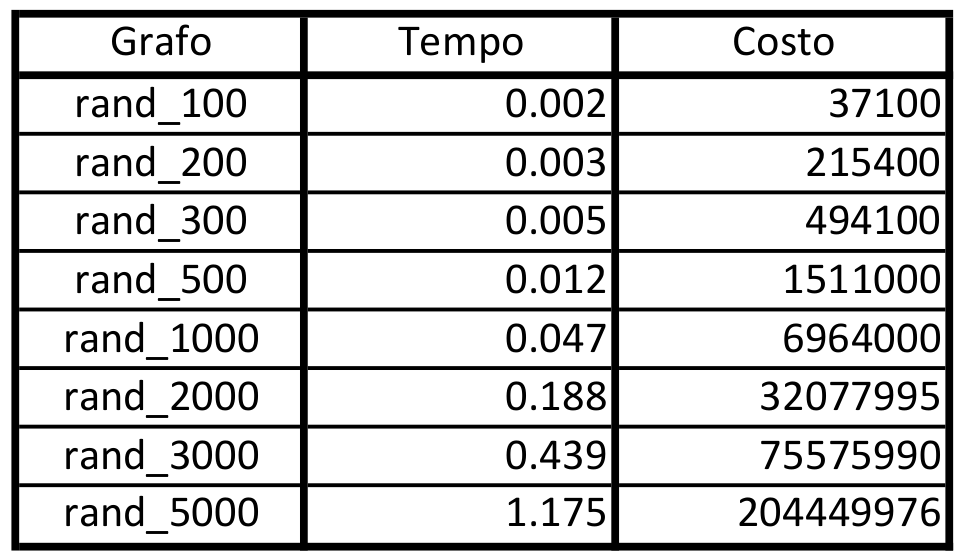
\includegraphics[width=200pt]{img/NNrandom.png}
        \caption*{Su grafi generati casualmente.}
    \end{subfigure}
    \ \\
    \ \\
    \ \\
    \ \\
    \begin{subfigure}{\linewidth}
        \centering
        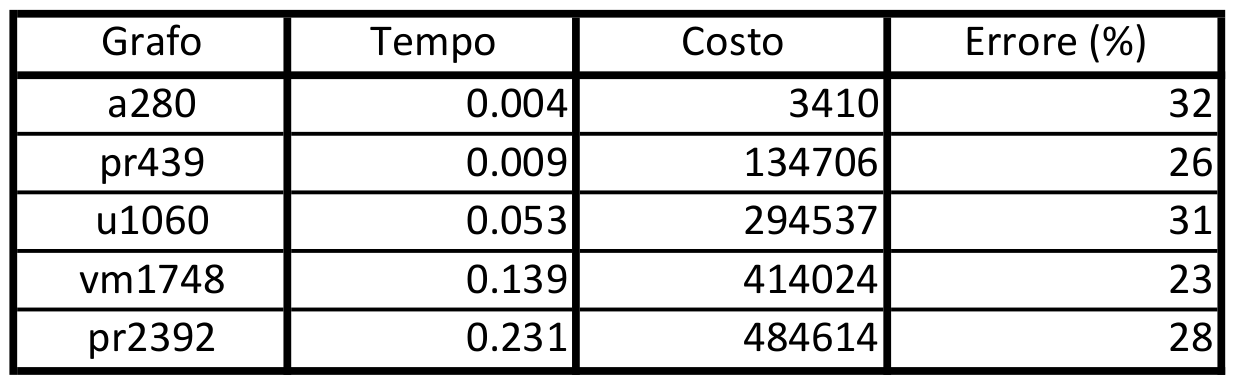
\includegraphics[width=300pt]{img/NNtsplib.png}
        \caption*{Su grafi di \texttt{TSPLIB}.}
    \end{subfigure}
    \caption{Risultati \texttt{NN}.}
\end{figure}
\ \\
\ \\

\begin{figure}[H]
    \centering
    \begin{subfigure}{\linewidth}
        \centering
        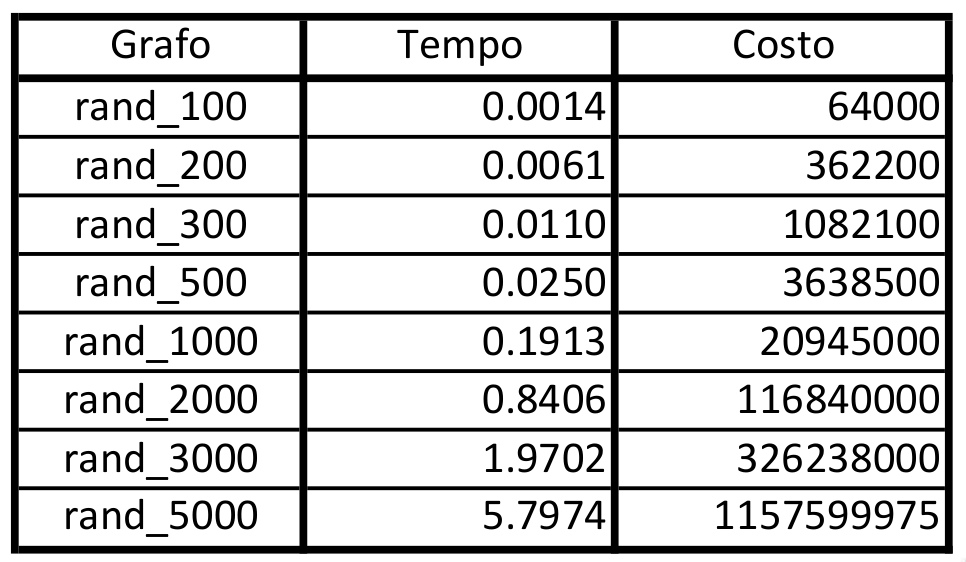
\includegraphics[width=200pt]{img/NIrandom.png}
        \caption*{Su grafi generati casualmente.}
    \end{subfigure}
    \ \\
    \ \\
    \ \\
    \ \\
    \begin{subfigure}{\linewidth}
        \centering
        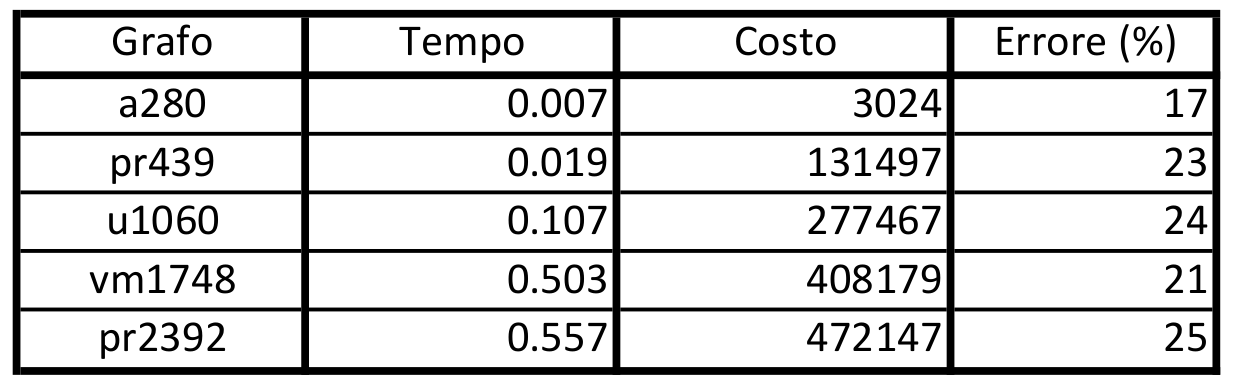
\includegraphics[width=300pt]{img/NItsplib.png}
        \caption*{Su grafi di \texttt{TSPLIB}.}
    \end{subfigure}
    \caption{Risultati \texttt{NI}.}
\end{figure}
\ \\
\ \\

\begin{figure}[H]
    \centering
    \begin{subfigure}{\linewidth}
        \centering
        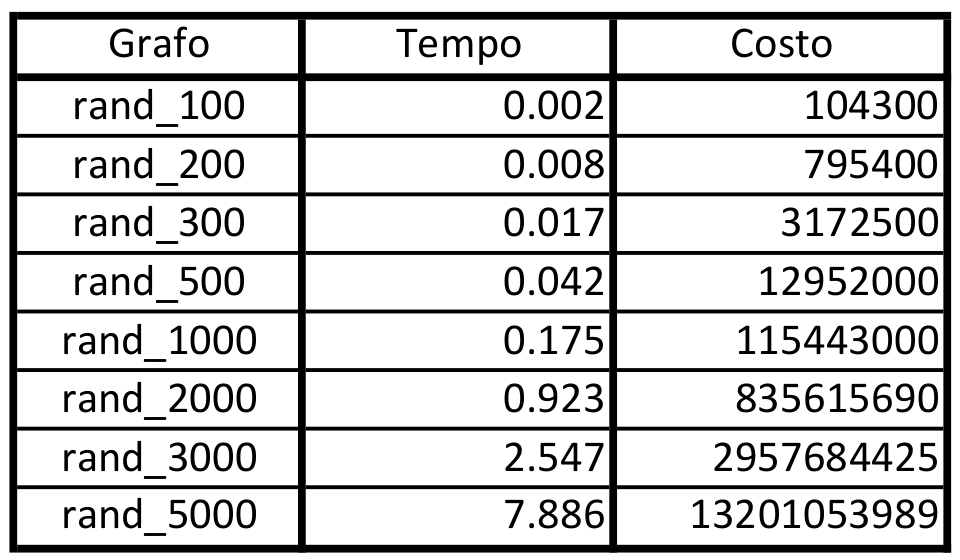
\includegraphics[width=200pt]{img/CHRrandom.png}
        \caption*{Su grafi generati casualmente.}
    \end{subfigure}
    \ \\
    \ \\
    \ \\
    \ \\
    \begin{subfigure}{\linewidth}
        \centering
        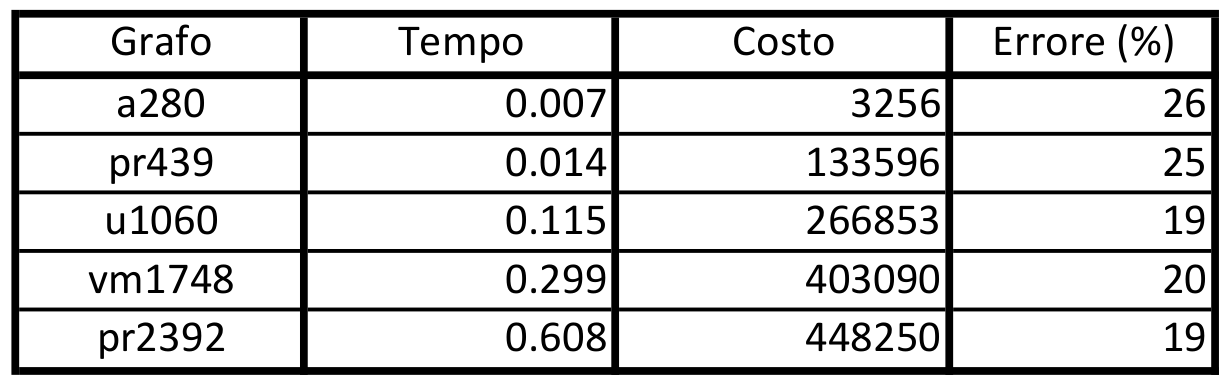
\includegraphics[width=300pt]{img/CHRtsplib.png}
        \caption*{Su grafi di \texttt{TSPLIB}.}
    \end{subfigure}
    \caption{Risultati \texttt{CHR}.}
\end{figure}
\ \\
\ \\

\begin{figure}[H]
    \centering
    \begin{subfigure}{\linewidth}
        \centering
        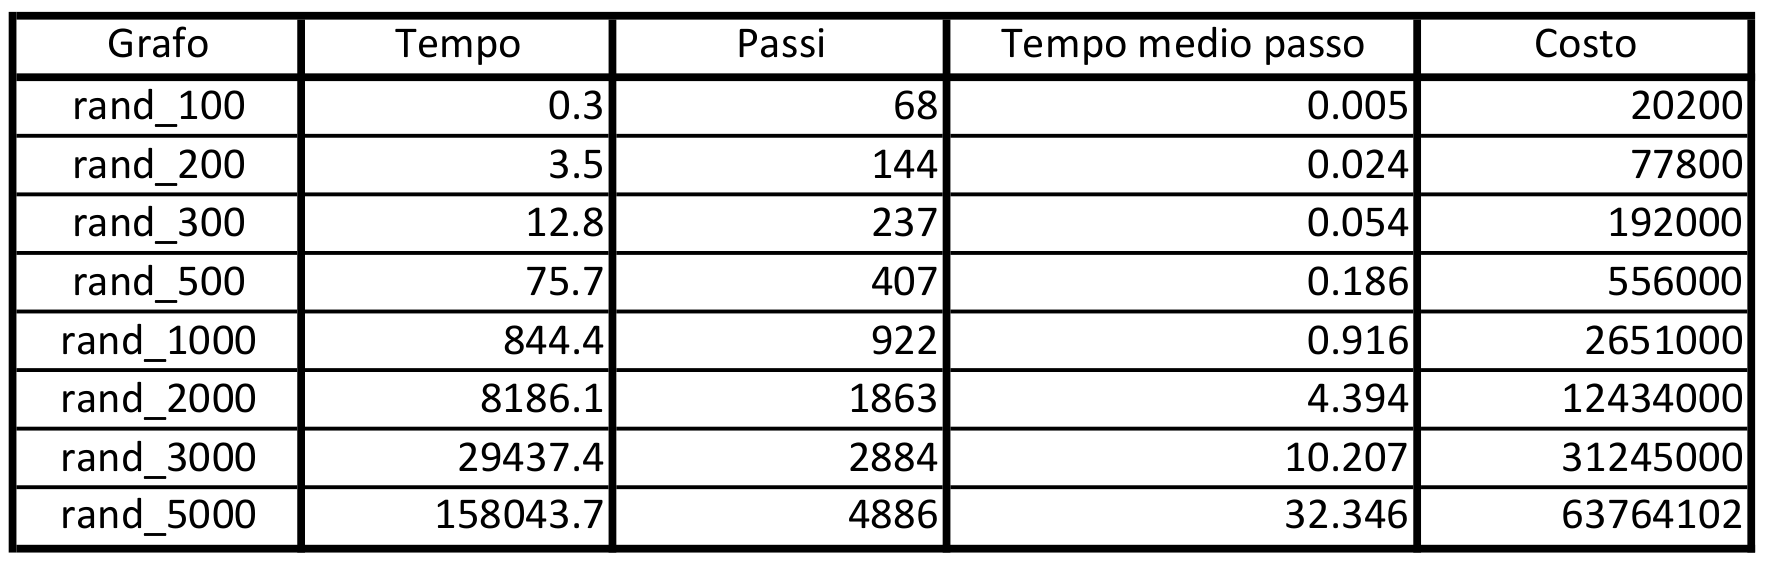
\includegraphics[width=400pt]{img/L3ORrandom.png}
        \caption*{Su grafi generati casualmente.}
    \end{subfigure}
    \ \\
    \ \\
    \ \\
    \ \\
    \begin{subfigure}{\linewidth}
        \centering
        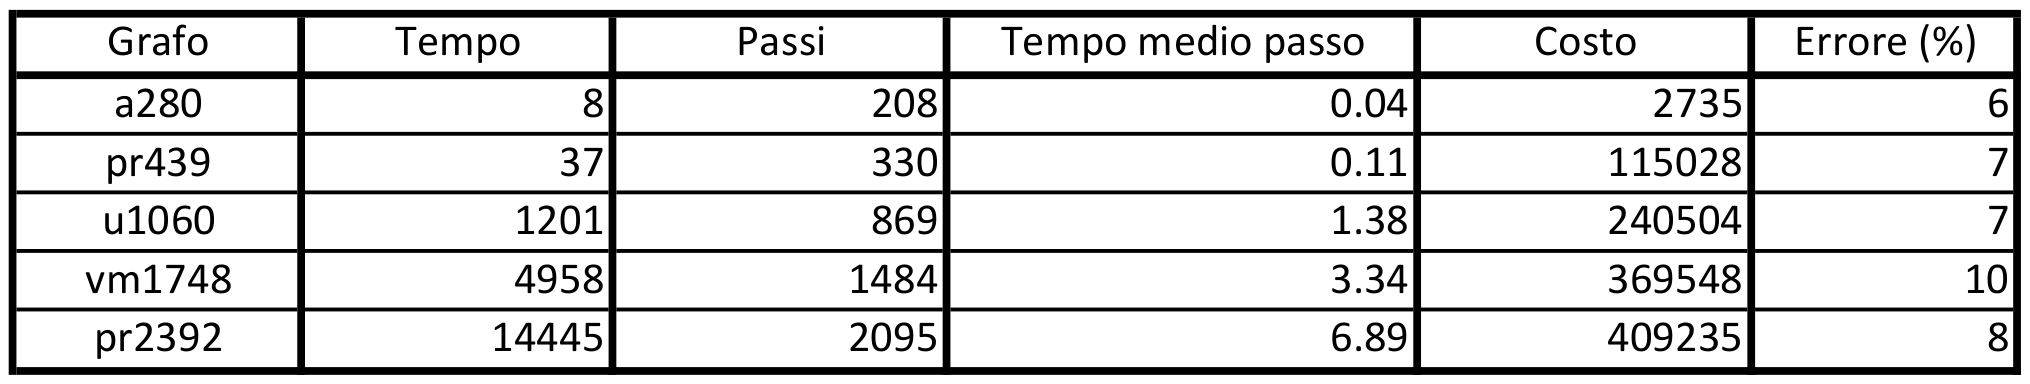
\includegraphics[width=400pt]{img/L3ORtsplib.png}
        \caption*{Su grafi di \texttt{TSPLIB}.}
    \end{subfigure}
    \caption{Risultati \texttt{L3OR}.}
\end{figure}
\ \\

\begin{figure}[H]
    \centering
    \begin{subfigure}{\linewidth}
        \centering
        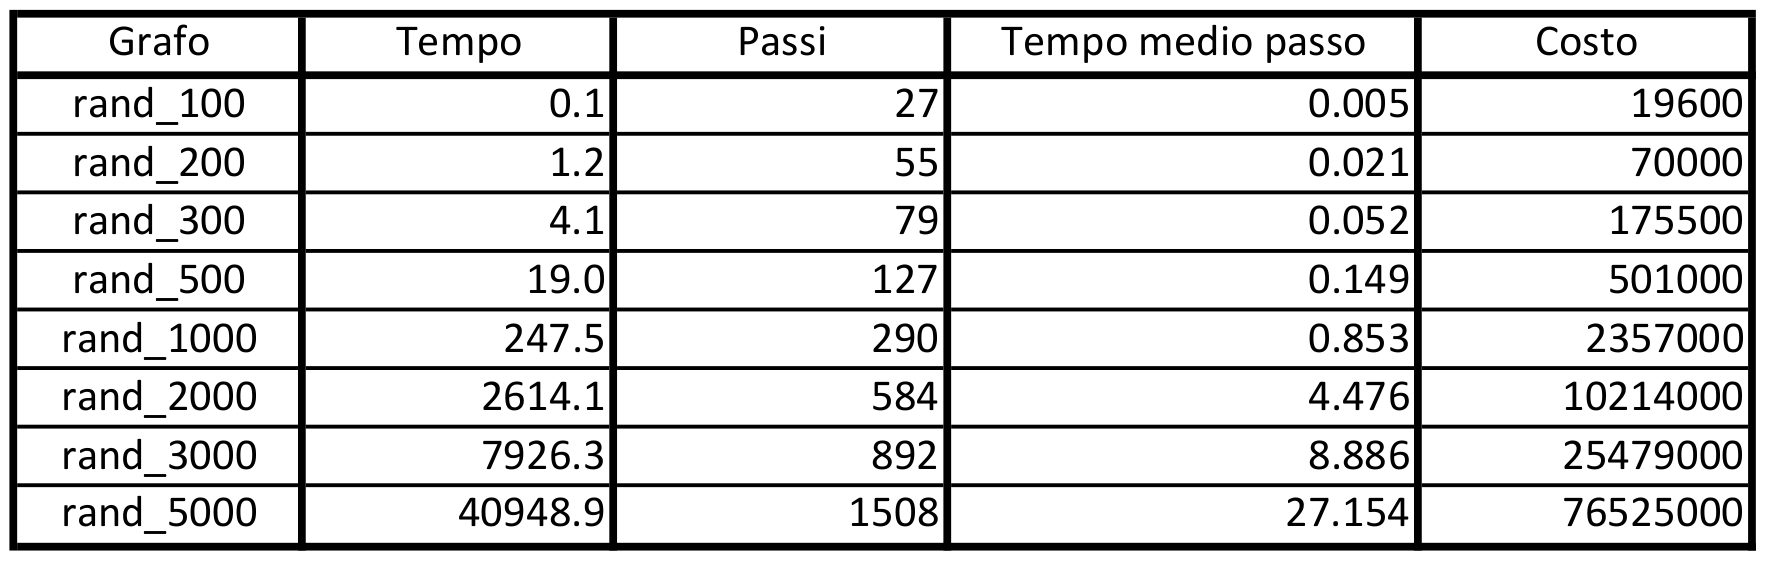
\includegraphics[width=400pt]{img/L3OCrandom.png}
        \caption*{Su grafi generati casualmente.}
    \end{subfigure}
    \ \\
    \ \\
    \ \\
    \ \\
    \begin{subfigure}{\linewidth}
        \centering
        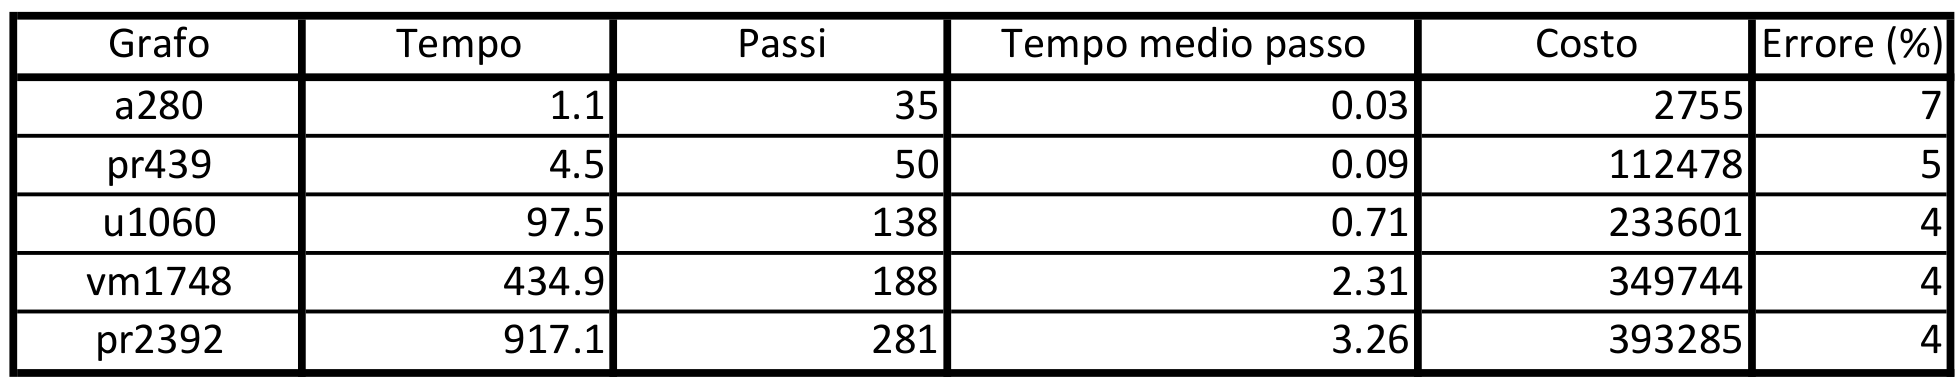
\includegraphics[width=400pt]{img/L3OCtsplib.png}
        \caption*{Su grafi di \texttt{TSPLIB}.}
    \end{subfigure}
    \caption{Risultati \texttt{L3OC}.}
\end{figure}
\ \\
\ \\

\begin{figure}[H]
    \centering
    \begin{subfigure}{\linewidth}
        \centering
        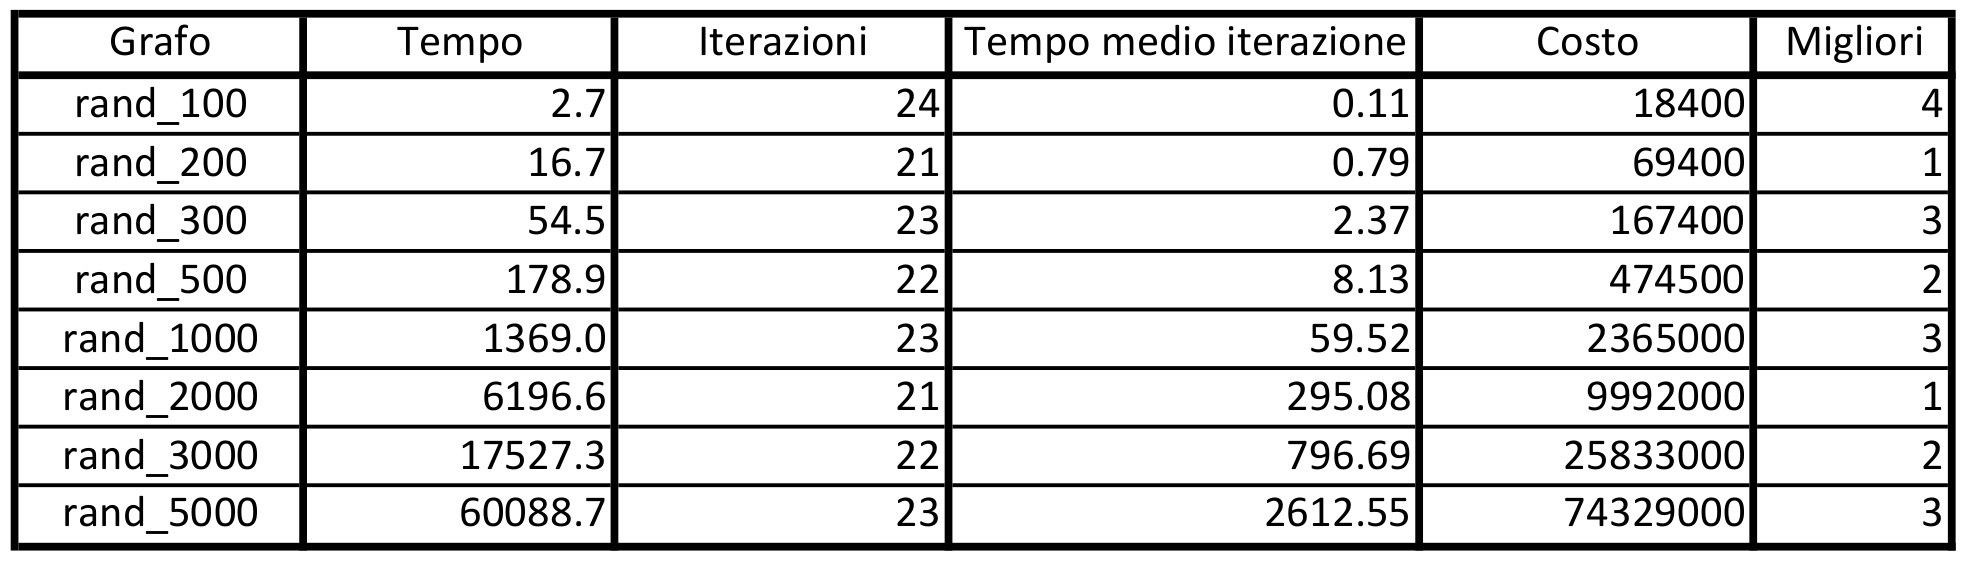
\includegraphics[width=400pt]{img/RL3Orandom.png}
        \caption*{Su grafi generati casualmente.}
    \end{subfigure}
    \ \\
    \ \\
    \ \\
    \ \\
    \begin{subfigure}{\linewidth}
        \centering
        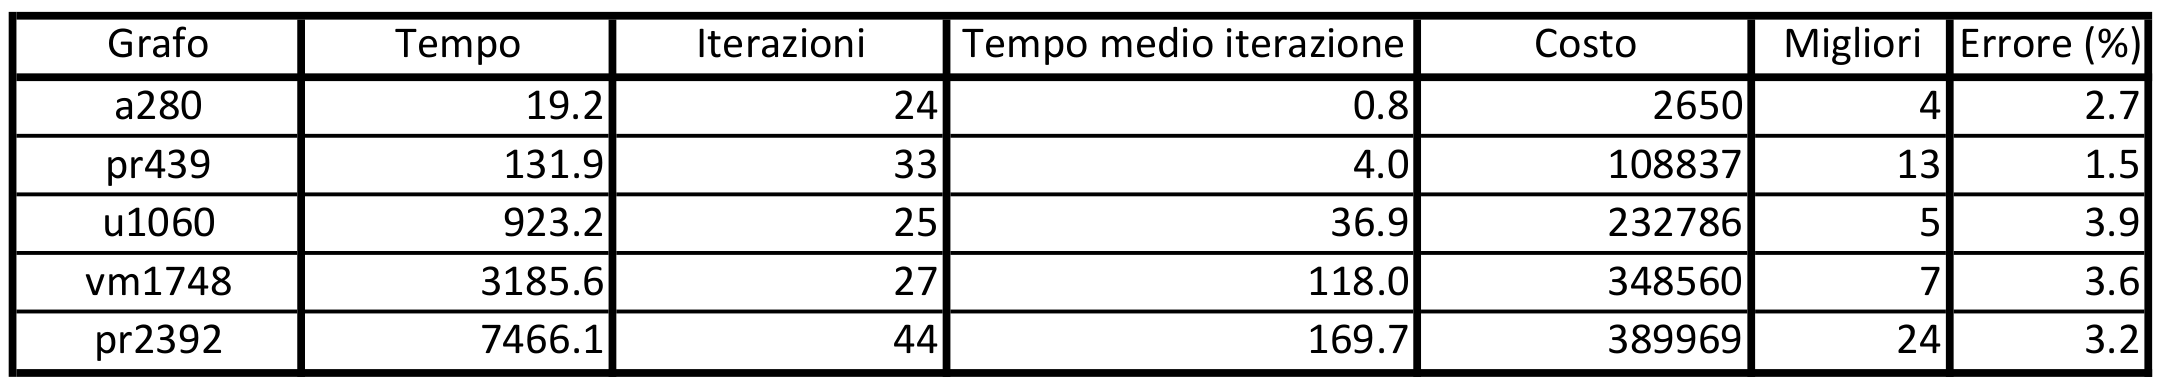
\includegraphics[width=400pt]{img/RL3Otsplib.png}
        \caption*{Su grafi di \texttt{TSPLIB}.}
    \end{subfigure}
    \ \\
    \ \\
    \ \\
    \ \\
    \begin{subfigure}{\linewidth}
        \centering
        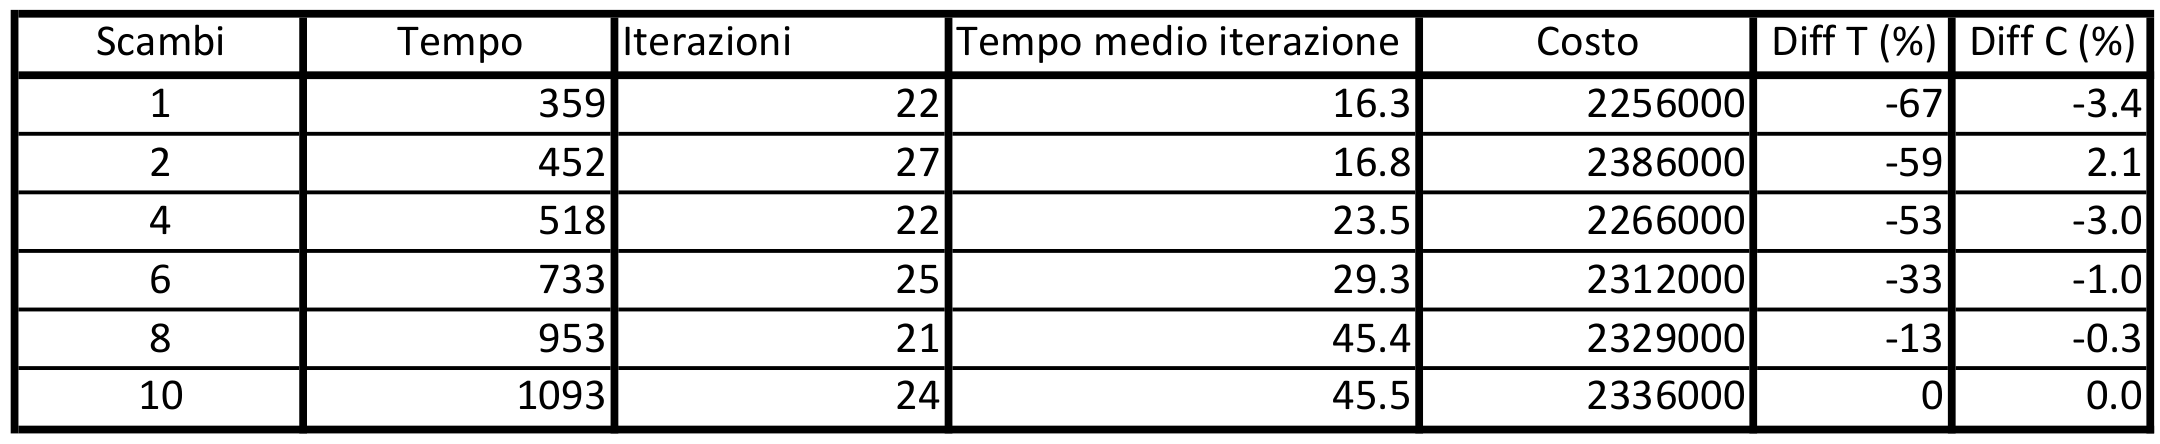
\includegraphics[width=400pt]{img/RL3Oscambi.png}
        \caption*{Su un campione di grafi causali di $n=1000$ nodi, al variare di \texttt{maxExchanges}.}
    \end{subfigure}
    \caption{Risultati \texttt{RL3O}.}
\end{figure}
\ \\
\ \\

\begin{figure}[H]
    \centering
    \begin{subfigure}{\linewidth}
        \centering
        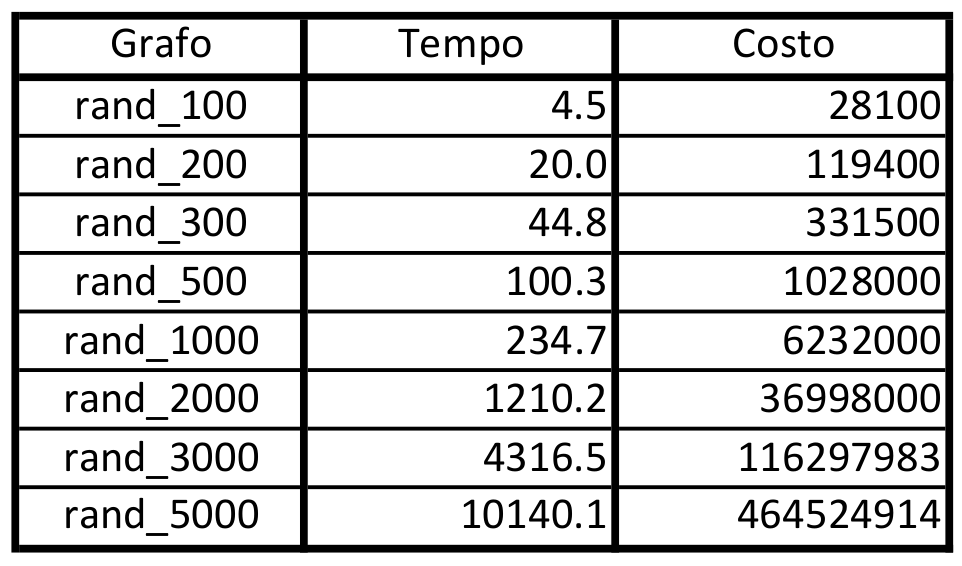
\includegraphics[width=200pt]{img/LKHrandom.png}
        \caption*{Su grafi generati casualmente.}
    \end{subfigure}
    \ \\
    \ \\
    \ \\
    \ \\
    \begin{subfigure}{\linewidth}
        \centering
        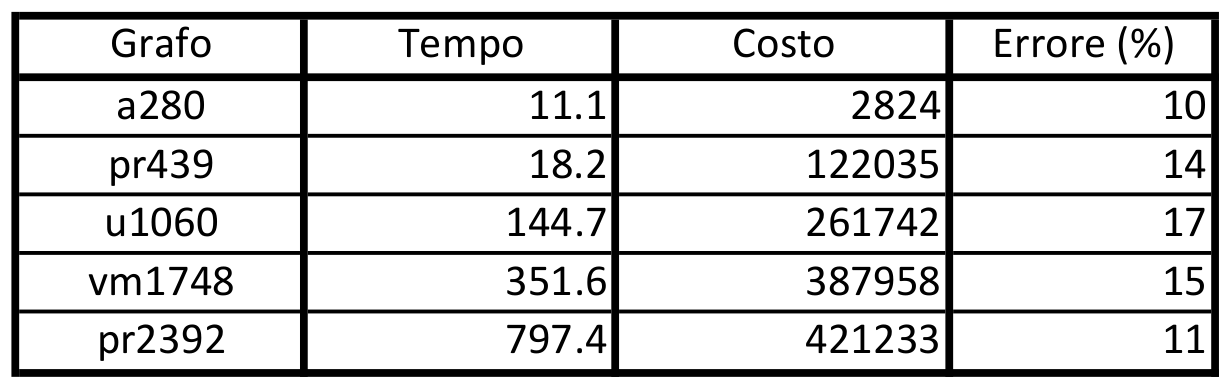
\includegraphics[width=300pt]{img/LKHtsplib.png}
        \caption*{Su grafi di \texttt{TSPLIB}.}
    \end{subfigure}
    \ \\
    \ \\
    \ \\
    \ \\
    \begin{subfigure}{\linewidth}
        \centering
        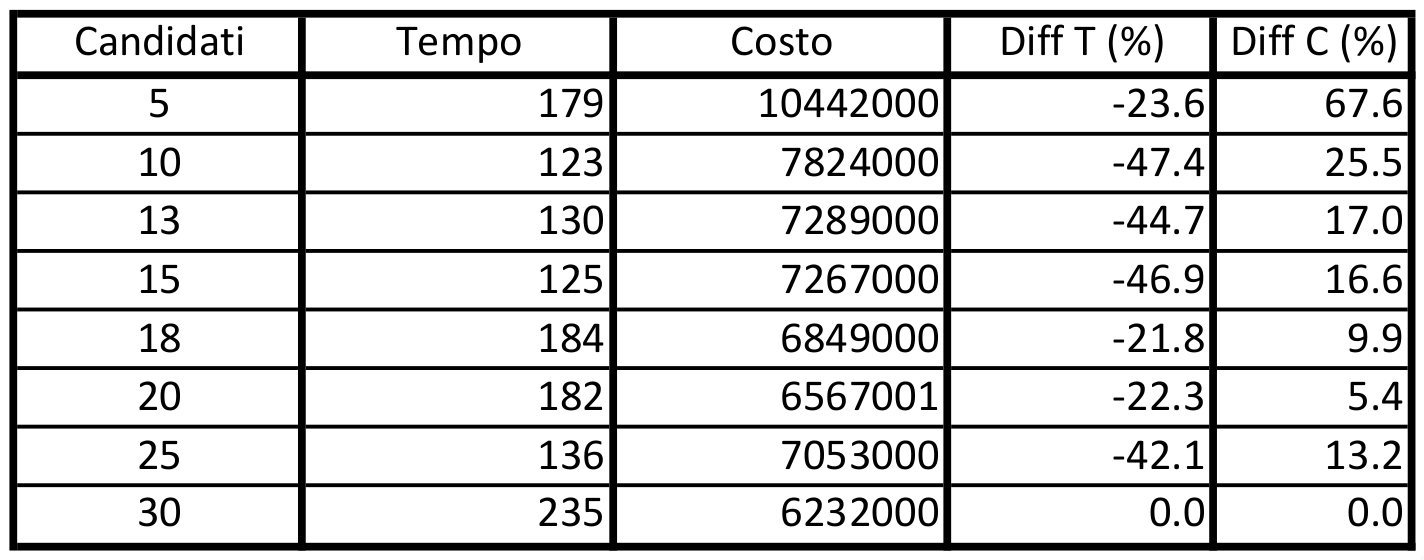
\includegraphics[width=300pt]{img/LKHcandidati.png}
        \caption*{Su un campione di grafi causali di $n=1000$ nodi, al variare di \texttt{maxCandidates}.}
    \end{subfigure}
    \caption{Risultati \texttt{LKH}.}
\end{figure}

\newpage
\subsection{Tabelle e grafici dei confronti}

Vengono ora confrontati e commentati i risultati ottenuti: tempi e costi tra diverse euristiche, confronto 
nel numero di scambi in \texttt{RL3O} e confronto nel numero di candidati in \texttt{LKH}.

\begin{figure}[H]
    \centering
    \begin{subfigure}{\linewidth}
        \centering
        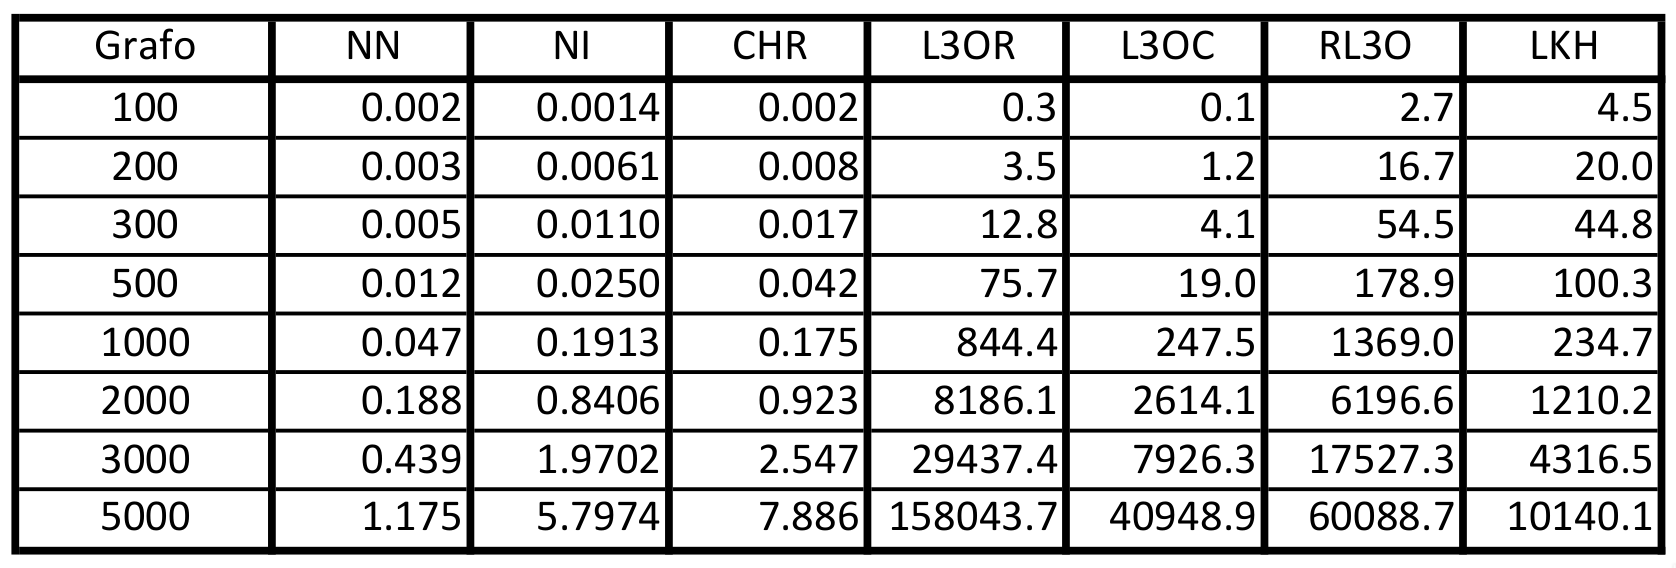
\includegraphics[width=320pt]{img/ConfrontoTempiRandom.png}
        \caption*{Su grafi generati casualmente.}
    \end{subfigure}
    \ \\
    \ \\
    \ \\
    \begin{subfigure}{\linewidth}
        \centering
        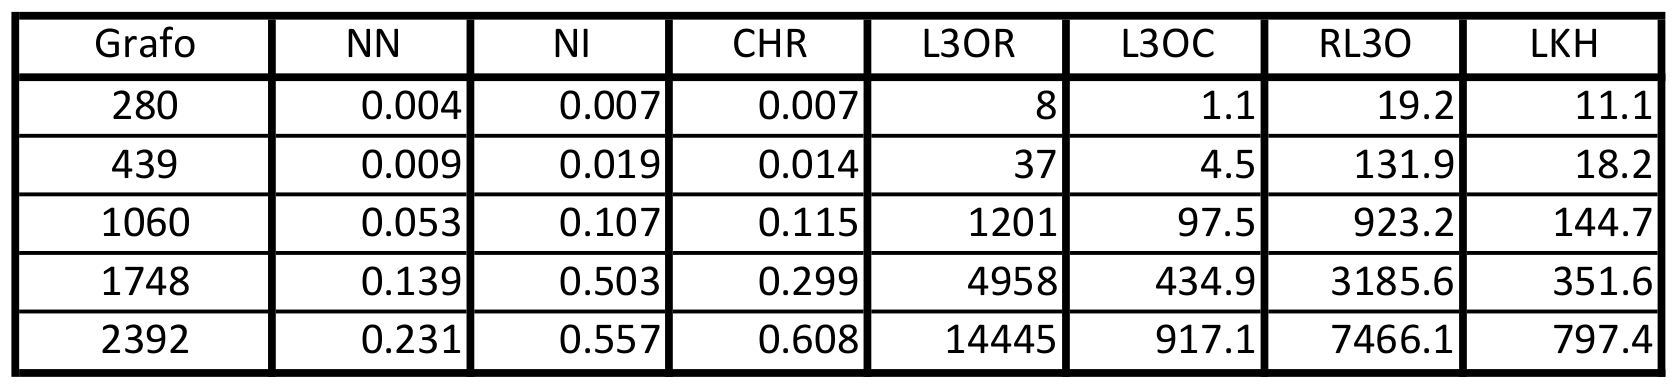
\includegraphics[width=320pt]{img/ConfrontoTempiTsplib.png}
        \caption*{Su grafi di \texttt{TSPLIB}.}
    \end{subfigure}
    \ \\
    \ \\
    \ \\
    \begin{subfigure}{\linewidth}
        \centering
        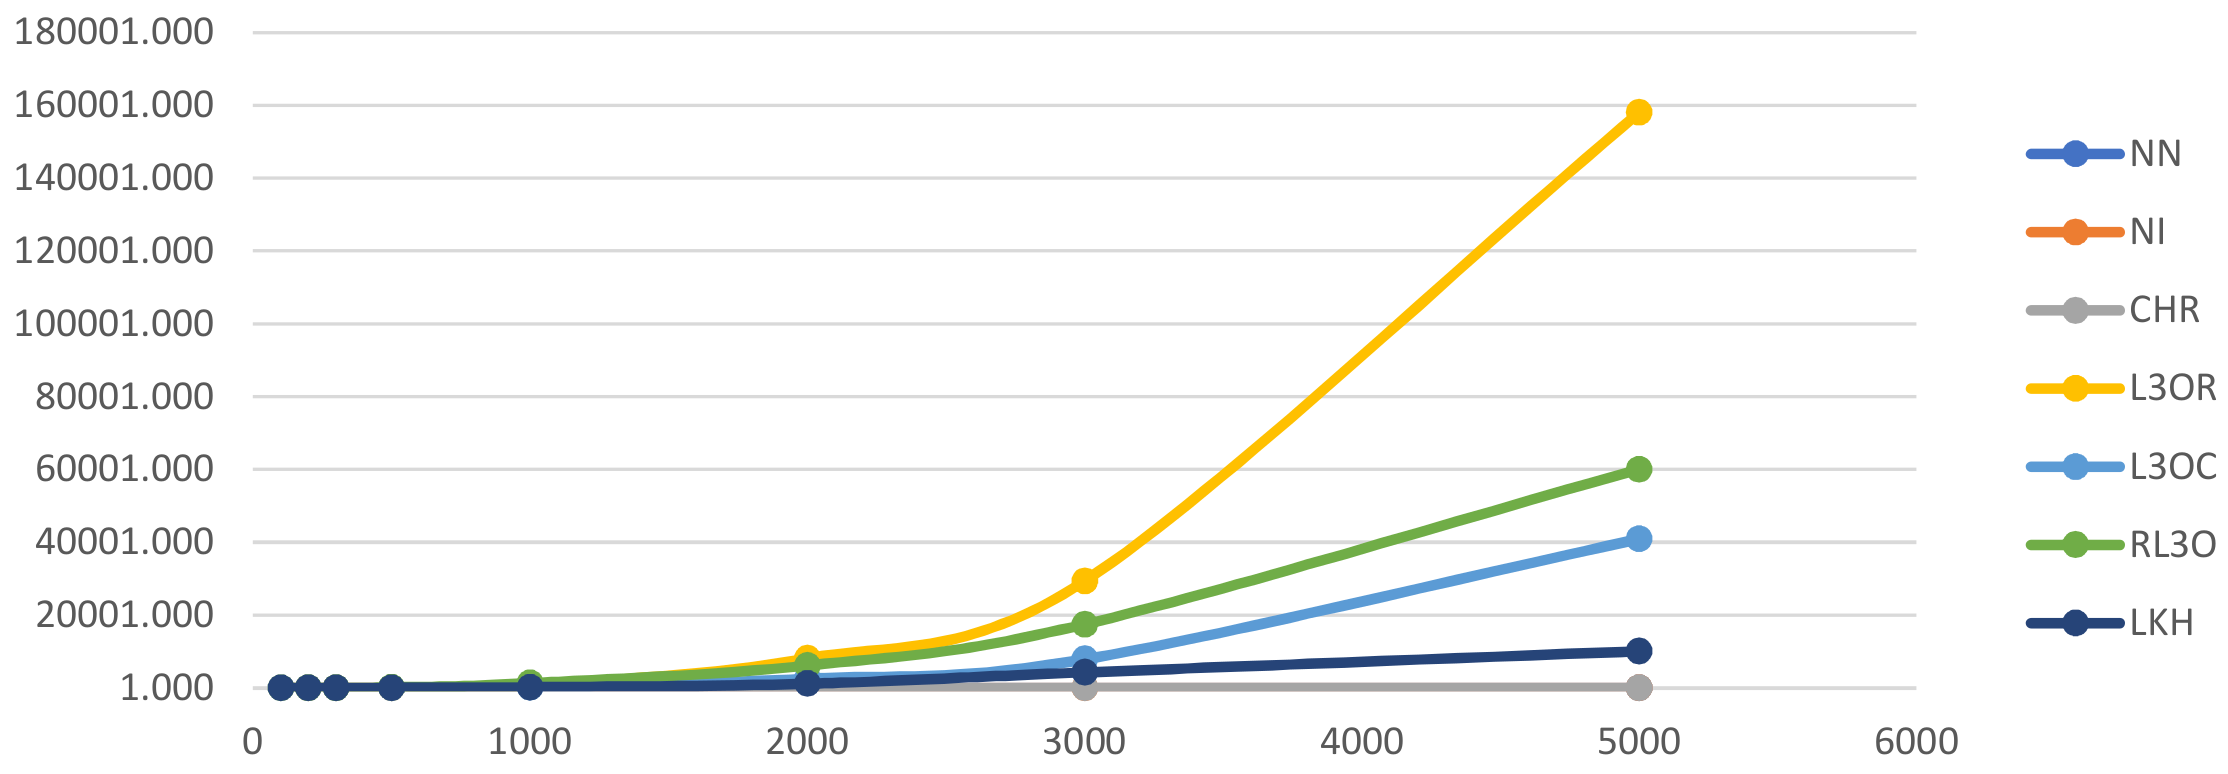
\includegraphics[width=300pt]{img/GraficoTempiRandom.png}
        \caption*{Su grafi generati casualmente.}
    \end{subfigure}
    \ \\
    \ \\
    \ \\
    \begin{subfigure}{\linewidth}
        \centering
        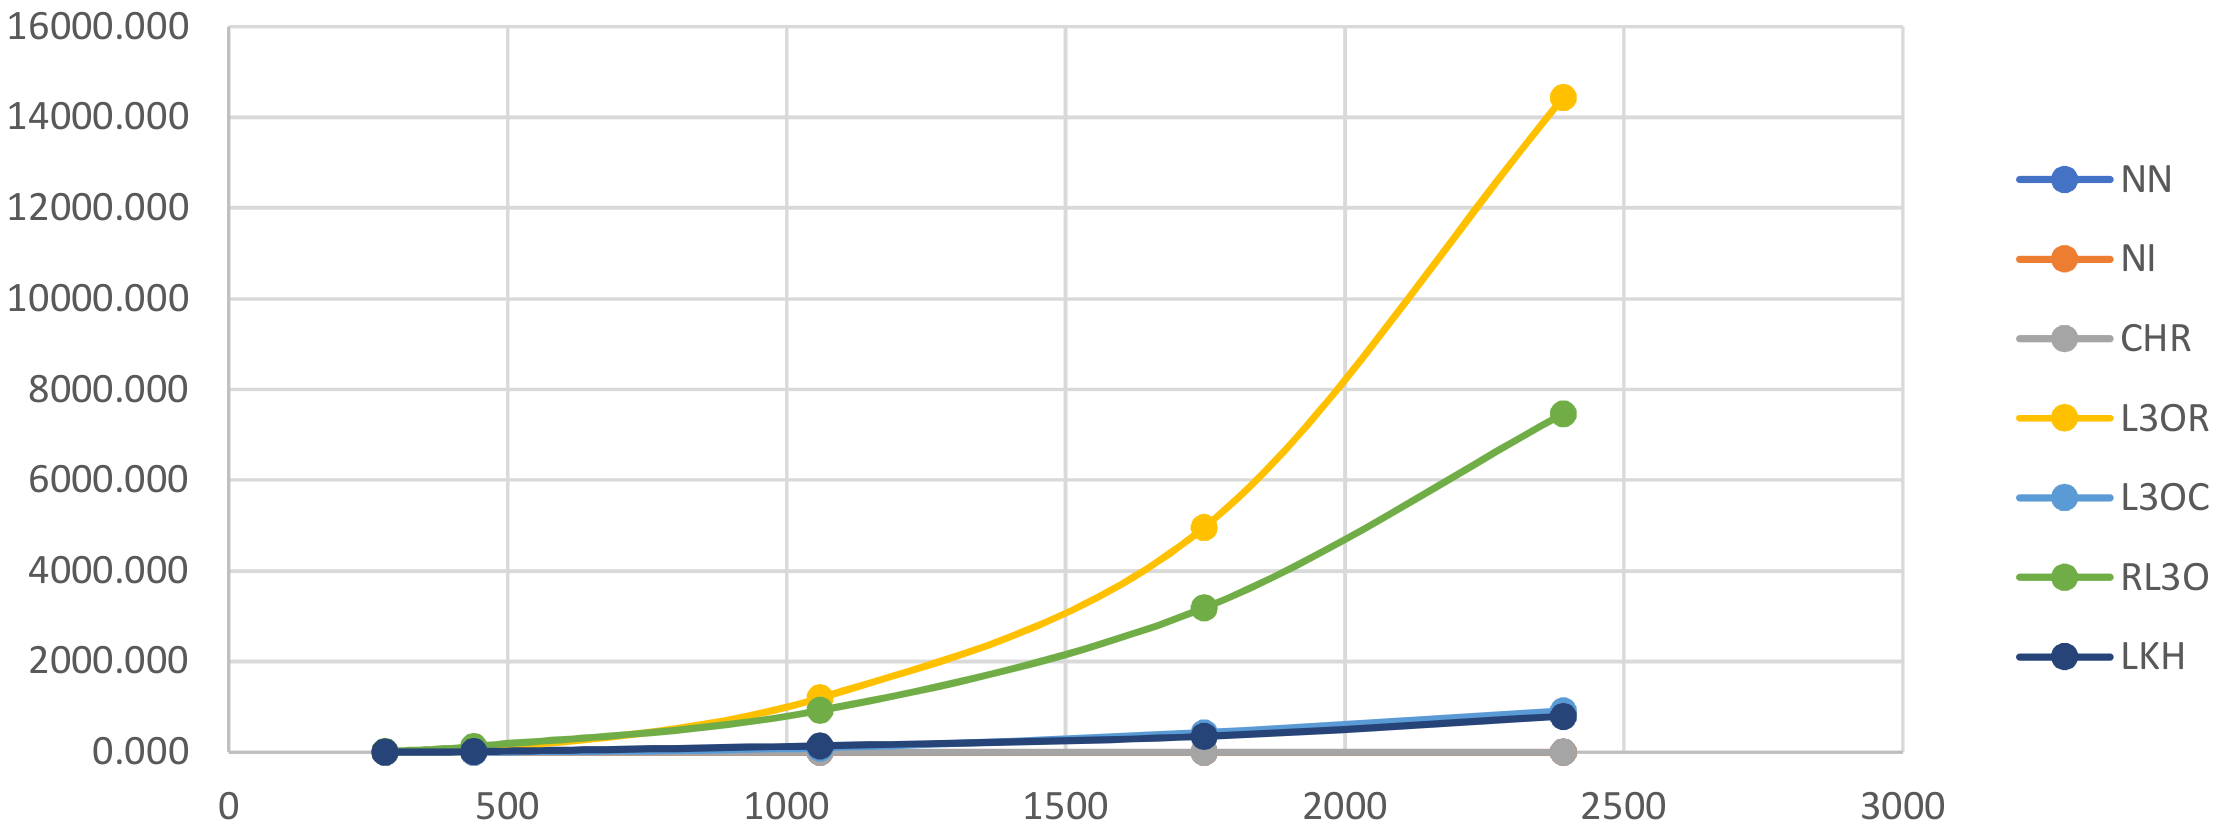
\includegraphics[width=300pt]{img/GraficoTempiTsplib.png}
        \caption*{Su grafi di \texttt{TSPLIB}.}
    \end{subfigure}
    \caption{Confronto diretto dei tempi di esecuzione delle diverse euristiche.}
\end{figure}

Da come si evince dai grafici, le euristiche ``tour construction'' sono le vincitrici per 
quanto riguarda la velocità di esecuzione; il più lento è \texttt{LR3O} con un notevole distacco (più del doppio 
del tempo rispetto al penultimo \texttt{RL3O}); \texttt{LKH} si dimostra sorprendemente veloce. Il trend si 
mantiene sia sui grafi casuali, sia sui grafi di \texttt{TSPLIB}.

\begin{figure}[H]
    \centering
    \begin{subfigure}{\linewidth}
        \centering
        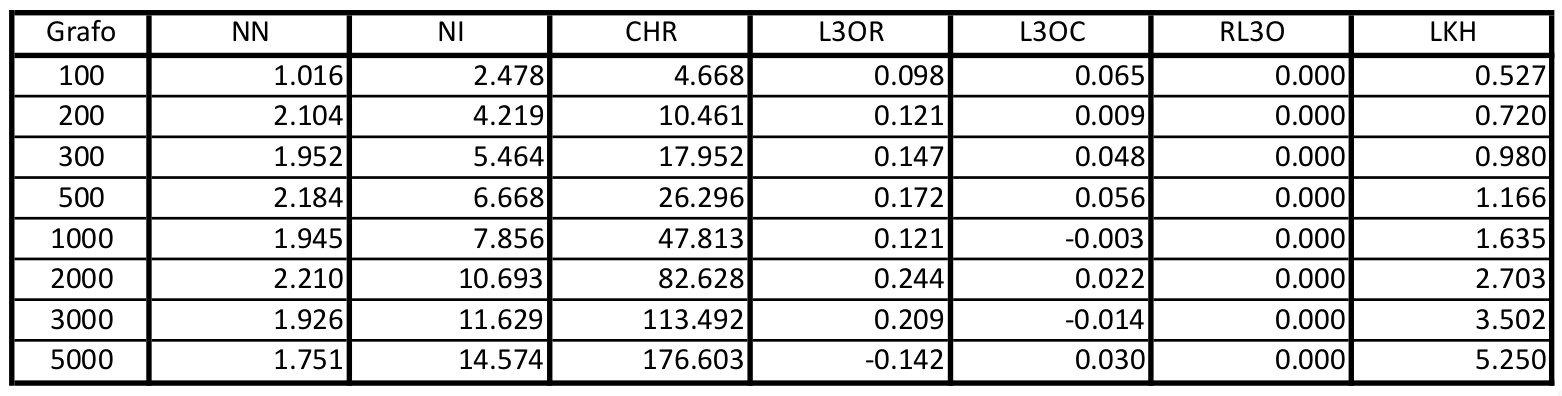
\includegraphics[width=350pt]{img/ConfrontoCostiRandom.png}
        \caption*{Su grafi generati casualmente.}
    \end{subfigure}
    \ \\
    \ \\
    \ \\
    \begin{subfigure}{\linewidth}
        \centering
        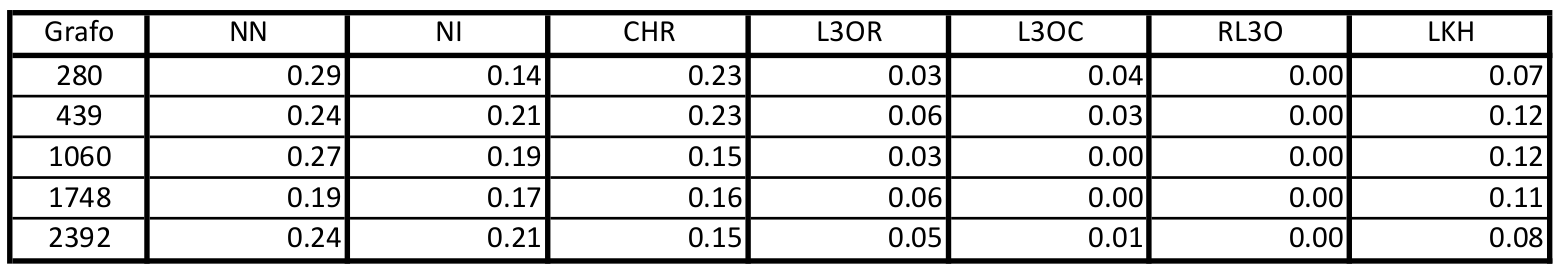
\includegraphics[width=350pt]{img/ConfrontoCostiTsplib.png}
        \caption*{Su grafi di \texttt{TSPLIB}.}
    \end{subfigure}
    \ \\
    \ \\
    \ \\
    \begin{subfigure}{\linewidth}
        \centering
        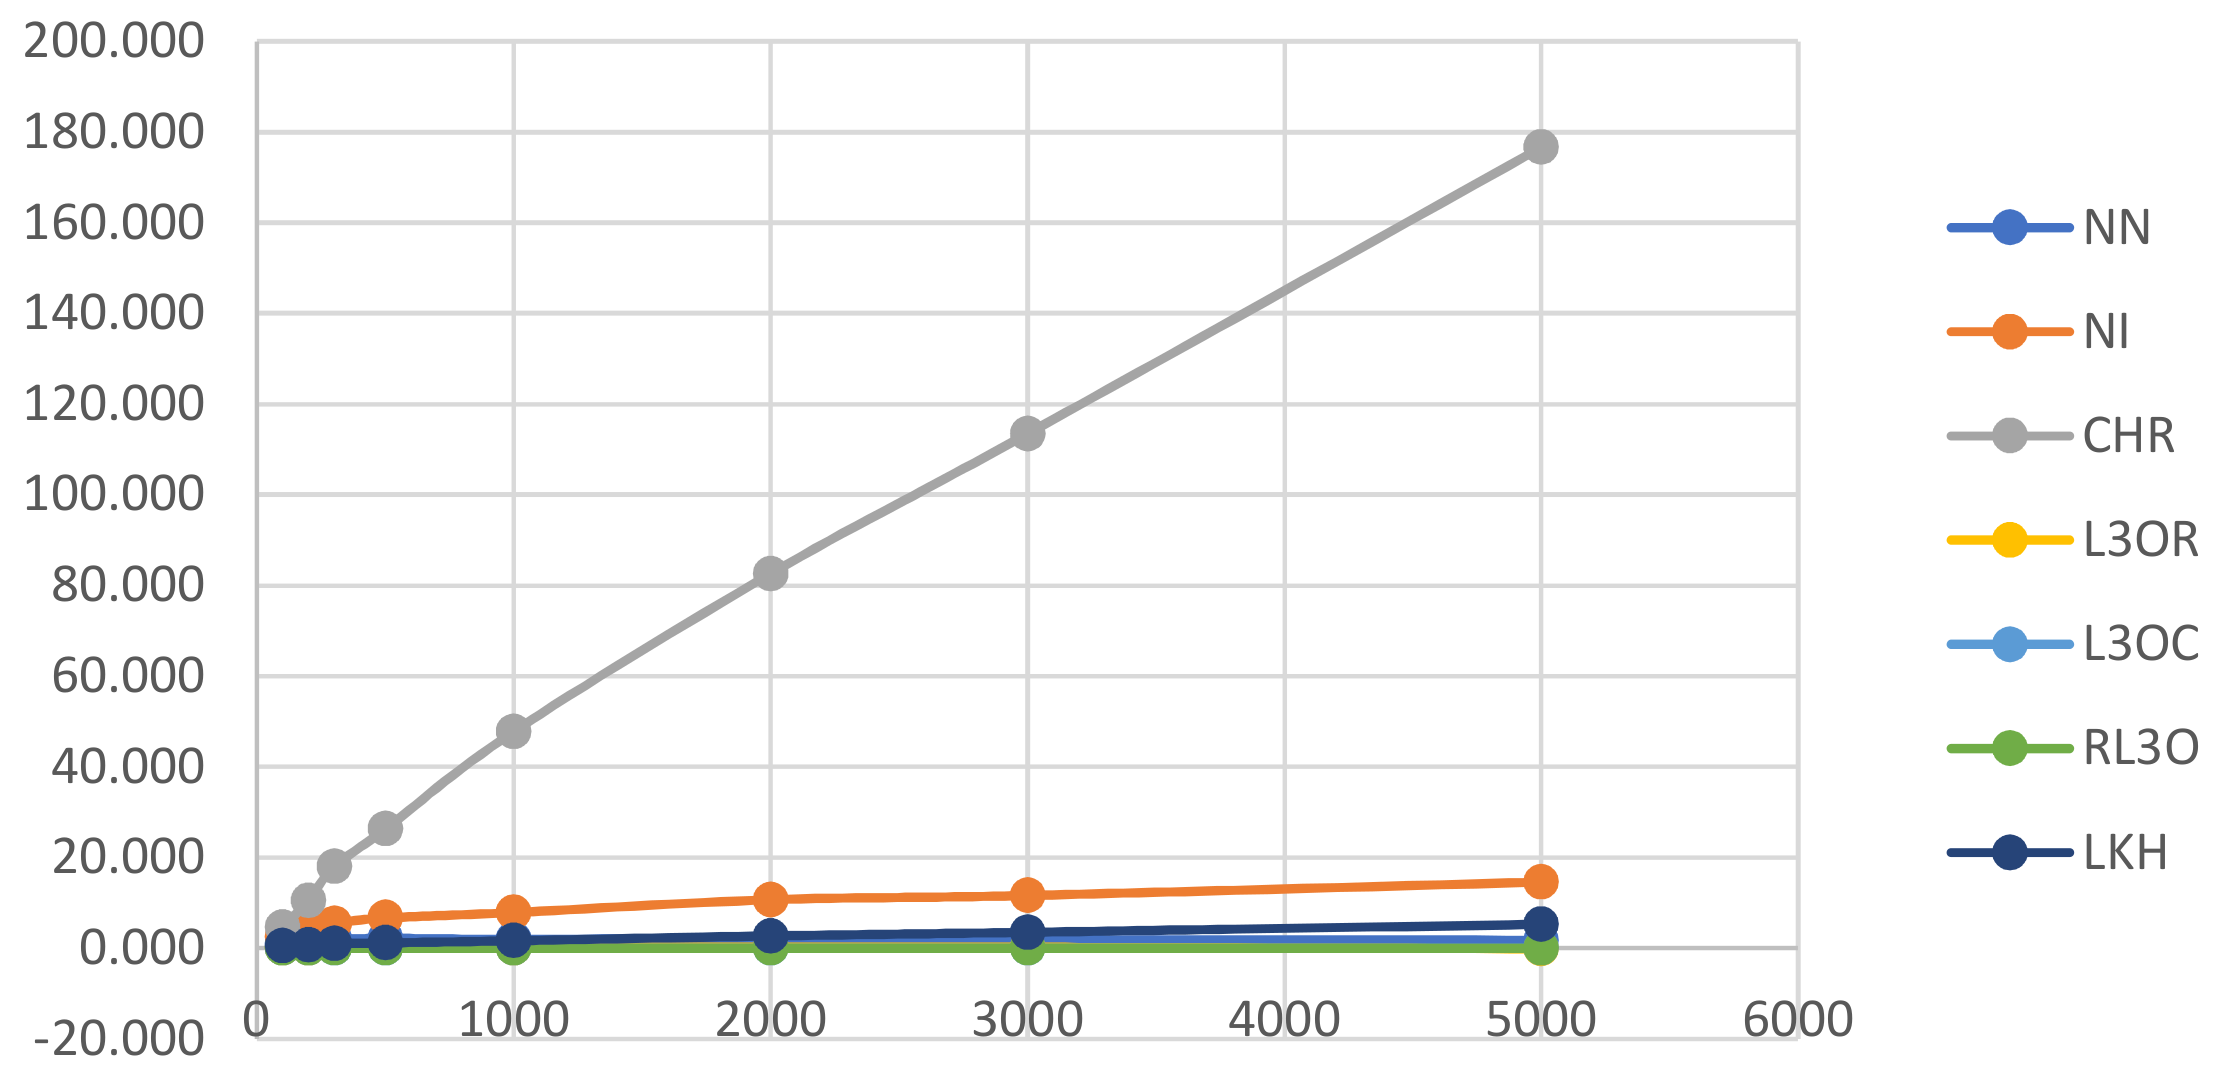
\includegraphics[width=270pt]{img/GraficoCostiRandomConCHR.png}
        \caption*{Su grafi generati casualmente, con la presenza di \texttt{CHR}.}
    \end{subfigure}
    \ \\
    \ \\
    \ \\
    \begin{subfigure}{\linewidth}
        \centering
        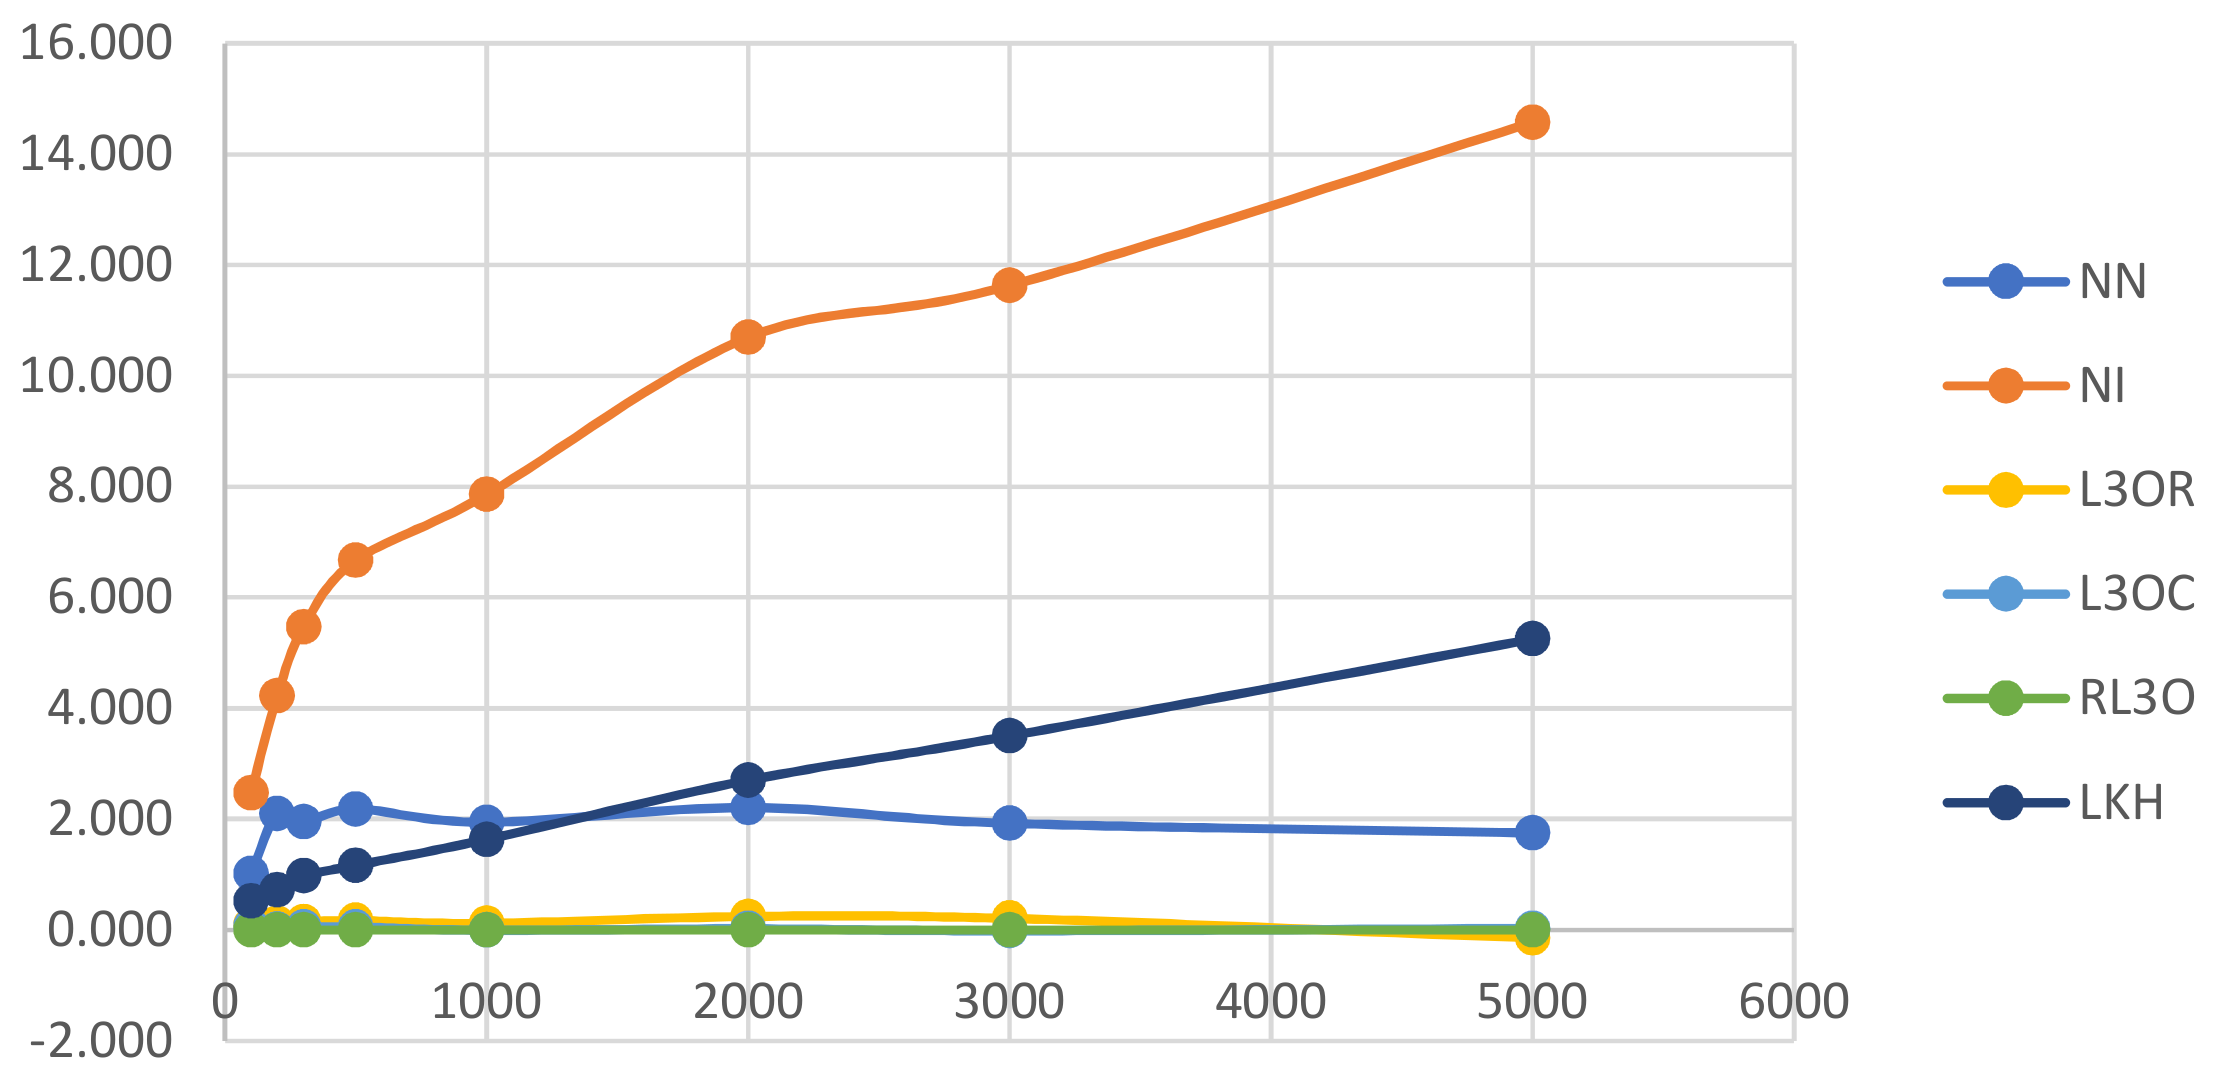
\includegraphics[width=270pt]{img/GraficoCostiRandomSenzaCHR.png}
        \caption*{Su grafi generati casualmente, senza \texttt{CHR} (che ha trovato tour 
                    molto più costosi).}
    \end{subfigure}
    \ \\
    \ \\
    \ \\
    \begin{subfigure}{\linewidth}
        \centering
        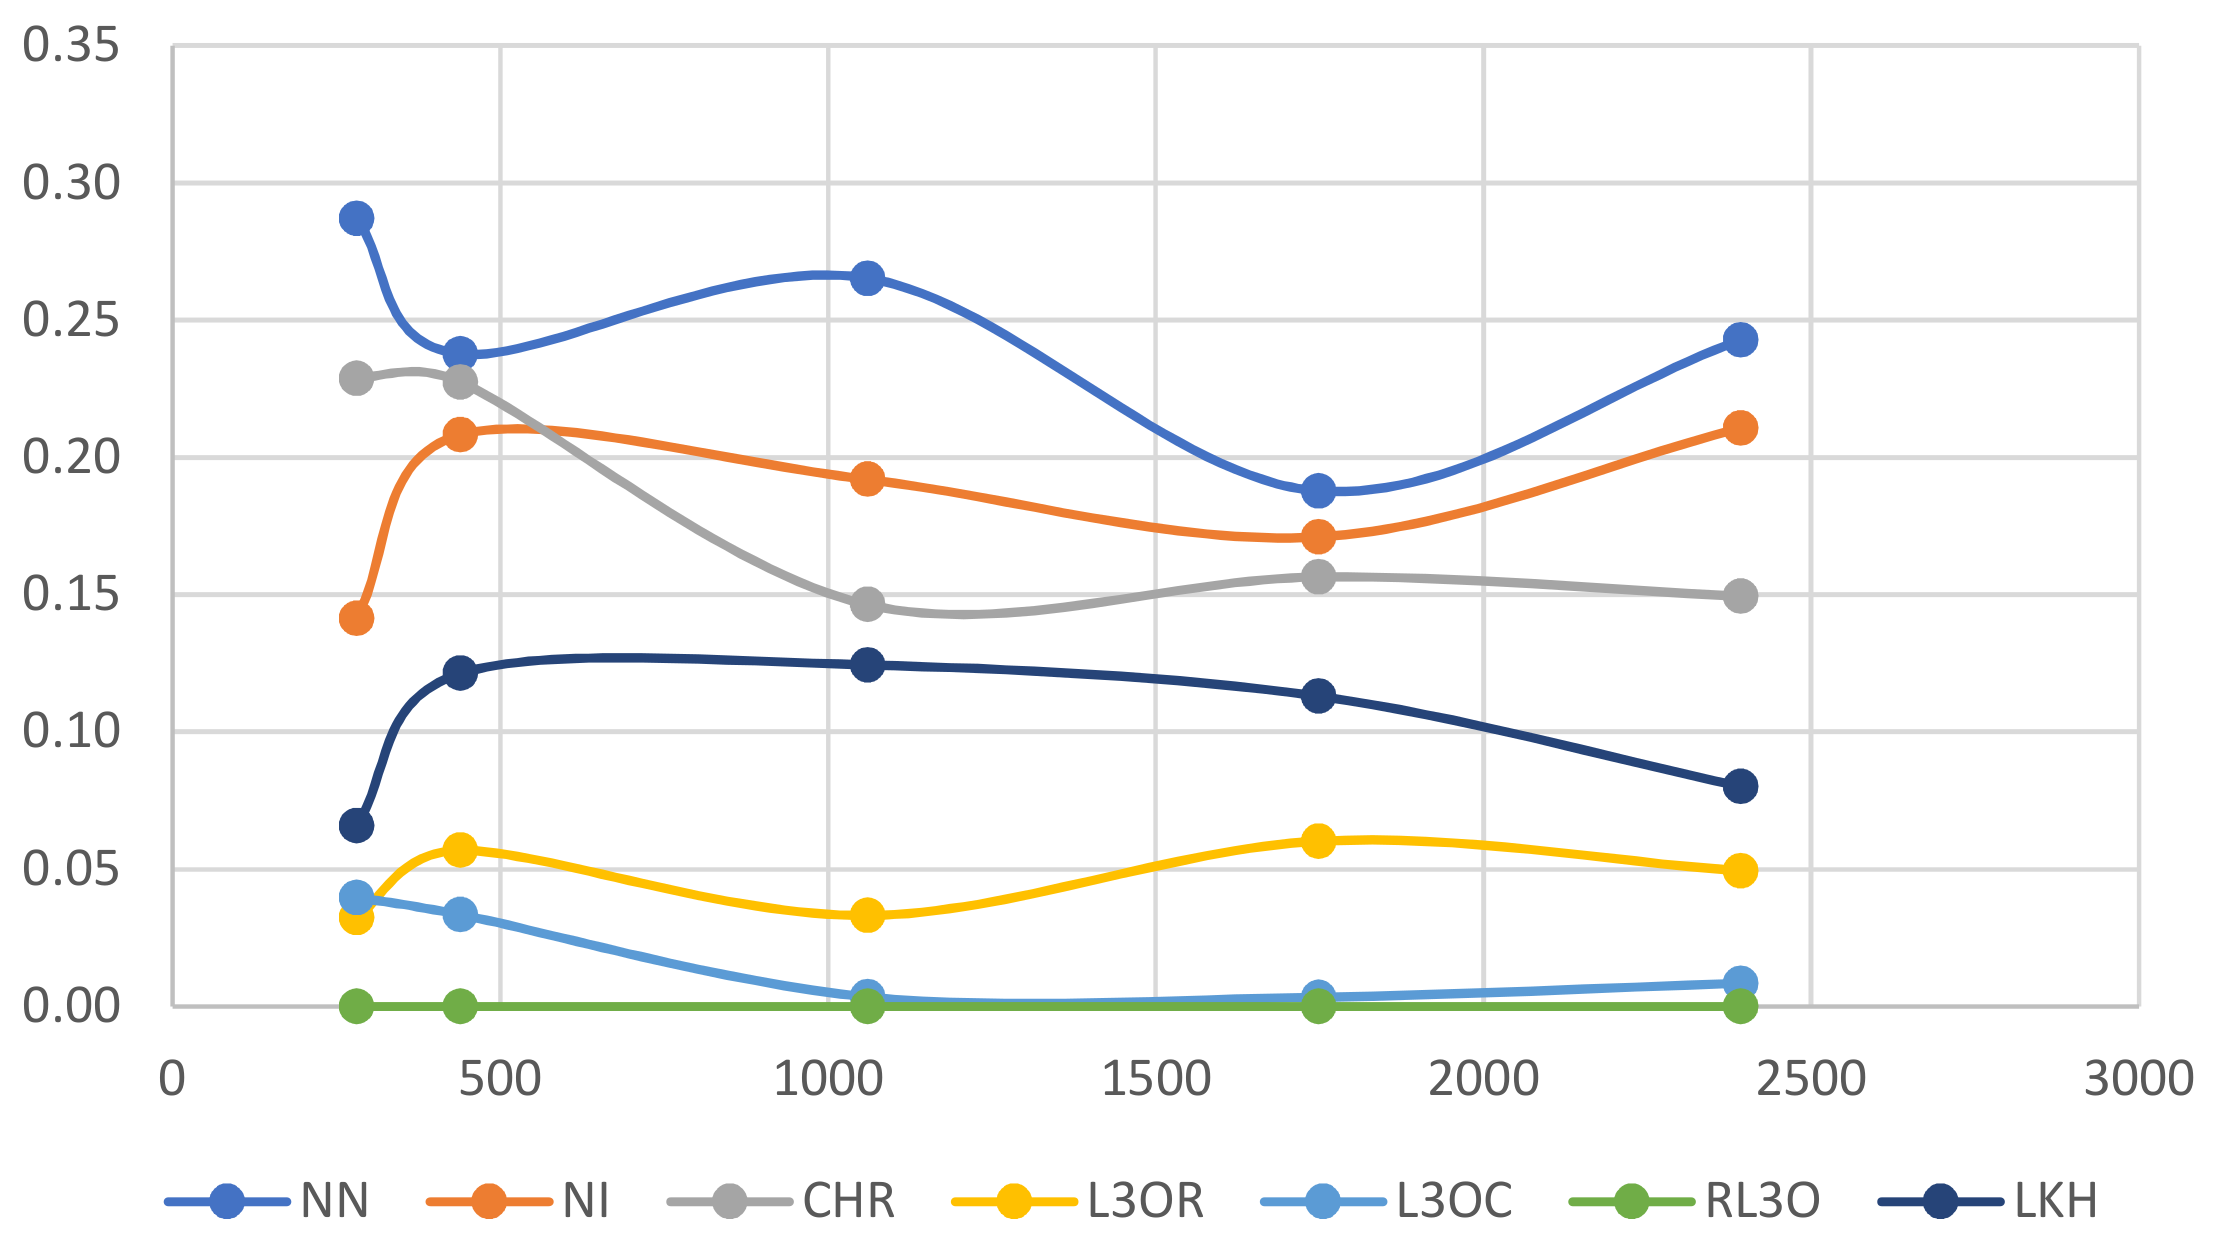
\includegraphics[width=270pt]{img/GraficoCostiTsplib.png}
        \caption*{Su grafi di \texttt{TSPLIB}.}
    \end{subfigure}
    \caption{Confronto diretto dei costi dei tour trovati dalle diverse euristiche.}
\end{figure}

Situazione diametralmente opposta per quanto riguarda i costi: \texttt{L3OR} e \texttt{RL3O} 
si dimostrano i più precisi; \texttt{CHR} decisamente impreciso per quanto riguarda i grafi 
casuali, tanto da rendere necessaria la visualizzazione grafica dei dati senza la sua presenza.
Per quanto riguarda i grafi di \texttt{TSPLIB} la situazione è più equilibrata. I confronti sui 
costi, non essendo noti gli ottimi di una delle classi di grafi, sono stati fatti in differenza 
percentuale rispetto a \texttt{RL3O}.
\ \\
\ \\

\begin{figure}[H]
    \centering
    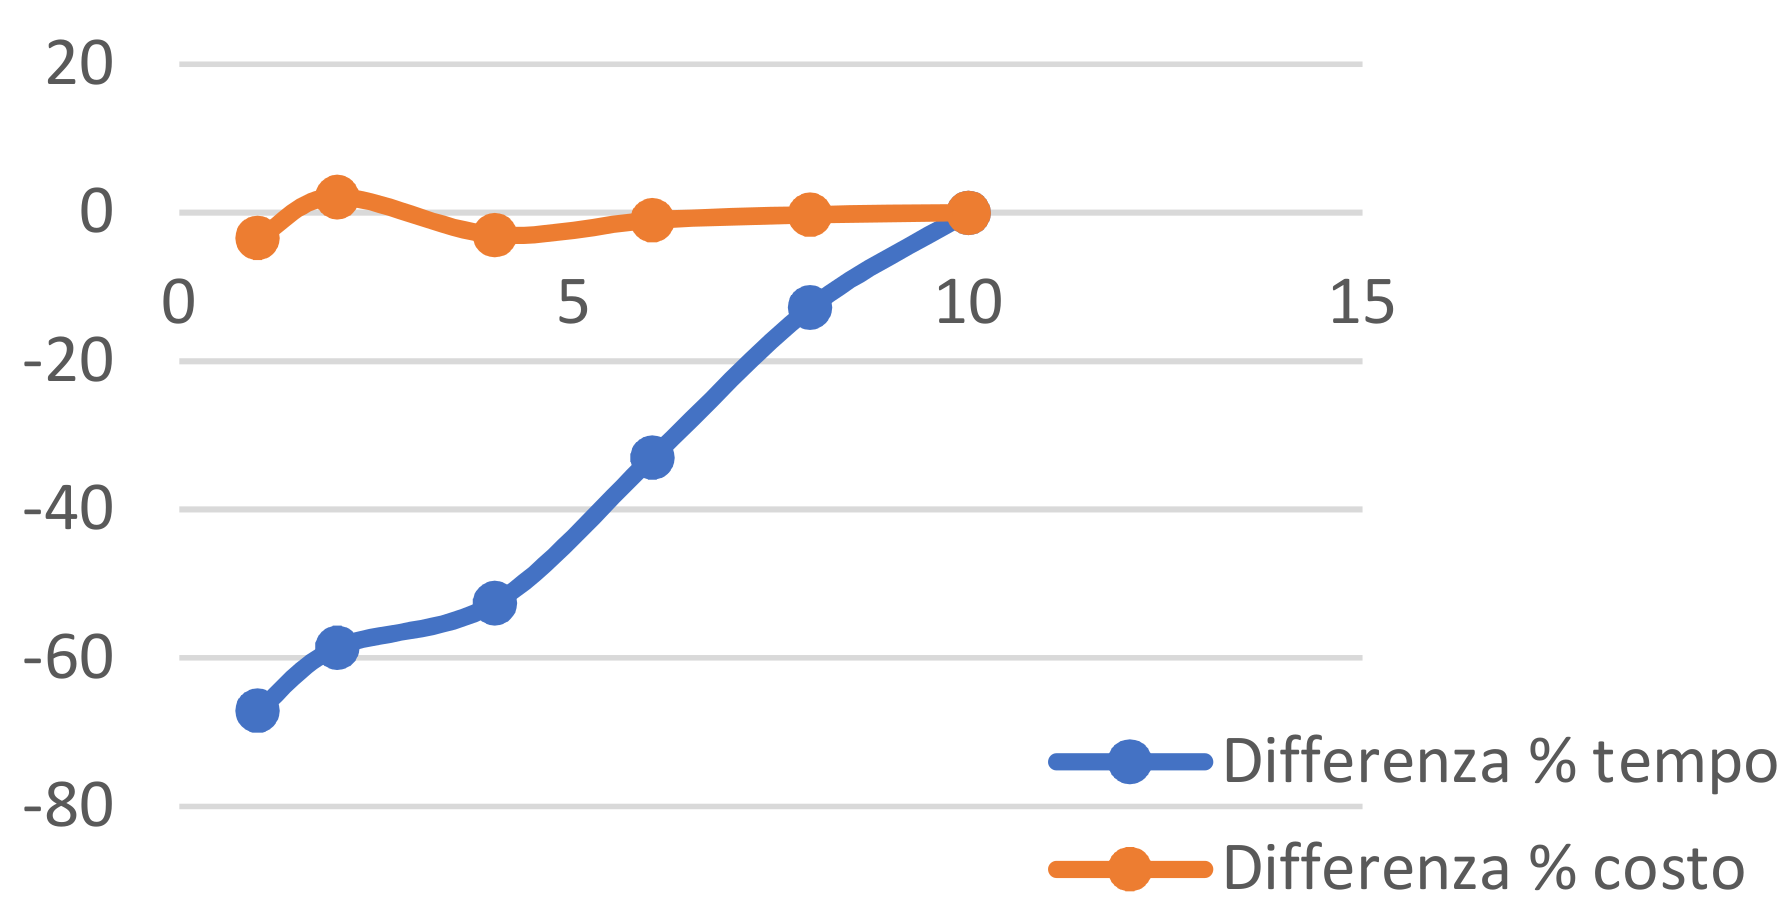
\includegraphics[width=250pt]{img/GraficoScambi.png}
    \caption{Confronto tra efficienza ed efficacia di \texttt{RL3O} al variare del numero massimo 
                di \textit{exchanges}.}
\end{figure}

Per quanto riguarda la scelta del numero massimo di scambi sembra non esserci una differenza 
sostanziale nei costi dei tour trovati quando tali scambi sono contenuti. Prevedibile, invece, 
il guadagno in tempo se riduciamo il numero di scambi: meno scambi significa, intuitivamente, che 
il tour è molto simile a prima e quindi richiede meno passi \textit{best-improving} per riottenere 
il minimo locale.
\ \\
\ \\

\begin{figure}[H]
    \centering
    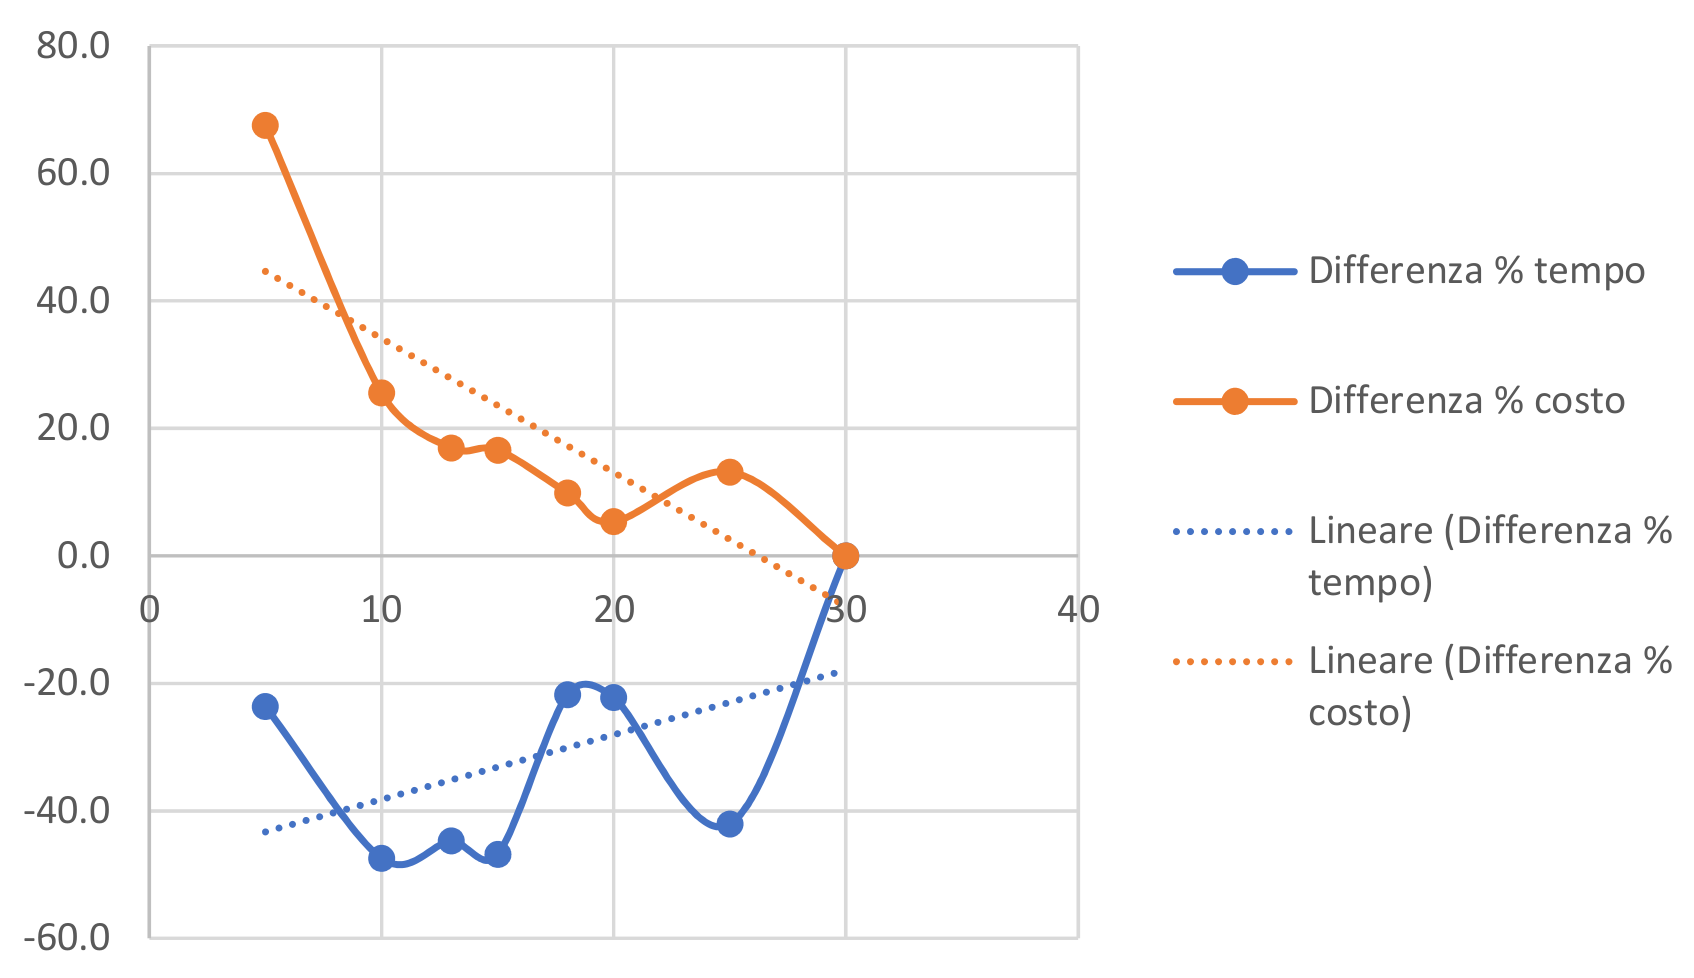
\includegraphics[width=300pt]{img/GraficoCandidati.png}
    \caption{Confronto tra efficienza ed efficacia di \texttt{LKH} al variare del numero massimo 
                di candidati per ogni \textit{candidate set}.}
\end{figure}

Prevedibile anche il risultato del test sul numero di candidati: la tendenza è quella di trovare 
tour più costosi e in meno tempo se i candidati sono pochi e tour meno costosi ma in più tempo 
se i candidati sono di più. Questo è anche il comportamento che ci si aspetterebbe da 
un'euristica, ovvero il tradeoff qualità/tempo.

% Conclusioni
\chapter{Conclusioni}

È stato presentato il Commesso Viaggiatore Simmetrico come uno dei problemi fondamentali 
dell'Ottimizzazione Combinatoria. La \textit{difficoltà} che richiede la ricerca della soluzione 
ottima e l'importanza che tale soluzione ha in svariati ambiti applicativi ci ha spinto 
a trattare il problema dal punto di vista degli algoritmi approssimati. Abbiamo presentato alcune 
delle più famose euristiche di tipo ``tour construction'', ``tour improvement'' e ``composite''. 
La famiglia ``costruttiva'' si compone di algoritmi che definiscono un tour valido vertice dopo vertice. 
La famiglia ``migliorativa'' comprende euristiche che analizzano un tour valido e cercano di modificarlo 
per ottenere un tour valido migliore. L'ultima classe si compone di algoritmi che tentano di combinare i 
vantaggi di entrambe. Abbiamo poi implementato gli algoritmi descritti e trattato, dal punto di vista empirico, 
le caratteristiche che riteniamo fondamentali in un algoritmo approssimato: velocità di esecuzione e 
errore rispetto all'ottimo; dai risultati sperimentali è emersa una correlazione tra queste due 
proprietà. Come ci si aspettava, euristiche meno elaborate impiegano meno tempo per trovare il tour 
``quasi''-ottimo, al costo di avere un elevato errore; viceversa, euristiche più elaborate impiegano 
un tempo notevolmente maggiore per trovare una soluzione, che sarà di qualità migliore. La scelta 
dell'euristica da utilizzare, tuttavia, dipende strettamente da quale caratteristica si voglia 
prediligere.

%% Parte conclusiva del documento; tipicamente per riassunto, bibliografia e/o indice analitico.
\backmatter

%% Bibliografia (opzionale)
\bibliographystyle{plain_\languagename}%% Carica l'omonimo file .bst, dove \languagename � la lingua attiva.
%% Nel caso in cui si usi un file .bib (consigliato)
\bibliography{thud}
%% Nel caso di bibliografia manuale, usare l'environment thebibliography.

%% Per l'indice analitico, usare il pacchetto makeidx (o analogo).

\end{document}

--- Istruzioni per l'aggiunta di nuove lingue ---
Per ogni nuova lingua utilizzata aggiungere nel preambolo il seguente spezzone:
    \addto\captionsitalian{%
        \def\abstractname{Sommario}%
        \def\acknowledgementsname{Ringraziamenti}%
        \def\authorcontactsname{Contatti dell'autore}%
        \def\candidatename{Candidato}%
        \def\chairname{Direttore}%
        \def\conclusionsname{Conclusioni}%
        \def\cosupervisorname{Co-relatore}%
        \def\cosupervisorsname{Co-relatori}%
        \def\cyclename{Ciclo}%
        \def\datename{Anno accademico}%
        \def\indexname{Indice analitico}%
        \def\institutecontactsname{Contatti dell'Istituto}%
        \def\introductionname{Introduzione}%
        \def\prefacename{Prefazione}%
        \def\reviewername{Controrelatore}%
        \def\reviewersname{Controrelatori}%
        %% Anno accademico
        \def\shortdatename{A.A.}%
        \def\summaryname{Riassunto}%
        \def\supervisorname{Relatore}%
        \def\supervisorsname{Relatori}%
        \def\thesisname{Tesi di \expandafter\ifcase\csname thud@target\endcsname Laurea\or Laurea Magistrale\or Dottorato\fi}%
        \def\tutorname{Tutor aziendale%
        \def\tutorsname{Tutor aziendali}%
    }
sostituendo a "italian" (nella 1a riga) il nome della lingua e traducendo le varie voci.
